\documentclass[11pt]{book}

%%%%%%%%%%%%%%Include Packages%%%%%%%%%%%%%%%%%%%%%%%%%%
\usepackage{xcolor}
\usepackage{mathtools}
\usepackage[a4paper, total={6in, 8in}, margin=1.25in]{geometry}
\usepackage{amsmath}
\usepackage{amssymb}
\usepackage{paralist}
\usepackage{rsfso}
\usepackage{amsthm}
\usepackage{wasysym}
\usepackage[inline]{enumitem}   
\usepackage{hyperref}
\usepackage{tocloft}
\usepackage{wrapfig}
\usepackage{titlesec}
\usepackage{colortbl}
\usepackage{stackengine} 
%%%%%%%%%%%%%%%%%%%%%%%%%%%%%%%%%%%%%%%%%%%%%%%%%%%%%%%%


%%%%%%%%%%%%%%%Chapter Setting%%%%%%%%%%%%%%%%%%%%%%%%%%
\definecolor{gray75}{gray}{0.75}
\newcommand{\hsp}{\hspace{20pt}}
\titleformat{\chapter}[hang]{\Huge\bfseries}{\thechapter\hsp\textcolor{gray75}{$\mid$}\hsp}{0pt}{\Huge\bfseries}
%%%%%%%%%%%%%%%%%%%%%%%%%%%%%%%%%%%%%%%%%%%%%%%%%%%%%%%%

%%%%%%%%%%%%%%%%%Theorem environments%%%%%%%%%%%%%%%%%%%
\newtheoremstyle{break}
  {\topsep}{\topsep}%
  {\itshape}{}%
  {\bfseries}{}%
  {\newline}{}%
\theoremstyle{break}
\theoremstyle{break}
\newtheorem{axiom}{Axiom}
\newtheorem{thm}{Theorem}[section]
\renewcommand{\thethm}{\arabic{section}.\arabic{thm}}
\newtheorem{lem}{Lemma}[thm]
\newtheorem{prop}[lem]{Proposition}
\newtheorem{corL}{Corollary}[lem]
\newtheorem{corT}[lem]{Corollary}
\newtheorem{defn}{Definition}[corL]
\newenvironment{indEnv}[1][Proof]
  {\proof[#1]\leftskip=1cm\rightskip=1cm}
  {\endproof}
%%%%%%%%%%%%%%%%%%%%%%%%%%%%%%%%%%%%%%%%%%%%%%%%%%%%%%


%%%%%%%%%%%%%%%%%%%%%%%Integral%%%%%%%%%%%%%%%%%%%%%%%
\def\upint{\mathchoice%
    {\mkern13mu\overline{\vphantom{\intop}\mkern7mu}\mkern-20mu}%
    {\mkern7mu\overline{\vphantom{\intop}\mkern7mu}\mkern-14mu}%
    {\mkern7mu\overline{\vphantom{\intop}\mkern7mu}\mkern-14mu}%
    {\mkern7mu\overline{\vphantom{\intop}\mkern7mu}\mkern-14mu}%
  \int}
\def\lowint{\mkern3mu\underline{\vphantom{\intop}\mkern7mu}\mkern-10mu\int}
%%%%%%%%%%%%%%%%%%%%%%%%%%%%%%%%%%%%%%%%%%%%%%%%%%%%%%



\newcommand{\R}{\mathbb{R}}
\newcommand{\N}{\mathbb{N}}
\newcommand{\Z}{\mathbb{Z}}
\newcommand{\Q}{\mathbb{Q}}
\newcommand{\C}{\mathbb{C}}
\newcommand{\T}{\mathcal{T}}
\newcommand{\M}{\mathcal{M}}
\newcommand{\Symm}{\text{Symm}}
\newcommand{\Alt}{\text{Alt}}
\newcommand{\Int}{\text{Int}}
\newcommand{\Bd}{\text{Bd}}
\newcommand{\Power}{\mathcal{P}}
\newcommand{\ee}[1]{\cdot 10^{#1}}
\newcommand{\spa}{\text{span}}
\newcommand{\sgn}{\text{sgn}}
\newcommand{\degr}{\text{deg}}
\newcommand{\pd}{\partial}
\newcommand{\that}[1]{\widetilde{#1}}
\newcommand{\lr}[1]{\left(#1\right)}
\newcommand{\vmat}[1]{\begin{vmatrix} #1 \end{vmatrix}}
\newcommand{\bmat}[1]{\begin{bmatrix} #1 \end{bmatrix}}
\newcommand{\pmat}[1]{\begin{pmatrix} #1 \end{pmatrix}}
\newcommand{\rref}{\xrightarrow{\text{row\ reduce}}}
\newcommand{\txtarrow}[1]{\xrightarrow{\text{#1}}}
\newcommand\oast{\stackMath\mathbin{\stackinset{c}{0ex}{c}{0ex}{\ast}{\Circle}}}


\newcommand{\note}{\color{red}Note: \color{black}}
\newcommand{\remark}{\color{blue}Remark: \color{black}}
\newcommand{\example}{\color{green}Example: \color{black}}
\newcommand{\exercise}{\color{green}Exercise: \color{black}}

%%%%%%%%%%%%%%%%%%%%%%Roman Number%%%%%%%%%%%%%%%%%%%%%%%
\makeatletter
\newcommand*{\rom}[1]{\expandafter\@slowromancap\romannumeral #1@}
\makeatother
%%%%%%%%%%%%%%%%%%%%%%%%%%%%%%%%%%%%%%%%%%%%%%%%%%%%%%%%%

%%%%%%%%%%%%table of contents%%%%%%%%%%%%%%%%%%%%%%%%%%%%
\setlength{\cftchapindent}{0em}
\cftsetindents{section}{2em}{3em}

\renewcommand\cfttoctitlefont{\hfill\huge\bfseries}
\renewcommand\cftaftertoctitle{\hfill\mbox{}}

\setcounter{tocdepth}{2}
%%%%%%%%%%%%%%%%%%%%%%%%%%%%%%%%%%%%%%%%%%%%%%%%%%%%%%%%%


%%%%%%%%%%%%%%%%%%%%%Footnotes%%%%%%%%%%%%%%%%%%%%%%%%%%%
\newcommand\blfootnote[1]{%
  \begingroup
  \renewcommand\thefootnote{}\footnote{#1}%
  \addtocounter{footnote}{-1}%
  \endgroup
}
%%%%%%%%%%%%%%%%%%%%%%%%%%%%%%%%%%%%%%%%%%%%%%%%%%%%%%%%%

%%%%%%%%%%%%%%%%%%%%%Section%%%%%%%%%%%%%%%%%%%%%%%%%%%%%
\makeatletter
\def\@seccntformat#1{%
  \expandafter\ifx\csname c@#1\endcsname\c@section\else
  \csname the#1\endcsname\quad
  \fi}
\makeatother
%%%%%%%%%%%%%%%%%%%%%%%%%%%%%%%%%%%%%%%%%%%%%%%%%%%%%%%%%

%%%%%%%%%%%%%%%%%%%%%%%%%%%%%%%%%%%Enumerate%%%%%%%%%%%%%%
\makeatletter
% This command ignores the optional argument 
% for itemize and enumerate lists
\newcommand{\inlineitem}[1][]{%
\ifnum\enit@type=\tw@
    {\descriptionlabel{#1}}
  \hspace{\labelsep}%
\else
  \ifnum\enit@type=\z@
       \refstepcounter{\@listctr}\fi
    \quad\@itemlabel\hspace{\labelsep}%
\fi}
\makeatother
\parindent=0pt
%%%%%%%%%%%%%%%%%%%%%%%%%%%%%%%%%%%%%%%%%%%%%%%%%%%%%%%%%%



\begin{document}

	\begin{titlepage}
		\begin{center}
			\vspace*{1cm}
			\Huge \color{red}
				\textbf{Class Notes}\\
			\vspace{0.5cm}			
			\Large \color{black}
				Math 590 - Topology\\
				Professor Nicholas McCleerey\\	
				University of Michigan\\
			\vspace{2cm}
			
\includegraphics[scale=1.15]{hmm.pdf}
			
			
			\vspace{4cm}
			\LARGE
				\textbf{Jinyan Miao}\\
				\large \textbf{and his friends from UMich Honors Math}\\
				\hfill\break
				\LARGE Fall 2022\\
			\vspace{1cm}

		\vspace*{\fill}
		\end{center}			
	\end{titlepage}

\newpage 
\tableofcontents
\addtocontents{toc}{~\hfill\textbf{Page}\par}

\newpage
\setcounter{page}{1}
\vspace*{\fill}


\newpage
Topology is the study of spaces up to continuous definition. Intuitively, we want too think of spaces as clay figures or shapes, then the continuous definition would be bending clay but not breaking or severely crashing it. \\

\example We want to say the followings are equivalent in topology:
\begin{enumerate}[topsep=3pt,itemsep=-1ex,partopsep=1ex,parsep=1ex]
\item A circle of radius $1$.
\item A circle of radius $2$.
\item A triangle.
\item A square.
\item A polygon
\end{enumerate}
Such example should motivate need for new invariants of a space, which are preserved under continuous definition. For example, the boundary of a space should be invariant under continuous definitions. An interval and a circle are not equivalent because turning interval into the transformation between them involves destroying end points. Another thing that is preserved under continuous definition is thee number of loops in the shape. That is, for example, a circle is not equivalent to the shape ``$\infty$'', because the former has only one enclosed area, but the later has two enclosed areas. \\

We will first define topological spaces and their equivalences defined by the homeomorphisms. Then we will study  the properties that are preserved by the homeomorphisms.\\

In this text, we denote a set as capital letters, such as $A$. Elements in set $A$ are usually denoted as $a \in A$. Cursive fonts of capital letters such as $\mathcal{A}$ will be used to denote the set of sets. Cursive fonts of some particular letters are usually used to denote the index sets, such as $\mathcal{I}, \mathcal{J}, \mathcal{K}$. For example, the union of sets, and the intersection of sets, are written as the followings:
\begin{align*}
\bigcup_{\alpha \in \mathcal{I}} A_\alpha \qquad\qquad\qquad \bigcap_{\alpha \in \mathcal{I}}A_{\alpha}
\end{align*}
The product of sets usually refers to the Cartesian Product of sets, denoted as:
\begin{align*}
\prod_{\alpha \in \mathcal{I}} A_{\alpha}
\end{align*}
The power set of $A$ is denoted as $\Power(A)$, which is the collection of subsets of $A$. \\

$\Z$ is countably infinite, and $w \coloneqq |\Z|$ is the cardinality of $\Z$. Hence we define the following to be the countable product of a set $A$:
$$A^w \coloneqq \prod_{i=1}^\infty A$$
For order relations, simple orders of a set is also called the total order of the set. We will switch from total orders to partial orders if needed. \\


\newpage
\chapter{The Topology}
\section[Basis of Topology]{\color{red}Basis of Topology\color{black}}
\begin{defn}
Let $X$ be a set, a topology $\tau$ on $X$ is a collection of subsets of $X$ satisfying all of the following conditions:
\begin{enumerate}[topsep=3pt,itemsep=-1ex,partopsep=1ex,parsep=1ex]
\item $\emptyset, X$ are elements in $\tau$
\item For $\{ U_\alpha \mid \alpha \text{ belongs to an index set}\}\subseteq \tau$, we have $\bigcup_{\alpha} U_\alpha \in \tau$
\item For $\{ U_\alpha \mid \alpha \text{ belongs to a finite index set}\}\subseteq \tau$, we have $\bigcap_{\alpha} U_\alpha \in \tau$
\end{enumerate} 
Elements in $\tau$ are called open subsets of $X$, and $(X,\tau)$ constitutes a topological space.
\end{defn}

\example Consider the set $\R$, equipped with the standard Eculidean topology $\tau_{EUC}$ constitutes a topological space. Elements in $\tau_{EUC}$ can be expressed as a union of open intervals.\\

\example Let $X$ be a set, and consider $\tau =\Power(X)$. Here $(X,\tau)$ constitutes a topological space. Here $\Power(X)$ is called the discrete topology on $X$.\\

\example Let $X$ be a set, and consider $\tau =\{X,\emptyset\}$. Here $(X,\tau)$ constitutes a topological space. Here $\{X,\emptyset\}$ is called the indiscrete topology, or the trivial topology, on $X$. This behavior leads to the separation axiom in topology.\\


\begin{defn}[First Separation Axiom]
The topological space $(X,\tau)$ is $T_1$, or it satisfies the first separation axiom, provided that any $x,y \in X$, there exists $U \in \tau$ such that $x \notin U$ but $y \in U$. 
\end{defn}


\example The discrete topology is always $T_1$, but the indiscrete topology is never $T_1$. \\

\example $\R$ equipped with the Euclidean topology is $T_1$. \\

\remark The behavior of equipping a set with discrete topology is seen as pathological.
Further separation axioms $T_2$, $T_3$, and so on, characterize spaces to be less pathological.\\

\begin{defn}
A basis for a topology is a collection $\mathcal{B}$ of subsets of $X$ such that the followings hold:
\begin{enumerate}[topsep=3pt,itemsep=-1ex,partopsep=1ex,parsep=1ex]
\item For all $x \in X$, there exists $U \in \mathcal{B}$ such that $x \in U$
\item If $x \in B_1 \cap B_2$ for some $B_1,B_2 \in \mathcal{B}$, then $\exists\ B_3 \in \mathcal{B}$ such that $x \in B_3 \subseteq B_1 \cap B_2$
\end{enumerate}
The topology generated by $\mathcal{B}$ is denoted as $\tau_\mathcal{B}$, defined by the following:
\begin{align*}
\tau_{\mathcal{B}} \coloneqq \left\{U = \bigcup_{\alpha\in \mathcal{J}}V_\alpha \mid \mathcal{J} \text{ is an index set, and for all }\alpha \in \mathcal{J},\ V_{\alpha} \in\mathcal{B}\right\}
\end{align*}
\end{defn}

\example $\R$ equipped with the Euclidean topology is generated by the basis consists of only open intervals, and in such case $\tau_{\mathcal{B}} = \tau_{EUC}$.\\


\example Consider a set $X$, the discrete topology of $X$ is generated by the singletons in $X$, that is, the basis of the discrete topoly on $X$ is given by the following: 
\begin{align*}
\mathcal{B} = \{ \{x\} \mid x \in X\}
\end{align*}

\begin{lem}
For a set $X$ and a topological basis $\mathcal{B}$ on $X$, $\tau_{\mathcal{B}}$ is a topology on $X$.
\end{lem}
\begin{proof}
Clearly we have $\emptyset, X \in \tau_\mathcal{B}$. Cosndier $\{U_\alpha \mid \alpha \in \mathcal{J}\}\subseteq \tau_{\mathcal{B}}$ with $\mathcal{J}$ being an arbitrary index set, by definition, we can write the following for all $\alpha \in \mathcal{J}$:
\begin{align*}
U_\alpha = \bigcup_{\beta \in I_\alpha} V_\beta
\end{align*}
where $V_{\beta} \in \mathcal{B}$ for all $\beta \in I_\alpha$ and $I_\alpha$ is an index set. Then we can write the following:
\begin{align*}
\bigcup_{\alpha \in \mathcal{J}}U_\alpha = \bigcup_{\alpha \in \mathcal{J}}\bigcup_{\beta \in I_{\alpha}}V_\alpha \in \tau_{\mathcal{B}}
\end{align*}
Now consider $U_1,U_2,\cdots, U_m \in \tau_\mathcal{B}$, we can proceed using induction to show that intersection of $U_n$ for all $1\leq n \leq m$ belongs to $\tau_{\mathcal{B}}$. Here it suffices to check the base case, where we can write:
\begin{align*}
U_1 \cap U_2 = \left( \bigcap_{\alpha \in I_1}V_\alpha\right) \cap \left( \bigcup_{\beta \in I_2}V_\beta\right)
\end{align*}
with $I_1,I_2$ being index set, and $V_\alpha,V_\beta \in \mathcal{B}$ for all $\alpha \in I_1$ and $\beta \in I_2$. If $x \in U_1 \cap U_2$, then there exists $\alpha \in I_1$ and $\beta \in I_2$ such that $x \in V_\alpha \cap V_\beta$, then hence there exists $V_{\alpha\beta} \in \mathcal{B}$ such that $x \in V_{\alpha\beta}\subseteq V_\alpha \cap V_{\beta} \subseteq U_1 \cap U_2$, that is $U_1 \cap U_2 = \bigcup_{\alpha,\beta} V_{\alpha\beta}$.
\end{proof}

\begin{defn}
Let $X$ be a set, and let $\mathcal{S} \subseteq \Power(X)$. $\mathcal{S}$ is called a topological subbasis provided that the union of all elements of $\mathcal{S}$ is $X$. The topology generated by $\mathcal{S}$ is the collection given by:
\begin{align*}
\tau_{\mathcal{S}}\coloneqq \{ \text{all unions of finite intersections of elements in }\mathcal{S}\}
\end{align*}
\end{defn}

\begin{defn}
Let $X$ be a set, let $\tau_1$ and $\tau_2$ be topologies on $X$. $\tau_1$ is said to be finer than $\tau_2$ provided that $\tau_1 \subseteq \tau_2$, in which case we say $\tau_1$ and $\tau_2$ are comparable, and $\tau_2$ is coarser than $\tau_1$. 
\end{defn}

\begin{prop}
Let $\mathcal{B}$ be a basis for a topology on a set $X$. $\tau_{\mathcal{B}}$ is the coarsest topology containing $\mathcal{B}$.
\end{prop}
\begin{proof}
If $\tau$ is a topology with $\mathcal{B} \subseteq \tau$, we want to show that $\tau_{\mathcal{B}} \subseteq \tau$. If $U \in \tau_{\mathcal{B}}$, then we know that $U = \bigcup_{\alpha \in \mathcal{J}}V_\alpha$ with $V_\alpha \in \mathcal{B}$ for all $\alpha$ in the index set $\mathcal{J}$, that is $U \in \tau$. 
\end{proof}

\begin{lem}[Lemma 13.3 on Munkres]
Let $\mathcal{B}$ and $\mathcal{B}'$ be basis for topologies $\tau$ and $\tau'$, respectively, on a set $X$. Then $\tau'$ is finer than $\tau$ if and only if for all $x \in X$ such that $x \in U\in \mathcal{B}$, there exists $U' \in \mathcal{B'}$ such that $x \in U' \subseteq U$. That is $U = \bigcup_{\alpha \in \mathcal{J}}U'_{\alpha}$, for some $\{ U_\alpha' \mid \alpha \in \mathcal{J}\}\subseteq \mathcal{B}'$
\end{lem}
\begin{proof}
The $\Leftarrow$ direction is clear from the statement. For the $\Rightarrow$ direction, we suppose that $U \in \tau$, we want to show that $U \in \tau'$. Note that $\tau'$ is generated by $\mathcal{B}'$, that is, we can write:
\begin{align*}
U = \bigcup_{\alpha \in \mathcal{J}} U_\alpha
\end{align*}
for some collection $\{ U_{\alpha}\mid \alpha \in \mathcal{J}\} \subseteq \mathcal{B}'$ with $\mathcal{J}$ being an index set.
\end{proof}


\newpage
\section[Order Topology]{\color{red}Order Topology\color{black}}
\begin{defn}
A set $X$ is partially ordered with respected to the relation $\leq$ provided that we have all of the followings hold:
\begin{enumerate}[topsep=3pt,itemsep=-1ex,partopsep=1ex,parsep=1ex]
\item $a\leq a$ for all $a \in X$.
\item For $a,b \in X$, we have $a\leq b$ and $b \leq a$ if and only if $a= b$.
\item For $a,b,c \in X$, if we have $a\leq b$, and $b\leq c$, then $a\leq c$.
\end{enumerate}
A partially ordered set $X$ with respect to the relation $\leq$ is denoted as $(X,\leq)$.
\end{defn}

\example Let $X$ be any nonempty set, then the set $\Power(X)$ is a partially ordered set with respect to the relation $ \subseteq$. \\

\note For a partially ordered set $X$ with the relation $\leq$, for $a,b \in X$, we write $a<b$ if and only if $a\leq b$ and $a\neq b$.

\begin{defn}
A set $X$ is said to be totally ordered with respect to the relation $\leq$ provided that $X$ is a partially ordered set and for any $a,b \in X$, we have either $a\leq b$ or $b \leq a$. A totally ordered set $X$ with respect to the relation $\leq$ is denoted as $(X,\leq)$. \footnote{A totally ordered set is also called a simply ordered set, or a linearly ordered set}
\end{defn}


\begin{defn}
Let $(X,\leq)$ be a totally ordered set, in the case where $X$ is not bounded above or below, the order topology on $(X,\leq)$ is the topology generated by the following basis:
\begin{align*}
\mathcal{B} \coloneqq \{ (a,b) \mid a,b \in X,\ a<b\}\qquad\qquad (a,b) \coloneqq \{ x \in X \mid a<x<b\}
\end{align*}
If there exists some maximal element $a_0\in X$, and, or, some minimal element $b_0 \in X$, the order topology on $(X,\leq)$ is the topology generated by the following basis:
\begin{align*}
\mathcal{B} \coloneqq \{ (a,b),\ [a_0,b),\  (a,b_0] \mid a,b \in X,\ a<b\}
\end{align*}
\end{defn}

\example The Euclidean topology on $\R$ is the ordered topology on $\R$.\\

\begin{defn}
Let $(X,\leq_X)$ and $(Y, \leq_Y)$ be totally ordered sets, a total order on $X\times Y$, called the dictionary order, is defined by the condition that, for $x_1,x_2 \in X$ and $y_1,y_2 \in Y$, we say $x_1 \times y_1 \leq x_2 \times y_2$ provided that we have either $x_1 <_X x_2$, or $x_1 = x_2$ with $y_1 \leq_Y y_2$. 
\end{defn}

\example Let $\R^2 \coloneqq \R \times \R$ be equipped with the dictionary ordering coming from the usual ordering on $\R$. For $a,b,c,d \in \R$, we can write:
\begin{align*}
\left( a\times b, c\times d\right) \coloneqq \{ x \times y \in \R^2 \mid a\times b < x\times y < c\times d \}
\end{align*}
Here we get the following cases:
\begin{enumerate}
\item If we have $a<c$, then all vertical lines with $x$-component strictly greater than $a$ and strictly less than $c$ on the $\R^2$-plane are included in $\left( a\times b, c\times d\right)$, and $\left( a\times b, c\times d\right)$ also includes the vertical ray with components $x =a$, $y>b$, and the vertical ray with components $x=c$, $y<d$. That is, we write:
\begin{align*}
\left( a\times b, c\times d\right) = \{ x\times y \in \R^2 \mid a<x<c \text{, or }a=x \text{ with } y>b \text{, or }c=x \text{ with } y<d\}
\end{align*} 
\item In the case $a=c$, we have:
\begin{align*}
\left( a\times b, c\times d\right) = \{ a\times y \in \R^2 \mid b<y<d\}
\end{align*}
In such case $\left( a\times b, c\times d\right)$ is a line segment and it behaves as an open interval in $\R^2$ when equipped with the dictionary order and order topology.
\end{enumerate}

\remark Intuitively, $\R$ is a $1$-dimensional space, so we would like to have $\R^2$ being $2$-dimensional space. However, $\R^2$ equipped with the dictionary topology looks like a bunch of $1$-dimensional spaces stacked on top on one another, as seen in the second case of the example above.

\newpage
\section[Product Topology]{\color{red} Product Topology\color{black}}
\begin{defn}
Let $(X,\tau_X)$ and $(Y,\tau_Y)$ be topological spaces, we define:
\begin{align*}
\mathcal{B} \coloneqq \{ U \times V \mid U \in \tau_X \text{ and } V \in \tau_Y\}
\end{align*}
Here $\mathcal{B}$ defines a basis for a topology on $X \times Y$ called the product topology.
\end{defn}

\example The Euclidean topology on $\R^2$ is the product topology on $\R \times \R$. Note that, when equipped with the Euclidean topology, the union of two open rectangles in the $\R^2$ plane is also open, no matter whether the rectangles overlap or not, but in the case where the two rectangles overlap, their union does not belong to $\mathcal{B}$.


\begin{prop}
Let $\mathcal{B}_X$ and $\mathcal{B}_Y$ be topological bases for $(X,\tau_X)$ and $(Y,\tau_Y)$, respectively, then the following defines a topological basis for the product topology on $X \times Y$: \footnote{Thereafter, the product of sets $X \times Y$ without an explicit topology being specified is assumed to be equipped with the product topology.}
\begin{align*}
\that{\mathcal{B}}\coloneqq \{ U \times V \mid U \in \mathcal{B}_X \text{ and }V \in \mathcal{B}_Y\}
\end{align*}
\end{prop}
\begin{proof}
Given $U \times V \in \{ U \times V \mid U\in \tau_X \text{ and }V \in \tau_Y\}$, we see that $U$ is open in $X$, and $V$ is open in $Y$, hence there exist $U_\beta \in \mathcal{B}_X$ for all $\beta$ in an index set $\mathcal{L}$ such that: 
$$U = \bigcup_{\beta \in \mathcal{L}} U_\beta$$ 
and similarly, there exists $V_\gamma \in \mathcal{B}_Y$ for all $\gamma $ in an index set $\mathcal{K}$ such that $$V = \bigcup_{\gamma \in \mathcal{K}}V_\gamma$$ 
Then we can write the following:
\begin{align*}
U \times V = \bigcup_{\beta\in \mathcal{J},\ \gamma\in \mathcal{K}} U_\beta \times V_\gamma
\end{align*}
which concludes the result.
\end{proof}

\note The basis $\that{\mathcal{B}} = \{U\times V\mid U \in \mathcal{B}_X \text{ and }V\in \mathcal{B}_Y\}$ on $\R^2$ is the set of open rectangles on the $\R^2$ plane. Here $\that{\mathcal{B}}$ is equivalent to the basis of all open balls on $\R^2$, as one can view open balls as unions of open rectangles, and open rectangles as union of open balls. \\

\begin{defn}
For sets $X, Y$, consider the product $X\times Y$. The projection maps on $X\times Y$ are defined by the followings:
\begin{align*}
\Pi_X: X\times Y \to X \qquad x\times y \mapsto x\qquad\qquad\qquad\qquad \Pi_Y:X\times Y\to Y \qquad x\times y \mapsto y
\end{align*}
\end{defn}
\newpage
\begin{prop}
Let $(X,\tau_X)$ and $(Y,\tau_Y)$ be topological spaces. The following collection forms a subbasis for the product topology on $X\times Y$:
\begin{align}
\mathcal{S} = \{ \Pi_X^{-1}(U) \mid U \in \tau_X\}\cup \{ \Pi_Y^{-1}(V) \mid V \in \tau_Y\}
\end{align}
\end{prop}
\begin{proof}
First we will show that $\Pi_X^{-1}(U) = U \times Y$ for $U \in \tau_X$. Let $v \in \Pi_{X}^{-1}(U)$, then we have $\Pi_X(v)\in U$, so if $v = (x,y)$, then $\Pi_X(v) = x \in U$, that is $v \in U \times Y$. On the other hand, for $(x,y) \in U \times Y$, then by definition, $x \in U$ and $y \in Y$, which implies $\Pi_X(x,y) = x \in U$ and hence $(x,y) \in \Pi_{x}^{-1}(U)$. This shows that $\Pi_X^{-1}(U) = U \times Y$ for all $U \in \tau_X$, and hence we can write the following:
\begin{align}
\mathcal{S} = \{U \times Y \mid U \in \tau_X\}\cup \{ X\times V\mid V \in \tau_Y\}
\end{align}
The proof can be finished by noting that for $U \times V$ in the basis for $X\times Y$, we can write $U \times V = (U \times Y)\cap (X\times V)$. Here $\mathcal{S}$ is a subbasis for some topology, because the union of all elements in $\mathcal{S}$ is $X \times Y$ as $X\times Y \in \mathcal{S}$. We denote $\mathcal{B}' = \{ U \times V \mid U \in \tau_X, \ V\in \tau_Y \}$, which a basis for the product topology on $X \times Y$. If $\tau_{\mathcal{S}}$ is a basis generated by $\mathcal{S}$, then we see immediately here we have $\mathcal{B}'\subseteq \tau_{\mathcal{S}}$ by the fact that $U \times V = (U \times Y)\cap (X\times V)$, and hence we have $\tau_{\mathcal{B}'}\subseteq \tau_\mathcal{S}$. That is $\tau_{\mathcal{S}}$ is finer than the product topology. On the other hand, note that $\mathcal{S} \subseteq \mathcal{B}'$, because $X$ is open in $X$, and $Y$ is open in $Y$, then we know that $\tau_\mathcal{S}\subseteq \tau_{\mathcal{B}'}$ and hence completes the proof.
\end{proof}


\newpage
\section[Subspace Topology]{\color{red} Subspace Topology \color{black}}
\begin{defn}
Let $(X,\tau)$ be a topological space, and let $Y \subseteq X$. The subspace topology on $Y$ is defined by the following:
\begin{align*}
\tau_Y = \{ U \cap Y \mid U \in \tau\}
\end{align*}
Elements in $\tau_Y$ are said to be relatively open. 
\end{defn}

\example Consider $X = \R$ equipped with $\tau_{EUC}$, and $Y = (0,1) \subseteq \R$. The subspace topology on $Y$ is generated by open sub-intervals of $Y$.\\

\example Consider $X = \R$ equipped with $\tau_{EUC}$, and $Y = (0,1]$. Note that $(1/2, 1]$ is relatively open because $(1/2,1] = (0,1] \cap (1/2, 3/2)$ for which $(1/2, 3/2) \in \tau_{EUC}$.\\

\example Consider $X = \R$ equipped with $\tau_{EUC}$, and $Y = (0,1)\cup \{2\}$. Note here $\{2\}$ is relatively open as $\{2 \} = Y \cap (2-\epsilon, 2+\epsilon)$ for $0<\epsilon \ll 1$.\\

\example Let $X = \R^2$ be equipped with the dictionary order topology, and let $I = [0,1]$. Consider $I^2 \subseteq \R^2$. Here $I^2$ can be equipped with the subspace topology inherits from $\R^2$, or it can be equipped with the dictionary order topology. We note here the two topologies on $I^2$ are not the same.\\

\begin{prop}
Let $\mathcal{B}$ be a topological basis for a set $X$, and let $Y \subseteq X$. Then the following set forms a basis for the subspace topology on $Y$:
\begin{align*}
\mathcal{B}_Y = \{ Y \cap U \mid U \in \mathcal{B}\}
\end{align*}
\end{prop}
\begin{proof}
Let $\tau_X$ denote the topology generated by $\mathcal{B}$ on $X$, and let $\tau_Y$ denote the the subspace topology on $Y$. All $V \in\tau_Y$ can be written as $V = Y \cap U$ for some $U \in \tau_X$, where we have:
\begin{align*}
U = \bigcup_{\alpha \in \mathcal{J}} U_\alpha
\end{align*}
for some index set $\mathcal{J}$ and $U_\alpha \in \mathcal{B}$ for all $\alpha \in \mathcal{J}$. Then we can write:
\begin{align*}
V_\alpha \coloneqq Y \cap U_\alpha \in \mathcal{B}_Y \qquad \Rightarrow \qquad V = \bigcup_{\alpha \in \mathcal{J}} V_\alpha
\end{align*}
Checking $\mathcal{B}_Y$ being a basis completes the proof. 
\end{proof}

\newpage
\begin{prop}
Let $(X,\tau_X),\ (Y,\tau_Y)$ be topological spaces, and let $y_0 \in Y$. The following set defines a topology on $X \times \{y_0\}$:
\begin{align*}
\tau = \{ U \times \{y_0\}\mid U \in \tau_X\}
\end{align*}
The subspace topology on $X \times \{ y_0\}$ inherits from the product topology on $X\times Y$ is equal to $\tau$. 
\end{prop}
\begin{proof}
The product topology on $X \times Y$ has a basis given by the following:
\begin{align*}
\mathcal{B} ' = \{ U \times V \mid U \in \tau_X, \ V \in \tau_Y\}
\end{align*}
Then the subspace topology on $X\times \{y_0\}$ has a basis given by the following:
\begin{align*}
\{ (U \times V) \cap (X \times \{y_0\}) \mid U \in \tau_X,\ V\in \tau_Y\} = \{ (U \times \{y_0\} )\mid U \in \tau_X\} = \tau
\end{align*} 
Checking that $\tau$ defines a topology completes the result.
\end{proof}


\begin{thm}
Let $(X,\tau_X)$ and $(Y,\tau_Y)$ be topological spaces, and let $A\subseteq X$ and $B \subseteq Y$. Consider the product $A \times B \subseteq X \times Y$. The product topology and subspace topology on $X \times Y$ coincide. 
\end{thm}
\begin{proof}
First we consider the product topology $\tau_p$ on $A\times B$. Let $\mathcal{B}_A$ be the basis that generates the subspace topology on $A$, that is, we have:
\begin{align*}
\mathcal{B}_A = \{ U \cap A \mid U \in \tau_X\}
\end{align*}
and similarly we define:
\begin{align*}
\mathcal{B}_B = \{ V\cap B \mid V\in \tau_Y\}
\end{align*}
Then a basis element for $\tau_p$ is of the following form:
\begin{align}
(U\cap A) \times (V\cap B) \qquad \qquad U \in \tau_X,\ V\in \tau_Y
\end{align}
On the other hand, a basis element for the subspace topology $\tau_s$ on $A\times B$ is of the form:
\begin{align*}
(A\times B) \cap (U \times V) \qquad \qquad U\in \tau_X,\ V\in \tau_Y
\end{align*}
Note here we can write the following based on (1.3):
\begin{align*}
(U \cap A) \times (V\cap B) = (A\times B) \cap (U \times V)
\end{align*}
which completes the proof as the base elements for $\tau_s$ and $\tau_p$ coincide.
\end{proof}

\newpage
\section[Closed Sets and Limit Points]{\color{red}Closed Sets and Limit Points\color{black}}
\begin{defn}
Let $(X,\tau)$ be a topological space, a set $A\subseteq X$ is said to be closed provided that $X\setminus A \in \tau$.
\end{defn}

\example $[a,b] \subseteq \R$ is closed when $\R$ is equipped with the Euclidean topology, as $\R\setminus [a,b] = (-\infty, a) \cup (b,\infty)$. Similarly, $[a,\infty)$ is closed as we see that $(-\infty, a) = \R \setminus [a,\infty)$ is open. However, $[a,b)$ is neither open nor closed. \\

\example Let $X$ be a space equipped with the cofinite topology. Finite subsets of $X$ are closed by the definition of the cofinite topology.\\

\example Let $X$ be a space equipped with the discrete topology, in such case, every subset of $X$ is both open and closed.\\

\example Let $X = [0,1]\cup (2,3)$ be equipped with the subspace topology inherits from the Euclidean topology on $\R$. Here $[0,1] \subseteq X$ is relatively open because we can write:
\begin{align*}
[0,1] = \left( -\frac{1}{2}, \frac{3}{2}\right) \cap X
\end{align*}
and here $(2,3) \subseteq X$ is also relatively open because $(2,3)$ is open in $\R$. Note that $(2,3)$ is also relatively closed in $X$ because $X\setminus (2,3) = [0,1]$ is open, and for the same reason $[0,1]$ is relatively closed in $X$.\\


\begin{thm}[Theorem 17.1 on Munkres]
For a topological space $(X,\tau)$, the followings hold:
\begin{enumerate}[topsep=3pt,itemsep=-1ex,partopsep=1ex,parsep=1ex]
\item $\emptyset,X$ are both open and closed.
\item Arbitrary intersections of closed sets are closed.
\item Finite unions of closed sets are closed. 
\end{enumerate}
\end{thm}
\begin{thm}[Theorem 17.2 on Munkres]
Let $(X,\tau)$ be a topological space, and let $Y \subseteq X$ be equipped with the subspace topology. Then $A\subseteq Y$ is closed if and only if $A = C\cap Y$ for some closed $C \subseteq X$. 
\end{thm}

\begin{defn}
Let $(X,\tau)$ be a topological space and let $A\subseteq X$. The interior of $A$, denoted as $\Int(A)$, is defined by the following:
\begin{align*}
\Int(A) \coloneqq \bigcup_{U \in \{ U \subseteq A \mid U \in \tau\}} U
\end{align*}
The closure of $A$ is defined by the following:
\begin{align*}
\bar{A} \coloneqq \bigcap_{F\in \{ A\subseteq F \mid F\text{ is closed}\}} F
\end{align*}
\end{defn}

\note Let $(X,\tau)$ be a topological space and let $A\subseteq X$, here we have $\Int(A)\subseteq A \subseteq \bar{A}$. Moreover, if $A$ is open in $X$, then $\Int(A) = A$, and if $A$ is closed in $X$, then $A = \bar{A}$.\\

\begin{lem}
Let $(X,\tau)$ be a topological space and let $A\subseteq X$. $\Int(A)$ is the largest open subset of $X$ contained in $A$, and $\bar{A}$ is the smallest closed subset of $X$ that contains $A$. That is, for all $U \in \tau$ that is contained in $A$, we have $U\subseteq \Int(A)$, and for all $C$ that is closed and contains $A$, we have $\bar{A}\subseteq C$. 
\end{lem}

\example For the topological space $(\R, \tau_{EUC})$, $A = [a,b)$, we have $\bar{A} = [a,b]$. \\

\begin{thm}
Let $(X,\tau)$ be a topological space, and let $Y \subseteq X$ be equipped with the subspace topology. Consider $A\subseteq Y$, we denote $\bar{A}$ to be the closure of $A$ in $X$, and $B$ as the closure of $A$ in $Y$, we have $B = \bar{A}\cap Y$. 
\end{thm}
\begin{proof}
First we will show that $B \subseteq \bar{A}\cap Y$. We know that $\bar{A}$ is closed in $X$, and hence $\bar{A}\cap Y$ is closed in $Y$. Since $A \subseteq \bar{A}$, then we know that $A \subseteq \bar{A}\cap Y$, we here conclude that $B \subseteq \bar{A}\cap Y$ by definition of closure. Now we will show that $\bar{A}\cap Y \subseteq B$. Since $B$ is closed in $Y$, then we know that $B = C\cap Y$ for some $C \subseteq X$ that is closed in $X$, and hence $A \subseteq B \subseteq C\cap Y$, where $A \subseteq C$. Since $\bar{A}$ is the intersection of all closed sets that contains $A$, we have $\bar{A}\subseteq C$, and hence $\bar{A}\cap Y \subseteq C\cap Y = B$. This completes the proof.
\end{proof}


\begin{thm}[Theorem 17.5 on Munkres]
Let $(X,\tau)$ be a topological space where $\tau$ is generated by the basis $\mathcal{B}$, and let $A\subseteq X$. Here we have the followings hold: 
\begin{enumerate}[topsep=3pt,itemsep=-1ex,partopsep=1ex,parsep=1ex]
\item $x \in\bar{A}$ if and only if every open $U \subseteq X$ containing $x$ intersects $A$ nontrivially.
\item $x \in \bar{A}$ if and only if $\forall B \in \mathcal{B}$ containing $x$, $B$ intersects $A$ nontrivially.
\end{enumerate}
\end{thm}

\begin{defn}
Let $(X,\tau)$ be a topological space, and let $x \in X$. $U\subseteq X$ is said to be a neighborhood of $x$ provided that $U\in \tau$ and $x \in U$. 
\end{defn}

\begin{defn}
Let $(X,\tau)$ be a topological space, let $x \in X$, and let $A \subseteq X$. $x$ is said to be a limit point of $A$ provided that every neighborhood $U$ of $x$ satisfies $U\cap (A\setminus \{x\}) \neq \emptyset$. 
\end{defn}

\note Let $(X,\tau)$ be a topological space, let $x \in X$, and let $A \subseteq X$, $x$ is a limit point of $A$ if and only if $x \in \overline{A\setminus \{x\}}$. Limit points of $A$ are not necessarily in $A$.\\

\example Consider the Euclidean space, and let $A =(0,1]$. The point $0$ is a limit point of $A$, and $1$ is also a limit point of $A$. However, $0 \notin A$ but $1 \in A$. In fact, every point in $[0,1]$ is a limit point of $A$, but no other point of $\R$ is a limit point of $A$. Let $B = \{1/n \mid n \in \N\}$, then $0$ is the only limit point of $B$. \\

\begin{thm}[Theorem 17.6 on Munkres]
Let $(X,\tau)$ be a topological space, let $A$ be a subset of $X$, and let $A'$ be the set of all limit points of $A$, then we can write:
\begin{align*}
\bar{A} = A \cup A'
\end{align*}
\end{thm}
\begin{corT}[Corollary 17.7 on Munkres]
A subset of a topological space is closed if and only if it contains all of its limit points.
\end{corT}

\newpage
\section[Hausdorff Spaces]{\color{red}Hausdorff Spaces\color{black} }
\begin{defn}
Let $(X,\tau)$ be a topological space, let $(x_n)$ be a sequence of points in $X$. $(x_n)$ converges to some $x \in X$ provided that for each neighborhood $U$ of $x$, there exists $N \in \N$ such that $x_n \in U$ for all $n\in \N$ that satisfies $n\geq N$. 
\end{defn}

\begin{thm}[Theorem 17.9 on Munkres]
Let $(X,\tau)$ be a $T_1$ space, and let $A$ be a subset of $X$. A point $x \in X$ is a limit point of $A$ if and only if every neighborhood of $x$ contains infinitely many points of $A$. 
\end{thm}


\remark In $\R^n$ equipped with the Euclidean topology, a sequence cannot converge to more than one point, but in arbitrary topological space, a sequence might converge to more than one point. This leads to the definition of a Hausdorff space as we shall see next.\\

\example The sequence $(1/n)_{n\geq 1}$ in $\R$ equipped with the cofinite topology converges to all $x \in \R$. 

\begin{defn}
A topological space $(X,\tau)$ is said to be Hausdorff, or $T_2$, provided that, for all distinct $x,y \in X$, there exists $U,V \in \tau$ such that $x \in U$, $y \in V$, and $U\cap V = \emptyset$.
\end{defn}

\begin{thm}
Let $(X,\tau)$ be a Hausdorff space, then every sequence in $X$ converges to at most one point in $X$.
\end{thm}
\begin{proof}
Let $(a_n)$ be a sequence of points in $X$ that converges to $a \in X$. We proceed by contradiction, suppose $(a_n)$ also converges to some $b \in X$ that $b\neq a$, then there exists $U,V \in \tau$ such that $a\in U$ and $b \in V$ such that $U\cap V =\emptyset$. However, there exist $N_a,N_b \in \N$ such that for all $n \in \N$ with $n\geq \max\{N_a,N_b\}$, we have $a_n \in V\cap U$, hence we reach a contradiction, this completes the proof. 
\end{proof}

\example Consider $\R$ equipped with the co-countable topology. Then a sequence $(a_n)$ converges in such space if and only if $a_i = c$ for all $i>N$ with some $N \in \N$ and some $c \in \R$. The proof of this result is given as follows:
\begin{proof}
Consider $(a_n)$ converges to some $a \in \R$, then for any open neighborhood $U$ that contains $a$, there exists $N \in \N$ such that $a_n \in U$ for all $n >N$. If $a\neq a_n' $ for some $n' \in \N$, then we can pick $U  = \R\setminus \{a_n \mid n \in \N\}$, and here $U$ is open, while $a_n \notin U$. 



In such way, we can pick a subsequence $(a_k)$ of $(a_n)$ such that $a_k \neq a$ for all $k \in \N$. With $U' = \R\setminus \{a_{k}\mid k \in \N\}$, there is no $N \in \N$ such that $a_n \in U'$ for all $n \geq N$, hence we reach a contradiction, which completes the proof.   
\end{proof} 

\example Note also that $\R$ equipped with the co-countable topology is not a Hausdorff space.\\

\begin{thm}
Let $X$ be a totally ordered set equipped with the order topology $\tau$. \\Here $(X,\tau)$ is a Hausdorff space. 
\end{thm}
\begin{proof}
Let $x, y\in X$ with $x\neq y$. Assume WLOG that $x<y$, then there are two cases: case (1) $\exists\ z\in X$ such that $x<z<y$, and case (2) there is no $z$ between $x,y$. For case (1), we have a few more subcases: (1a) $[x,z)$ is open containing $x$ but not $y$, or (1b) $\exists \that{x} <x$ in which case $(\that{x}, z)$ contains $x$ but not $y$, and similarly cases to find open set that contains $y$ but not $x$. For case (2), we see that either $[x,y)$ or $(\that{x},y)$ are open for some $\that{x} <x$, and similarly for some open sets that contain $y$ but not $x$. From which one can finish the proof.
\end{proof}
\newpage

\section[Continuous Functions]{\color{red} Continuous Functions \color{black}}
We know that there exists a bijection $f:\R \to \R^2$, hence one can say $\R$ and $\R^2$ are equivalent as sets. To compare topologiges, we need maps $f$ which preserve some aspect of topologies.\\

\begin{defn}
Let $(X,\tau_X)$ and $(Y,\tau_Y)$ be topological spaces, a map $f:X \to Y$ is said to be continuous provided that $f^{-1}(V) \in \tau_X$ for all $V \in \tau_Y$. 
\end{defn}

\example $f:\R \to \R$ is continuous in the usual sense from analysis is also continuous in the topological sense when $\R$ is equipped with the Euclidean topology.\\

\example For topological spaces $(X,\tau_X)$ and $(Y,\tau_Y)$. The constant function $f:X \to Y \ \ \ x\mapsto c$ for some $c \in Y$ is continuous, as one can check that for $V \in \tau_Y$ that contains $c$, $f^{-1}(V) = X\in \tau_X$, and for $V \in \tau_Y $ that does not contain $c$, $f^{-1}(V) = \emptyset\in \tau_X$. \\

\example The identity function $f:X \to X \ \ \ x\mapsto x$ on a topological space $(X,\tau)$ is also continuous as we see that $f^{-1}(U) = U$ for all $U\in \tau$.\\

\remark It suffice to check the continuity of a function by looking at the basis elements of subbasis elements of the topology equipped on the codomain of the function.\\

\example Let $\R_l$ denote the real line equipped with the lower limit topology, and let $\R$ denote the real line equipped with the usual topology. Here $i:\R_l \to \R$ is continuous as $i^{-1}((a,b)) = (a,b) = \bigcup_{n\in \N}[a+1/n, b)$ is open in $\R_l$. However, the function $i:\R \to \R_l$ is not continuous as $i^{-1}([a,b)) = [a,b)$ is not open in $\R$. \\

\begin{defn}
Let $(X,\tau_X), (Y,\tau_Y)$ be topological spaces, and let $x \in X$. A function $f:X\to Y$ is said to be continuous at $x$ provided that for all $V\in \tau_Y$ that contains $f(x)$, there exists $U\in \tau_X$ that contains $x$ with $f(U) \subseteq V$. 
\end{defn}


\begin{thm}
Let $(X,\tau_X)$ and $(Y,\tau_Y)$ be topological spaces, and let $f:X \to Y$ be a function. The followings are equivalent:
\begin{enumerate}[topsep=3pt,itemsep=-1ex,partopsep=1ex,parsep=1ex]
\item $f$ is continuous on $X$.
\item For all sets $A \subseteq X$, we have $f(\bar{A}) \subseteq \overline{f(A)}$.
\item For all closed sets $B \subseteq Y$, $f^{-1}(B)$ is closed in $X$.
\item $f$ is locally continuous at all $x \in X$.
\end{enumerate}
\end{thm}
\begin{proof}
First we will show that (1) implies (2). Suppose $x \in \bar{A}$, If $U\subseteq Y$ is a neighborhood of $f(x)$, since $f$ is continuous, then $f^{-1}(U) = V$ is a neighborhood of $x$, then by definition of closure, $V\cap A$ is nonempty, and hence $U \cap f(A)$ is also nonemtpy, and hence $f(x)\in \overline{ f(A)}$. Now we will show that (2) implies (3), let $B \subseteq Y$ be a closed set such that $A = f^{-1}(B)$, we will show that $A = \bar{A}$. We know that $f(A) = f(f^{-1}(B)) \subseteq B$, so if we have $x \in \bar{A}$, then $f(x) \in \overline{ f(A)} \subseteq \bar{B} = B$, that is, this implies $\bar{A}\subseteq A\subseteq \bar{A}$. Now we will show that (3) implies (1), let $V \subseteq Y$ be an open set, then we know that $Y\setminus V$ is closed, and hence $f^{-1}(Y \setminus V)$ is also closed, and here we can write $f^{-1}(Y\setminus V) = X\setminus (f^{-1}(V))$, which implies $f^{-1}(V)$ is open. Now we will show that (1) implies (4), suppose $x \in X$, and let $V$ be a neighborhood of $f(x)$, we denote $U = f^{-1}(V)$, then $f^{-1}(V)$ is a neighborhood of $x$ with $f(U)\subseteq V$. Finally, we will show that (4) implies (1), suppose $V\ ubseteq Y$ is open, we can pick $x \in f^{-1}(V)$, then $f(x) \in V$, and there exists open $U_x \subseteq X$ such that $x \in U_x$ and $f(U_x) \subseteq V$, so $x \in U_x \subseteq f^{-1}(V)$. Then we can write $f^{-1}(V) = \bigcup_{x \in f^{-1}(U)}U_x$, which is open, and that completes the proof. 
\end{proof}


\begin{defn}
Let $(X,\tau_X)$ and $(Y,\tau_Y)$ be topological spaces. A map $f:X\to Y$ is called a homeomorphism provided that $f$ is bijective, continuous, and $f^{-1}$ is continuous. 
\end{defn}

\remark Let $(X,\tau_X)$ and $(Y,\tau_Y)$ be topological spaces. If $f:X\to Y$ is a homeomorphism, then $f$ induces a bijection between the topologies $\tau_X$ and $\tau_Y$.  Indeed, $f$ is a homeomorphism between the topological spaces if and only if the statement \textit{$U\in \tau_X$ if and only if $f(U) \in \tau_Y$} holds. \\

\begin{defn}
Let $(X,\tau_X)$ and $(Y,\tau_Y)$ be topological spaces, and let $f:X \to Y$ be an injective function. $f$ is called an embedding of $X$ into $Y$ provided that $f$ is a homeomorphism onto its image, which is equipped with the subspace topology inherits from $Y$.
\end{defn}

\example The function $i:(-\pi/2, \pi/2)\to \R \ \ \ x\mapsto x$ is an embedding when $\R$ is equipped with the Euclidean topology. Similarly, $\tan:(-\pi/2, \pi/2)\to \R$ is also an embedding. \\

\begin{defn}
Let $(X,\tau_X)$ and $(Y,\tau_Y)$ be topological spaces, and let $f:X \to Y$ be a function. $f$ is said to be open provided that $f(U)$ belongs to $\tau_Y$ for all $U \in \tau_X$.
\end{defn}

\begin{defn}
Let $(X,\tau_X)$ and $(Y,\tau_Y)$ be topological spaces, and let $f:X \to Y$ be a function. $f$ is said to be closed provided that $f(A)\subseteq Y$ is closed for all closed set $A \subseteq X$. 
\end{defn}


\begin{thm}[Theorem 18.2 on Munkres]
Let $(X,\tau_X)$, $(Y,\tau_Y)$, $(Z,\tau_Z)$ be topological spaces. The followings are true:
\begin{enumerate}[topsep=3pt,itemsep=-1ex,partopsep=1ex,parsep=1ex]
\item $i:A \to X \ \ \ x\mapsto x$ is a continuous function for all $A\subseteq X$.
\item For continuous functions $f:X \to Y$ and $g:Y \to Z$, $g\circ f:X \to Z$ is continuous.
\item For a continuous function $f:X \to Y$, if $A\subseteq X$, then $f|_A:A \to Y$ is continuous.
\item Let $f:X \to Y$ be a continuous function, we can change the codomain of $f$ and retain continuity as long as $f(X)$ is contained in the codomain.
\item If $X = \bigcup_{\alpha \in \mathcal{J}}U_\alpha$ for some index set $\mathcal{J}$ such that $\{U_\alpha\mid \alpha \in \mathcal{J}\}$ is a set of open sets, and if $f:X \to Y$ is continuous on each $U_\alpha$, then $f$ is continuous on $X$. 
\end{enumerate}
\end{thm}
\begin{proof}
Here we will show (2). If $U \subseteq Z$ is open, then we see here $(g\circ f)^{-1}(U) = f^{-1}(g^{-1}(U))$, which is open, and hence $g\circ f$ is continuous. Now we will show (5), let $V \subseteq Y$ be open. Since $f|_{U_\alpha}$, then $f|_{U_\alpha}^{-1}(V)$ is open, and here we can write:
\begin{align*}
\left( f|_{U_\alpha}\right)^{-1}(V) = f^{-1}(V)\cap U_\alpha \qquad \Rightarrow \qquad f^{-1}(V) = \bigcup_{\alpha \in \mathcal{J}}\left( f|_{U\alpha}\right)^{-1} (V)
\end{align*}
which shows that $f^{-1}(V)$ is open and hence $f$ is continuous on $X$. 
\end{proof}

\begin{lem}[The Pasting Lemma]
Let $(Z,\tau_Z)$ and $(Y,\tau_Y)$ be topological spaces, let $X = A\cup B$ where $A,B$ are closed subsets of $Z$, let $f:A \to Y$ and $g:B \to Y$ be continuous functions such that $f(x) = g(x)$ for all $x \in A\cap B$. Then the following function is continuous:
$$h:X \to Y \ \ \ x\mapsto \begin{cases}
f(x) & x \in A\\
g(x) & x \in X\setminus A
\end{cases}$$
\end{lem}
\begin{proof}
Let $C \subseteq Y$ be a closed set, then we see that $f^{-1}(C) \subseteq A$ and $g^{-1}(C)\subseteq B$ is a closed set, hence we see here $h^{-1}(C) = f^{-1}(C) \cup g^{-1}(C)$ is also closed, and that completes the proof by Theorem 7.1.  
\end{proof}

\example Let $(X,\tau_X), (Y,\tau_Y)$ be topological spaces, and let $X\times Y$ be equipped with the product topology. Consider the projection map $\Pi_X:X\times Y \ \ \ x\times y\mapsto x$, and $\Pi_y : X\times Y \ \ \ x\times y \mapsto y$, the projection maps are continuous as the subbasis for product topology on $X\times Y$ is the collection $\{\Pi_{X}^{-1}(U)\mid U \in \tau_X \} \cup \{\Pi_{Y}(V)\mid  V\in \tau_Y\}$.\\

\begin{thm}
Let $(A,\tau_A), (X,\tau_X), (Y,\tau_Y)$ be topological space, consider $f:A \to X\times Y$, and the component maps $f_X = \Pi_X \circ f$, $f_Y = \Pi_Y \circ f$. Then $f$ is continuous if and only if each component map $f_X,f_Y$ is continuous. 
\end{thm}
\begin{proof}
For the $\Rightarrow$ direction, if $f$ is continuous, then we see here composition of continuous functions is continuous and hence $f_X$, $f_Y$ are continuous. For the $\Leftarrow$ direction, we check the continuity of $f$ by checking $f^{-1}(U)$ for any $U = \Pi_X^{-1}(V)$ or $U = \Pi^{-1}_Y(W)$ where $V\in\tau_X$ and $W \in \tau_Y$. WLOG, we let $U = \Pi_X^{-1}(V)$, then we can write $f^{-1}(U) = f^{-1}(\Pi_X^{-1}(V)) =f_X^{-1}(U) =(\Pi_X \circ f)^{-1}(U)$ which is open. Hence the result follows. 
\end{proof}

\newpage
\section[Infinite Product Spaces]{\color{red} Infinite Product Spaces\color{black}}
We have already seen finite product spaces $X_1\times X_2 \times \cdots\times X_n$ for some $n\in \N$. Suppose now we have a family of topological spaces $\{X_\alpha \mid \alpha\in \mathcal{J}\}$. In the case where the index set $\mathcal{J}$ is countable, we can write:
\begin{align*}
\prod_{\alpha \in \mathcal{J}}X_\alpha = \{(x_\alpha)_{\alpha \in\mathcal{J}} \mid x_\alpha \in X,\ \forall \alpha \in \mathcal{J}\}
\end{align*}
If $\mathcal{J}$ is not countable, we rely on Axiom of Choice that $\prod_{\alpha \in \mathcal{J}}X_\alpha$ is nonempty.\\

\begin{defn}
Let $\{X_\alpha\mid \alpha \in \mathcal{J}\}$ be a collection of topological space. Consider the following set:
\begin{align*}
\mathbb{P} = \prod_{\alpha \in \mathcal{J}}X_\alpha
\end{align*}
The box topology defined on $\mathbb{P}$ is generated by the following basis:
\begin{align*}
\left\{\prod_{\alpha \in \mathcal{J}}U_\alpha \mid U_\alpha \subseteq X_{\alpha} \text{ is open }\right\}
\end{align*}
The product topology defined on $\mathbb{P}$ is generated by the following subbasis:
\begin{align*}
\bigcup_{\alpha \in \mathcal{J}}\left\{\Pi_\alpha^{-1}(U_\alpha) \mid U_\alpha \in X_\alpha \text{ is open},\ \Pi_\alpha : \prod_{\alpha'\in \mathcal{J}}X_{\alpha'} \to X_\alpha\right\}
\end{align*}
\end{defn}
\remark In Definition 8.0.0.0.1, we see that $\Pi_{\alpha}^{-1}(U_\alpha) = \Pi_{\alpha' \in \mathcal{J}}W_{\alpha'}$ where $W_{\alpha'} = X_{\alpha'}$ for every $\alpha' \neq \alpha$ and $W_\alpha = U_\alpha$. Hence one can show easily that the product topology is strictly coarser than the box topology.\\

\note The product topology is the coarsest topology such that each $\Pi_\alpha$ is continuous. $\Pi_\alpha$ is also continuous with respect to the box topology because the box topology is finer than the product topology.\\


For notation, let $X$ be a set and $\mathcal{J}$ be an index set, if $X_\alpha = X$ for all $\alpha \in \mathcal{J}$, then $X^\mathcal{J} = \prod_{\alpha \in \mathcal{J}}X_\alpha$, and if $X_\alpha = X$ for all $\alpha \in \mathcal{J} = \Z$, then $X^w = X^{\mathcal{J}}$. \\

\example On $\R^w$, the box topology contains the set $(-1,1) \times (-1,1)\times \cdots  = (-1,1)^w$, but the product topology does not. 

\begin{thm}[Theorem 19.6 on Munkres]
Let $(A,\tau_A),(X_\alpha,\tau_\alpha)$ be topological spaces for all $\alpha $ in an index set $\mathcal{J}$. Equip $\prod_{\alpha \in \mathcal{J}}X_\alpha$ with the product topology. Consider $f:A \to \prod_{\alpha\in \mathcal{J}}X_\alpha$, with definition of component maps $f_\alpha = \Pi_{\alpha }\circ f$, then $f$ is continuous if and only if $f_\alpha$ is continuous for all $\alpha \in \mathcal{J}$
\end{thm}
\begin{proof}
The $\Leftarrow$ direction follows from the fact that composition of continuous functions is continuous. For the $\Rightarrow$ direction, it suffices to check that if $f^{-1}(\Pi_{\alpha}^{-1}(U_\alpha))$ is open for any open $U_\alpha \in X_{\alpha}$. Note here $f^{-1}(\Pi_{\alpha}^{-1}(U_\alpha)) = (\Pi_\alpha \circ f)^{-1}(U_\alpha) = f_\alpha^{-1}(U_\alpha)$ is open, the result follows. 
\end{proof}


\example Consider $X = \R^w$ be equipped with the box topology, and let $\R$ be equipped with the Euclidean topology. Consider the map $f:\R \to X \ \ \ t\mapsto (t,t,\cdots)$. Let $U = (-1,1)\times (-1/2,1/2) \times (-1/3,1/3) \times \cdots$, then we see here we can write:
\begin{align*}
f^{-1}(U) = \bigcap_{n \in \Z}(-1/n, 1/n) = \{0\}
\end{align*}
Hence we see here $f$ is continuous if $X$ is equipped with the product topology, but not continuous if $X$ is equipped with the box topology.\\

\newpage
\section[Quotient Topology]{\color{red} Quotient Topology \color{black}}
\begin{defn}
An equivalent relation $\sim$ on a set $X$ is an relation that satisfies the followings:
\begin{enumerate}[topsep=3pt,itemsep=-1ex,partopsep=1ex,parsep=1ex]
\item $x\sim x$ for all $x \in X$
\item For $x,y \in X$, if we have $x\sim y$, then $y\sim x$. 
\item For $x,y,z\in X$, if we have $x\sim y$ and $y\sim z$, then $x\sim z$. 
\end{enumerate}
For a set $X$ equipped with an equivalent relation $\sim$, and for $x \in X$, the equivalent class of $x$ is defined by the following set:
\begin{align*}
[x] \coloneqq \{ y \in X\mid x\sim y\} \subseteq X
\end{align*}
\end{defn}


Let $X$ be a topological space, we want to look at \textit{gluing operation} to turn $X$ into a new space $X^*$ of equivalent classes $[x]$ with point $x \in X$. 

\begin{defn}
Let $(X,\tau_X)$ and $(Y,\tau_Y)$ be topological spaces, $Y$ is called a quotient space of $X$ proved that there exists a surjective map $q:X\to Y$ onto $Y$ such that $U\in \tau_Y$ if and only if $q^{-1}(U)\in \tau_X$, in which case $q$ is called a quotient map.
\end{defn}

\begin{prop}
Let $(X,\tau_X)$ be a topological space and let $A$ be a set. If $q:X\to A$ is a surjective map, then there exists a unique topology on $A$ such that $q$ is a quotient map.
\end{prop}
\begin{proof}
Consider the topology defined by the following:
\begin{align*}
\tau\coloneqq \{ V\subseteq A \mid q^{-1}(V) \text{ is open in X}\}
\end{align*}
Showing that $\tau$ defines a topology completes the proof. 
\end{proof}


\begin{defn}
Let $(X,\tau_X)$ be a topological space, equipped with an equivalence relation $\sim$. The space of equivalence classes, $X^*\coloneqq \{[x]\mid x\in X\}$, equipped with the quotient topology defined by the surjective function $q:X \to X^* \ \ \ x\mapsto [x]$, defines a quotient space of $X$.
\end{defn}
\remark For a quotient map $q:X \to Y$ between topological spaces, we can define $\sim$ on $X$ by $x\sim y$ if and only if there exists $z \in Y$ such that $x,y \in q^{-1}(z)$. In which case $X^*$ defined in Definition 9.0.1.0.1 is homeomorphic to $Y$. \\

\example Consider the closed ball $B\coloneqq\{(x,y) \mid x^2 + y^2 \leq 1\} \subseteq \R^2$, and equip $\R^2$ with the usual Euclidean topology. We can define $\sim$ on $B$ by the followings:
\begin{enumerate}[topsep=3pt,itemsep=-1ex,partopsep=1ex,parsep=1ex]
\item $(x,y) \sim (x,y)$ for all $(x,y) \in B$. 
\item $(x_1,y_1) \sim (x_2,y_2)$ provided that $x_1^2 + y_1^2 = x_2^2 + y_2^2 = 1$ for $(x_1,y_1),(x_2,y_2) \in B$. 
\end{enumerate}
The quotient map can be defined as $q:B \to X^*$ and here $X^*\cong S^2 \subseteq \R^3$.


\begin{defn}
A group is a set $G$ equipped with an operation $\cdot$ that satisfies the followings:
\begin{enumerate}[topsep=3pt,itemsep=-1ex,partopsep=1ex,parsep=1ex]
\item The operation $\cdot$ is associative.
\item There exists identity $i \in G$ such that $g\cdot i  = i\cdot g = g$ for all $g \in G$.
\item For all $g\in G$, there exists $g^{-1} \in G$ such that $g\cdot g^{-1} = i$.
\end{enumerate}
Such group is usually denoted as $(G,\cdot)$.
\end{defn}


\example $(\Z,+)$ is a group with $0$ being the identity.\\

\begin{defn}
A group action on a topological space $X$ by a group $(G,\cdot)$ is a collection of homeomorphisms indexed by elements in $G$, denoted as $\mathcal{G} \coloneqq \{f_g : X\to X\mid g \in G\}$, such that the followings hold: 
\begin{enumerate}[topsep=3pt,itemsep=-1ex,partopsep=1ex,parsep=1ex]
\item For $g,h\in G$, $f_g\circ f_h \coloneqq f_{g\cdot h}$.
\item The identity element $i \in G$ defines identity map $f_i$ on $X$. 
\end{enumerate}  
For conventional notation, we write $f_g(x) = g_\cdot x$ for $g\in G$ and $x \in X$.
\end{defn}

\note Let $X$ be a set, and let $(G,\cdot)$ be a group that acts on $X$. We can define a equivalence relation on $X$ by the condition that, for $x,y\in X$, $x\sim y$ provided that $\exists\ g\in G$ such that $x = g_\cdot y$. \\

\example Consider the space $\R$ equipped with the standard Euclidean topology, and consider $(Z,+)$ to be a group acting on $\R$. Then for $n \in \Z$, we can write $n:\R \to \R \ \ \ x\mapsto n+x$. If we have $x \in \R$, then there exists a unique $y \in [x]$ such that $y \in [0,1)$, where the equivalence relation is defined by, for $x,y\in \R$, $x\sim y$ provided that $\exists\ g\in \Z$ such that $x = g+ y$. In this sense, we can view $X^* = [0,1)$, and we consider the quotient map $q$ for the quotient space $X^*$ of $X$. First we look at the set $q^{-1}((a,b))$ for some $(a,b) \subseteq [0,1)$. Here we can write:
\begin{align*}
q^{-1}((a,b)) = \bigcup_{n\in \Z}(a+n, b+n)
\end{align*}
here $q^{-1}((a,b))$ is open in $\R$, then we see that in the quotient space $X^*$, interval $(a,b)$ is open. Now we will look at $q^{-1}([0,b))$ for some $b<1$:
\begin{align*}
q^{-1}([0,b)) = \bigcup_{n \in \Z}[0+n, b+n)
\end{align*}
which is not open in $\R$, and hence $[0,b)$ cannot be open in the quotient space. Lastly, we consider $U = [0,b)\cup (c,1)$ with $0<b<c<1$, we can write the following:
\begin{align*}
q^{-1}(U) = \bigcup_{n \in \Z}[0+n,b+n) \cup (c+n, 1+n) = \bigcup_{n\in \Z}(c+(n-1), b+n)
\end{align*} 
Hence we see here $q^{-1}(U)$ is open in $\R$, then we know that $U$ must be open in the quotient space. In fact, there exists a homeomorphism from $\R^*$ to $S^1 \subseteq \R^2$ where $S^1$ is equipped with the subspace topology inherits from the Euclidean topology on $\R^2$.\\

\example Consider now we have $\R^2$ equipped with the Euclidean topology, and consider $(\Z^2,+)$ acting on $\R^2$ defined by coordinate additions. Note that it is not hard to see here given any point $(x,y)\in \R^2$, there exists a unique $(x^*,y^*) \in [0,1)\times[0,1)$ such that $(x^*,y^*) \in [(x,y)]$ with equivalence relation defined by the group action. In this sense, $[0,1) \times [0,1)$ defines a fundamental domain of the group action as it parametrizes all equivalent classes. One can show that $(\R^2)^*$ in such case is homeomorphic to $S^1 \times S^1  = T^2$. \\

\example Now consider a map $f:\R^2 \to \R^2$, with $\R^2$ equipped with the Euclidean topology, and $f$ rotates elements in $\R^2$ $90^\circ$ counterclockwise. Note that $\{f,f^2,f^3,f^4\}$ defines a group, where $f^k \coloneqq f\circ f\circ \cdots\circ f$. It is clear that the fundamental domain of the group action is given by the set:
\begin{align*}
\{(x,y) \mid x>0, \ y \geq 0\}\cup \{(0,0)\}
\end{align*}
One can show that the $(\R^2)^*$ in this case defined by the group action is homeomorphic to a cone in $\R^3$ equipped with the subspace topology inherits from the Euclidean topology on $\R^3$. \\

\example Consider the group $(\Z,+)$, and the space topological $\R$ equipped with the Euclidean topology. We consider the group action of $\Z$ on $\R$ defined by $$n:X \to X \ \ \ x\mapsto 2^n x$$ 
Note here we can write $(n+m)_.x = 2^{n+m}x = 2^n2^mx = n_.(m_.x)$, verifying that the definition does define a group action on $X$. One can show that the fundamental domain in such case is defined by the set:
\begin{align*}
[-1,-1/2)\cup \{0\} \cup (1/2,1]
\end{align*}
Note that $\R^*$ is the only open set in $\R^*$ containing the origin $[0]$, and hence $\R^*$ is not $T_1$. Now one would say that such example of quotient space is not a \textit{nice} space that we want.\\

\begin{thm}[Theorem 22.2 on Munkres]
Let $(X,\tau_X)$, $(Y,\tau_Y)$, and $(Z,\tau_Z)$ be topological spaces. Let $q: X\to Y$ be a quotient map, and let $g:X \to Z$ be a map that is constant on $q^{-1}(y)$ for all $y \in Y$. Then $g$ induces a map $f:Y \to Z$ such that $g = f\circ q$, $f$ is continuous if and only if $g$ is continuous, and $f$ defines a quotient map if and only if $g$ defines a quotient map. 
\end{thm}
\begin{proof}
First we will check that $f$ is well-defined. For $y \in Y$, pick $x \in q^{-1}(y)$, and define $f(y) = g(x)$, such definition of $f$ makes sense as $g$ is constant on $q^{-1}(y)$. Now we will show that $f$ is continuous if and only if $g$ is continuous. Let $U \subseteq Z$, then $g^{-1}(U) = (f\circ q)^{-1}(U) = q^{-1}(f^{-1}(U))$. Since $q$ is a quotient map, we see here $f^{-1}(U)$ is open if and only if $g$ is continuous, hence the result follows. The fact that  $f$ defines a quotient map if and only if $g$ defines a quotient map follows from elementary analysis result. This completes the proof. 
\end{proof}



\begin{corT}
Let $(X,\tau_X)$ and $(Z,\tau_Z)$ be topological spaces, and let $g:X \to Z$ be a surjective and continuous map. Let $X^*$ be defined by the following:
\begin{align*}
X^*\coloneqq \{ g^{-1}(z) \mid z \in Z\}
\end{align*}
Consider the map $q:X \to X^* \ \ \ x\mapsto [x]$, where we define: 
$$[x]\coloneqq \{y \in X \mid x,y \in g^{-1}(z) \text{ for some }z\in Z\}$$ 
Here $g$ induces a continuous bijection $f:X^* \to Z$ with $g = f\circ q$, and $f$ is a homeomorphism if and only if $g$ is a quotient map. If $Z$ is a Hausdorff space, then $X^*$ is also Hausdorff. 
\end{corT}
\begin{proof}
The function $f$ exists by Theorem 9.1, and is clearly continuous and bijective. Now we will shwo that, if $Z$ is Hausdorff, then $X^*$ is Hausdorff. Let $a,b \in X^*$, since $f$ is bijective, then $f(a)\neq f(b) \in Z$, and hence one can find disjoint open sets $U,V \subseteq Z$ such that $f(a) \in U$ and $f(b) \in V$. $f$ is continuous and bijective then implies $f^{-1}(U)$ and $f^{-1}(V)$ are disjoint and open. That completes the proof. 
\end{proof}

\note Let $(X,\tau)$ be a topological space. If $q:X \to X^*$ is a quotient map, and if $q$ is open, then $X^*$ is $T_2$ if and only if $\Delta_q \coloneqq \{ (x,y) \mid q(x) = q(y) \} \subseteq X\times X$ is closed. 

\newpage
\section[Metric Topology]{\color{red}Metric Topology\color{black}}
Let $(X,d)$ be a metric space, one can define the open ball in $X$ centered at $x \in X$ of radius $r$ under metric $d$:
\begin{align*}
B_r(x) \coloneqq B_r^d(x) \coloneqq \{ y \in X \mid d(x,y) < r\}
\end{align*}
The following set then forms a basis of the metric topology on $X$:
\begin{align}
\mathcal{B} = \{B_r(x) \mid x \in X, \ r>0\}
\end{align}
Equivalently, the following also forms a basis for the metric topology on $X$:
\begin{align}
\mathcal{B}_c = \{B_r(x) \mid x \in X,\ 0<r\leq c\}
\end{align}
where $c >0$ is a constant. It is not hard to see here the two bases generate the same topology. 

\begin{defn}
Let $(X,d)$ be a metric space, the topology generated by (1.4) or (1.5) is called the metric topology on $X$. 
\end{defn}
\example Let $(X,d)$ be a metric space, the following metric generates the metric topology that coincides with the one generated by $d$:
\begin{align*}
\bar{d}(x,y) \coloneqq \min \{d(x,y),1\}
\end{align*}
\example Let $X$ be a space, the following metric on $X$ generates the discrete topology on $X$:
\begin{align*}
d(x,y) \coloneqq \begin{cases} 1 & x\neq y \\ 0 \end{cases}
\end{align*}
\example Consider $\R^n$, which can be equipped with the following metrics:
\begin{align*}
d_2(x,y) \coloneqq \sqrt{\sum_{i=1}^n |x_i - y_i|^2} \qquad\qquad d_1(x,y )\sum_{i=1}^n |x_i-y_i|\qquad\qquad
d_\infty (x,y) \coloneqq \max\{ |x_i-y_i||\}
\end{align*}
We observe that, for all $x,y \in \R^n$, we have:
\begin{align*}
\frac{1}{n}d_1(x,y) \leq d_{\infty}(x,Y ) \leq d_1(x,y)
\end{align*}
Hence we say the metric $d_1$ and $d_\infty$ are comparable. Then it is easy to see here:
\begin{align*}
B_n^{d_1}(x_0)\supseteq B_1^{d_\infty} (x_0) \supseteq B_1^{d_1}(x_0)
\end{align*}
For all $x_0 \in \R^n$. 

\begin{defn}
Let $d_1$ and $d_2$ be metrics on a space $X$. $d_1$ and $d_2$ are said to be comparable proved that $\exists\ c>0$ such that $(1/c) d_1(x,y) \leq d_2(x,y) \leq cd_1(x,y)$ for all $x,y \in X$. 
\end{defn}

\begin{prop}
If $d_1$ and $d_2$ are two comparable metrics on a space $X$, then they generate the same topology on $X$.
\end{prop}

\begin{defn}
Let $\mathcal{J}$ be an index set, and consider $\R^\mathcal{J}$, we can define a metric on $\R^{\mathcal{J}}$ by:
\begin{align*}
\overline{d}_\infty (x,y) \coloneqq \sup_{\alpha \in \mathcal{J}}\min\{ |x_\alpha - y_\alpha| , 1\}
\end{align*}
here $\overline{d}_{\infty}$ is called the uniform metric on $\R^{\mathcal{J}}$, and generates the uniform topology on $\R^\mathcal{J}$.
\end{defn}

\begin{prop}
Let $\mathcal{J}$ be an index set. The uniform topology on $\R^\mathcal{J}$ is strictly finer than the product topology on $\R^\mathcal{J}$, and strictly coarser than the box topology on $\R^\mathcal{J}$.
\end{prop}
\begin{proof}
Consider the following:
\begin{align*}
B_{1/2}^{\overline{d}_\infty}(0) = \prod_{\alpha \in \mathcal{J}}(-1/2,\, 1/2)
\end{align*}
We see here $B_{1/2}^{\overline{d}_\infty}(0) $ belongs to the uniform topology, but not the product topology. Here if one takes $\mathcal{J} = \N \cup \{0\}$, then the following set is open in the box topology on $\R^{\mathcal{J}}$ but does not contain any ball in the uniform topology on $\R^{\mathcal{J}}$:
\begin{align*}
W = \prod_{n \in \N\cup \{0\}}(-1/n, 1/n)
\end{align*}
This completes the result. 
\end{proof}

\begin{thm}
Let $\mathcal{J}$ be an index set. $\R^{\mathcal{J}}$ with the product topology is metrizable when $|\mathcal{J}|$ is countable. 
\end{thm}


\begin{lem}
Let $X$ be a space equipped with the metric topology $\tau$, then $X$ is a Hausdorff space.
\end{lem}

\begin{defn}
Let $X$ be a topological space, a collection of open sets $\{U_\alpha \mid \alpha \in \mathcal{J}\}$ is called a local basis of $X$ at $x$ provided that for any neighborhood $W$ of $x$, there exists at least one $\alpha \in \mathcal{J}$ such that $x \in U_\alpha \subseteq W$.
\end{defn}

\begin{defn}
Let $X$ be a topological space, $X$ is first countable provided that there exist countable local bases for all $x \in X$. 
\end{defn}

\begin{prop}
Let $X$ be a topological space, and let $\{U_n\mid n \in \N\}$ be a countable local basis at $x \in X$, then the collection of $V_n = \bigcap_{m=1}^n U_m$ is a countable local basis at $x \in X$ with $V_n \supseteq V_{n+1}$ for all $n \in \N$. 
\end{prop}


\begin{prop}[Proposition 21.2 on Munkres]
Let $X$ be a topological space, let $A \subseteq X$ be equipped with the subspace topology, and let $(x_n)$ be a sequence of points in $A$ that converges to $x \in X$. Then $x \in \overline{A}$. If $x_0 \in \overline{A}$, then there must exists a sequence in $A$ that converges to $x_0$  if $X$ is first countable.
\end{prop}
\begin{proof}
Since $(x_n)$ converges to $x$, then for any open neighborhood $U$ of $x$, there exists $N\in \N$ with $x_n \in U$ for all $n\geq N$, so we have $x \in A'$, where $A'$ is the set of limit points of $A$. Now suppose $x_0 \in \bar{A} = A\cup A'$ and $X$ is first countable. We here only consider the case where $x_0 \in A'\setminus A$. Let $\{V_n\mid n \in \N\}$ be a nested countable local basis such that $x_0\in V_n$ for all $n$. Then there exists $x_n \in V_n \cap A$ such that $x_n \neq x_0$, and hence $x_m \in V_n$ for all $m\geq n$. We have found convergent sequence $(x_n)$ that converges to $x_0$. This completes the proof. 
\end{proof}

\begin{prop}
A space equipped with the metric topology is first countable. 
\end{prop}
\begin{proof}
The local basis formed by the following for $x$ in the space metric space $X$ gives the result:
\begin{align*}
\{B_{1/n}(x) \mid n \in \N\}
\end{align*}
\end{proof}

\remark Proposition 10.1.4 gives a way to repute if a certain topology is metrizable.\\

\begin{defn}
Let $(X,\tau)$ be a topological space, $X$ is said to be second ocuntable provided that it admits a countable basis for $\tau$. 
\end{defn}

\example $\{(a,b) \mid a,b\in \R\}$ is a basis for the standard topology on $\R$ but not countable. $\{(r,s) \mid r,s \in \Q\}$ is a countable basis for the standard topology on $\R$. The lower limit topology on $\R$ is not second countable because it does not admit a countable basis for the lower limit topology.\\


\begin{defn}
Let $(X,d_X)$ and $(Y,d_Y)$ be metric spaces. A sequence of functions $(f_n)$ converges uniformly to $f:X \to Y$ provided that for all $\epsilon>0$, there exists $N \in \N$ such that for all $n \geq N$, we have $d_Y(f(x),f_n(x))<\epsilon$ for all $x \in X$.
\end{defn}

\begin{prop}
Let $(X,d)$ be a metric space, and let $f_n:X \to \R$ be a sequence of functions. Then $(f_n)$ converges to $f:X \to \R$ uniformly if and only if $(f_n)$ converges to $f$ with respect to the uniform metric on $\R^x$, where we identify $f_n \in \R^x \coloneqq \Pi_{x \in X}\R$ by $f_n = (f_n(x))_{x \in X}$.  
\end{prop}
\begin{proof}
Here we write:
\begin{align*}
\overline{d}_{\infty}(f_n,f) = \sup_{x \in X}\{ \min(d(f_n(x),f(x)),1)\}
\end{align*}
Then we see here $\overline{d}_{\infty}(f_n,f) < \epsilon<1$ if and only if $|f_n(x) - f(x)|<\epsilon$ for all $x \in X$. 
\end{proof}


\chapter{Connectedness}
\setcounter{section}{10}
\section[Connected Spaces]{\color{red}Connected Spaces\color{black}}
\begin{defn}
Let $(X,\tau)$ be a topological space, $X$ is said to be connected provided that $\nexists$ a pair of nonemtpy closed sets $A,B \subseteq X$ such that $X = A\cup B$ and $A\cap B = \emptyset$.
\end{defn}

\begin{prop}
Let $(X,\tau)$ be a topological space. $X$ is connected if and only if there is no nonempty proper subset $U \subsetneq X$ which is both open and closed.
\end{prop}
\begin{proof}
For the $\Leftarrow$ direction, suppose that $X$ is disconnected, then $X = A\sqcup B$ with $A,B$ being closed. We see here $A = X\setminus B$ is also open, so $A$ is both open and closed. For the $\Rightarrow$ direction, let $A $ be a nonempty proper subset of $X$ that is both open and closed, then we see that $X \setminus A$ is also proper subset of $X$, nonempty, open and closed, and here we can write $X = A\sqcup (X\setminus A)$. This completes the proof.
\end{proof}

\begin{lem}[Lemme 23.2 on Munkres]
Let $(X,\tau)$ be a topological space, let $A,B$ be nonempty closed susbets of $X$ such that $X = A\sqcup B$, let $Y\subseteq X$ be equipped with the subspace topology. If $Y$ is connected, then we have either $Y\subseteq A$, or $Y \subseteq B$.
\end{lem}
\begin{proof}
Note that $Y\cap A$, $Y\cap B$ are both closed in $Y$, and they are disjoint by assumption. Since $Y$ is connected, then we must have either $Y\cap A = \emptyset$ or $Y\cap  B = \emptyset$. This completes the proof. 
\end{proof}

\begin{defn}
Let $(X,\tau)$ be a disconnected topological space such that $X = A\sqcup B$ with $A,B$ being closed and nonempty. The pair $(A,B)$ is called a separation of $X$.
\end{defn}

\begin{thm}[Theorem 23.3 on Munkres]
Let $(X,\tau)$ be a topological space. For $\alpha$ in an index set $\mathcal{J}$, let $V_\alpha\subseteq X$ be connected subspaces. If we have $\bigcap_{\alpha \in \mathcal{J}}V_\alpha \neq \emptyset$, then $\bigcup_{\alpha \in \mathcal{J}}V_\alpha$ is connected.
\end{thm}
\begin{proof}
We proceed by contradiction, suppose we can write: $$M = \bigcup_{\alpha \in \mathcal{J}} A\sqcup B$$
with $A,B$ being a separation of $M$. Then we can fix $y \in \bigcap_{\alpha \in \mathcal{J}}V_\alpha$, in which case we must have either $y \in A$ or $y \in B$. WLOG, we assume that $y \in A$. From construction, there exists $\alpha \in \mathcal{J}$ such that $V_\alpha \cap B \neq \emptyset$ because $B \neq \emptyset$ and $B \subseteq \bigcup_{\alpha \in \mathcal{J}}V_\alpha$. It is also immediate that $V_\alpha = (V_\alpha \cap A) \sqcup (V_\alpha\cap B)$ with $V_\alpha \cap A \neq \emptyset$. Hence we see here $V_\alpha$ is disconnected, which gives us a contradiction and completes the proof. 
\end{proof}

\begin{defn}
Let $(X,\tau)$ be a topological space, and let $x \in X$. The connected component of $X$ containing $x$ is the largest connected subset of $X$ that contains $x$. That is, $A$ is a connected component of $X$ containing $x$ provided that for all connected subsets $U$ of $X$ that contain $x$, we have $U \subseteq A$. 
\end{defn}

\begin{prop}
Let $(X,\tau)$ be a topological space and let $x \in X$, then there exists a unique connected component containing $x$. 
\end{prop}
\begin{proof}
Let $U_\alpha$ be connected subsets of $X$ that contain $x$ for all $\alpha \in \mathcal{J}$, then the following set is also connected and contains $x$ by Theorem 11.1:
\begin{align*}
A = \bigcup_{\alpha \in \mathcal{J}}U_\alpha
\end{align*} 
which completes the proof. 
\end{proof}

\remark Connected components of a topological space are disjoint. 

\begin{thm}
Let $(X,\tau)$ be a topological space, and let $A\subseteq X$ be a connected subspace. If $B \subseteq X$ satisfies $A \subseteq B \subseteq \bar{A}$, then $B$ is connected.
\end{thm}
\begin{proof}
Suppose we have $(C,D)$ being a separation of $B$, then Lemma 23.2 on Munkres suggests that we can write either $A \subseteq C$ or $A \subseteq D$. WLOG we assume $A\subseteq C$. Since $C$ is closed, then $\bar{A}\subseteq C$, and hence we reach a contradiction as we have $D\neq \emptyset$, $B = C\sqcup D$ and $B\subseteq \bar{A}$. 
\end{proof}


\example $\Q \subseteq \R$ is disconnected when $\R$ is equipped with the Euclidean topology.


\begin{defn}
Let $(X,\tau)$ be a topological space, $X $ is said to be totally disconnected provided that all connected components of $X$ are singletons. 
\end{defn}

\example $\Q\subseteq \R$ is a totally disconnected subspace, when $\R$ is equipped with the Euclidean topology. Consider $A \subseteq \Q$ that is a non-singleton set, then we have $a,b \in A$. Let $t$ be an irrational number that satisfies $a<t<b$, here we can write:
\begin{align*}
A = ((-\infty, t)\cap A)\cup ((t,\infty) \cap A)
\end{align*}
Hence we see clearly that $A$ is disconnected.\\


\begin{thm}[Theorem 23.5 on Munkres]
Let $(X,\tau_X)$ and $(Y,\tau_Y)$ be topological spaces, let $f:X \to Y$ be a continuous function, let $A\subseteq X$ be a connected subspace. Then $f(A) \subseteq Y$ is connected.
\end{thm}
\begin{proof}
We proceed by contradiction, suppose $f(A)$ is disconnected, that is $f(A)$ admits a separation $f(A) = C\sqcup D$. Then there exists $S,T$ being closed in $Y$ with $f(A) \cap S = C$ and $f(A) \cap T = D$. Then we know that $f^{-1}(S) \cap A$ and $f^{-1}(T)\cap A$ are closed in $A$, and disjoint with each other by noting that $f^{-1}(C) = f^{-1}(S)\cap A$ and $f^{-1}(D) = f^{-1}(T)\cap A$, which suggests that $A$ is disconnected, giving us a contradiction. The result follows. 
\end{proof}


\example Consider the map $f:(0,1) \to \R^2 \ \ \ t\mapsto (t,\sin(1/t))$. By Theorem 11.3, we know that $A = f((0,1))$ is connected, and hence $\bar{A} = A\sqcup B$ is also connected where we have $B =\{0\}\times [-1,1]$. 
\begin{center}
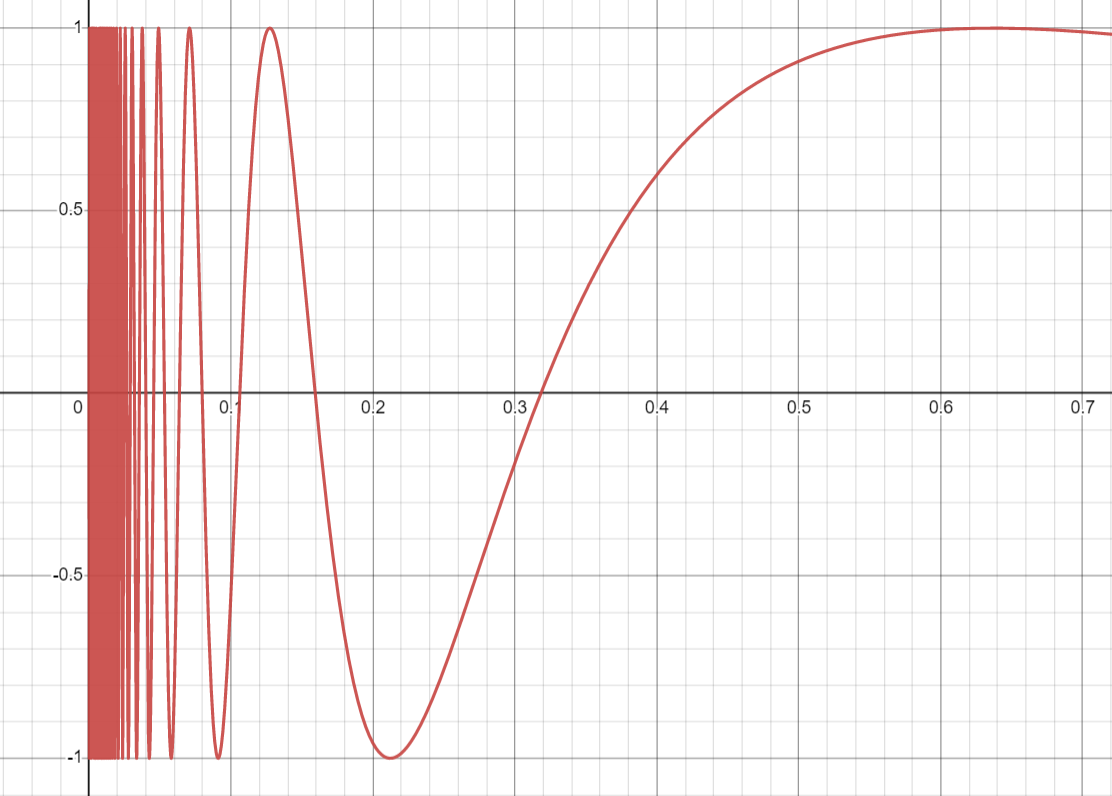
\includegraphics[scale=0.5]{sin.png}
\end{center}


\begin{thm}
Let $\{(X_\alpha,\tau_\alpha) \mid \alpha \in \mathcal{J}\}$ be a set of connected topological spaces, $\prod_{\alpha \in \mathcal{J}}X_\alpha$ is connected when equipped with the product topology. 
\end{thm}
\begin{proof}
The infinite case is left for exercise. For the case where $\mathcal{J}$ is finite, we can proceed by induction.
\end{proof}

\remark In the settings of Theorem 11.4, if $|\mathcal{J}|$ is infinite and $\prod_{\alpha \in \mathcal{J}}X_\alpha$ is equipped with the box topology $\square$, then $(\prod_{\alpha \in \mathcal{J}}X_\alpha, \square)$ is usually disconnected.\\

\example Consider $\mathcal{J} = \Z$, and $X_\alpha = \R$ for $\alpha \in \mathcal{J}$. Define the following sets: 
$$A = \{(x_n) \mid (x_n) \text{ is a bounded sequence}\} \qquad B = \{(x_n) \mid (x_n) \text{ is a unbounded sequence}\}$$
For $x \in A$, we can define $U = \{(y_n) \mid |x_n - y_n| <1\} = \prod_{n \in \Z}B_1(x_n) \subseteq A$, hence it is immediate that we have $A$ being open in the box topology. 

\newpage
\section[Path Connectivity]{\color{red} Path Connectivity\color{black}}
\begin{defn}
Let $(X,\tau)$ be a topological space. $X$ is said to be path connected provided that for all $x,y\in X$, there exists $f:[0,1] \to X$ that is continuous and $f(0) = x$ and $f(1) = y$, where we equip $[0,1]$ with the subspace topology inherits from the Euclidean topology on $\R$. 
\end{defn}

\begin{prop}
Let $(X,\tau)$ be a topological space. If $X$ is path connected, then  $X$ is connected. 
\end{prop}
\begin{proof}
Suppose that we can write $X = A\sqcup B$ for $A,B$ being closed in $X$, we also assume that $X$ is path connected. Suppose also that we have $a\in A$ and $b \in B$, then there exists $f:[0,1] \to X$ with $f(0) = a$ and $f(1) = b$. Note that $A\cap f([0,1])$ is closed, and hence $f^{-1}(A\cap f([0,1]))$ is closed in $[0,1]$ as $f$ is continuous. Similarly, we also know that $f^{-1}(B \cap f([0,1]))$ is closed in $[0,1]$. Note that $X = A\sqcup B$, then we have:
$$[0,1] = f^{-1}(A\cap f([0,1])) \sqcup f^{-1}(B\cap f([0,1])) $$
But $[0,1]$ is connected, hence we must have either $A$ or $B$ being empty, which implies that we have $ X$ being connected, the result follows.
\end{proof}



\example Consider the map $f:(0,1) \to \R^2 \ \ \ t\mapsto (t,\sin(1/t))$. By Theorem 11.3, we know that $A = f((0,1))$ is connected, and hence $\bar{A} = A\sqcup B$ is also connected where we have $B =\{0\}\times [0,1]$. But $\bar{A}$ is not path connected. We can pick $a \in A$ and $b \in B$, and suppose there exists a continuous map $g:[-1,1]\to \bar{A}$ such that $g(-1) = a$ and $g(1) = b$. Here we take:
\begin{align*}
c = \inf\{t \in [-1,1] \mid g(t)\in B\}
\end{align*}
Note that we have $-1<c$. By rescaling $g$, we can assume $c = 0$. Then we can write: 
$$g:[-1,0] \to A\cup \{(0,s) \mid -1\leq s\leq 1\}$$ 
We can pick a sequence $(t_n)$ of points $t_n\in [-1,0]$ such that $(t_n)$ approaches $0$ and $g(t_n) = (x_n, (-1)^n)$. Since $g$ is continuous, then $g(t_n)$ converges to some point, but clearly $(g(t_n))_{n\geq 1} = ((x_n, (-1)^n))_{n\geq 1}$ does not converge to any point, and hence the result follows.

\begin{defn}
Let $(X,\tau)$ be a topological space. $X$ is locally connected at $x \in X$ provided that, for all open neighborhood $U$ of $x$, there exists open neighborhood $V$ of $x$ such that $V\subseteq U$ and $V$ is connected.
\end{defn}

\begin{defn}
Let $(X,\tau)$ be a topological space. $X$ is locally path connected at $x \in X$ provided that for all open neighborhood $U$ of $x$, there exists an open neighborhood $V$ of $x$ such that $V \subseteq U$ and $V$ is path connected. 
\end{defn}

\note Connectivity of a space $X$ does not imply local connectivity for all $x \in X$. Path connectivity of a space $Y$ does not imply local path connectivity for all $y \in Y$. The two statements can be observed from the $f:(0,1) \to \R^2 \ \ \ t\mapsto (t,\sin(1/t))$ example. 


\begin{lem}
Let $(X,\tau)$ be a topological space, and let $\{V_\alpha \mid \alpha \in \mathcal{J}\}$ be a collection of path connected subsets of $X$ such that $\bigcap_{\alpha \in \mathcal{J}}V_\alpha \neq \emptyset$, then $\bigcup_{\alpha \in \mathcal{J}}V_\alpha$ is path connected.
\end{lem}
\begin{proof}
Let $a,b \in \bigcup_{\alpha \in \mathcal{J}}V_\alpha$. Then there exists $\alpha,\beta \in \mathcal{J}$ such that $a \in V_\alpha$ and $b \in V_\beta$. Since $\bigcap_{\alpha\in \mathcal{J}}V_\alpha \neq \emptyset$, there exists $c \in V_\alpha \cap V_\beta$. Hence there exists continuous maps:
\begin{align*}
&f_\alpha :[0,1] \to V_\alpha \qquad\qquad \text{with }f_\alpha(0) = a, \ f_\alpha(1) = c \\
&f_\beta :[1,2] \to V_\beta \qquad\qquad \text{with }f_\beta(1) = c, \ f_\beta(2) = b 
\end{align*}
Now consider the function defined by the following:
\begin{align*}
f:[0,2] \to V_\alpha \cup V_\beta\qquad t\mapsto \begin{cases} 
f_\alpha(t) & t \in [0,1]\\
f_\beta(t) & t\in [1,2]
\end{cases}
\end{align*}
By the Pasting Lemma, we know that $f$ is continuous, and hence this shows that $\bigcup_{\alpha \in \mathcal{J}}V_\alpha$ is path connected. 
\end{proof}

\begin{defn}
Let $(X,\tau)$ be a topological space. A path component containing $x \in X$ is the largest path connected $U \subseteq X$ that satisfies $x \in U$. That is, $U$ is a path component of $x \in X$ provided that for all path connected sets $V \subseteq X$ that contains $x$, we have $V\subseteq U$.
\end{defn}

\begin{lem}
Let $(X,\tau)$ be a topological space. If $X = \bigsqcup_{\alpha \in \mathcal{J}}P_\alpha$ for some path components $P_\alpha$ of $X$, and if $X$ is locally path connected, then each $P_\alpha$ is open.
\end{lem}
\begin{proof}
Let $x \in P_\alpha$, suppose $P_\alpha$ is contained in some open set $V \subseteq X$. Since $X$ is locally path connected, then we know that there exists $U\subseteq V$ containing $x$ such that $U$ is open in $X$, and is path connected. Since $P_\alpha $ is a path component containing $x$, then $U\subseteq P_\alpha$, and $P_\alpha$ is therefore a union of open sets. Hence $P_\alpha $ is also open in $X$. 
\end{proof}




\begin{thm}[Theorem 25.5 on Munkres]
Let $(X,\tau)$ be a topological space. If $X$ is connected and locally path connected, then $X$ is path connected. 
\end{thm}
\begin{proof}
First we can write $X = \sqcup_{\alpha \in \mathcal{J}}P_\alpha$ for some path components $P_\alpha$. Since $X$ is connected and locally path connected, then we know that $P_\alpha$ are open. Since $P_\alpha $ are also disjoint, and $X$ is connected, then we require $P_\alpha = \emptyset$ for all $\alpha$ except a single $\alpha_0 \in \mathcal{J}$, hence $X$ is path connected. That is $X = P_{\alpha_0}$. 
\end{proof}



\remark For a topological space $(X,\tau)$, $X$ can be decomposed into connected components $X_n$, that is $X= \sqcup_{n}X_n$. Each connected $X_n$ can be further decomposed into path connected components $Y_\alpha$, that is $X_n = \sqcup_\alpha Y_\alpha$. Theorem 12.1 states that if $X$ is local path connected, then we have $X_n = Y_{\alpha_0}$, that is path connected components are also connected components. 


\newpage
\chapter{Compactness}
\setcounter{section}{12}

\section[Compact Spaces]{\color{red}Compact Space\color{black}}
\begin{defn}
Let $(X,\tau)$ be a topological space, a collection $\{U_\alpha\subseteq X \mid \alpha \in \mathcal{J}, \ U_\alpha \in \tau\}$ of open subsets of $X$ is called an open cover of $X$ provided that we have $\bigcup_{\alpha \in \mathcal{J}}U_\alpha = X$. 
\end{defn}

\begin{defn}
Let $(X,\tau)$ be a topological space. $X$ is said to be compact provided that for any open cover $\{U_\alpha \mid \alpha \in \mathcal{J}\}$ of $X$, there exists a finite index set $\mathcal{I} \subseteq \mathcal{J}$ such that $\bigcup_{i \in \mathcal{I}}U_i = X$. 
\end{defn}

\begin{thm}[Theorem 26.2 on Munkres]
Let $(X,\tau)$ be a compact topological space. If $A\subseteq X$ is closed, then $A$ is compact. 
\end{thm}
\begin{proof}
Let $\mathcal{U} =\{U_\alpha \mid \alpha \in \mathcal{J}\}$ be an open cover of $A$. Then there exists a collection $\mathcal{V} =\{V_\alpha \mid \alpha \in \mathcal{J}\}$ of open sets in $X$ that satisfies $V_\alpha \cap A = U_\alpha$. Hence we know that $\{X\setminus A\}\cup\mathcal{V}$ is an open cover of $X$. Since $X$ is compact, then we know that $\{X\setminus A\}\cup\mathcal{V}$ admits a finite subcover. That is, there exists $\{V_{\alpha_1}, V_{\alpha_2},\cdots, V_{\alpha_N}, X\setminus A\} $ that covers covers $X$, and hence $\{U_{\alpha_1}, U_{\alpha_2},\cdots, U_{\alpha_N} \}$ covers $A$. This completes the proof.
 \end{proof}

\begin{lem}[Lemma 26.4 on Munkres]
Let $(X,\tau)$ be a topological space. Given $x \in X$, let $A\subseteq X\setminus \{x\}$ be a compact subspace. If $X$ is $T_2$, then there exists open neighborhood $U$ of $x$, and open set $V \in \tau$ that contains $A$  such that $U\cap V = \emptyset$. 
\end{lem}
\begin{proof}
Pick $y \in A\subseteq X$, then there exits disjoint open sets $U_y, V_y$ open in $X$ such that $x \in U_y$ and $y \in V_y$. Note that $A \subseteq \bigcup_{y \in A}V_y$, since $A$ is compact, then there exists finitely many $y_1,y_2,\cdots, y_N \in Y$ such that we have $A \subseteq \bigcup_{n=1}^N V_{y_N}$. Note that $\bigcap_{n=1}^N U_{y_n}$ is an open neighborhood containing $x \in X$, which is disjoint from $V = \bigcup_{n=1}^N V_{y_n}$.
\end{proof}

\begin{thm}[Theorem 26.3 on Munkres]
Let $(X,\tau)$ be a $T_2$ space. If $A\subseteq X$ is compact, then $A$ is also closed.
\end{thm}
\begin{proof}
Pick $x \in X\setminus A$, by Lemma 13.1.1, there exists open sets $U,V$ such that $x \in U$ and $A\subseteq V$, with $U\cap V =\emptyset$. Hence we see that $U \subseteq X\setminus A$. This shows that $X\setminus A$ must be open and hence $A$ is closed.
\end{proof}


\example Let $\R$ be equipped with the cofinite topology, denote such space as $\R_f$. Note that the space $\R_f$ is $T_1$. The only closed subsets of $\R_f$ are finite sets, but every $A\subseteq \R_f$ is compact. Let $A\subseteq \R_f$ be a infinite set, and let $\{W_\alpha \mid \alpha \in \mathcal{J}\}$ be an open cover of $A$. Pick $W_\beta$ for some $\beta \in \mathcal{J}$, we see that $(\R\setminus W_\beta) \cap A = \{x_1,x_2,\cdots, x_N\}$. Then for all $1\leq n \leq N$, we can find some $\alpha_n\in \mathcal{J}$ such that $x_n \in W_{\alpha_n}$, and hence $\{W_\beta, W_{\alpha_1},W_{\alpha_2},\cdots, W_{\alpha_N}\}$ forms a finite open cover of $A$, which implies that $A$ is a compact space. \\


\begin{thm}[Thoerem 26.5 on Munkres]
Let $(X,\tau_X)$ and $(Y,\tau_Y)$ be topological spaces. If $f:X \to Y$ is a continuous map, then for compact subspace $A\subseteq X$, $f(A)$ is a compact subspace of $Y$. 
\end{thm}
\begin{proof}
Suppose $\{U_\alpha \mid \alpha \in \mathcal{J}\}$ is an open cover of $f(A)$. Then $\{f^{-1}(U_\alpha)\mid \alpha \in \mathcal{J}\}$ is an open cover of $A$ as $f$ is continuous. Then we can find a finite index set $\mathcal{I}\subseteq \mathcal{J}$ such that $\{f^{-1}(U_\beta) \mid \beta \in \mathcal{I}\}$ is a finite subcover covering $A$. Hence $\{U_\beta \mid \beta \in \mathcal{I}\}$ is a finite subcover covering $f(A)$. This completes the proof. 
\end{proof}


\begin{thm}
Let $(X,\tau_X)$ and $(Y,\tau_Y)$ be topological spaces, and let $f:X\to Y$ be a bijective continuous map. If $X$ is compact and $Y$ is $T_2$, then $f$ defines a homeomorphism. 
\end{thm}
\begin{proof}
We want to show that $f$ is a closed map. Let $A \subseteq X$ be a closed set, then $A$ is compact, so $f(A)$ is compact, and hence $f(A)$ is closed. This shows that $f^{-1}$ is continuous, hence we conclude that $f$ is a homeomorphism.
\end{proof}

\newpage
\section[Local Compactness]{\color{red}Local Compactness\color{black}}
Suppose that $(X,\tau)$ is a topological space. We want to investigate whether or not there exists a compact space $(\hat{X},\hat{\tau})$ with an embedding $X \to \hat{X}$. In general, $\hat{X}$ does exist but its properties are usually unsatisfying. Thus one wants to put reasonable restrictions on $X$ such that $\hat{X}$ is more reasonable.\\

\begin{defn}
Let $(X,\tau)$ be a topological space. $X$ is said to be locally compact at $x \in X$ provided that there exists a compact subspace $C\subseteq X$, and a neighborhood $U$ of $x$, such that we have $x \in U \subseteq C$. $X$ is said to be locally compact provided that $X$ is locally compact at every $x \in X$. 
\end{defn}

\begin{lem}[Theorem 29.2 on Munkres]
Let $(X,\tau)$ be a Hausdorff space. $X$ is locally compact if and only if for all $x \in X$ and for neighborhood $U$ of $x$, there exists a neighborhood $V$ of $x$ such that $\bar{V}$ is compact and $\bar{V}\subseteq U$. 
\end{lem}


\begin{defn}
Let $(X,\tau)$ be a topological space. $X$ is said to be LCH provided that $X$ is locally compact Hausdorff. 
\end{defn}

\example $\R^n$ equipped with the Euclidean topology is LCH.\\

\example $\Q\subseteq \R$ equipped with the subspace topology inherits from the Euclidean topology on $\R$ is not locally compact.\\

\example $\Z\subseteq \R$ equipped with the subspace topology inherits from the Euclidean topology on $\R$ is LCH.\\

\begin{thm}
Let $(X,\tau)$ be a LCH topological space. We define the one-point compactification of $X$ by $(\hat{X},\hat{\tau})$, where $\hat{X}\coloneqq X\sqcup \{\infty\} $, and $\hat{\tau} \coloneqq \tau \sqcup\{\hat{X}\setminus C \mid C\subseteq X \text{ is compact}\}$, such that $i:X \to \hat{X} \ \ \ x\mapsto x$ is an embedding and $\hat{X}$ is compact.
\end{thm}
\begin{proof}
It is easy to check that $(\hat{X},\hat{\tau})$ is a topological space. To check that $i$ defines an embedding, it suffices to check that $i$ is continuous. Let $\hat{U}\in \hat{\tau}$, then we have either (1) $\hat{U} \subseteq X$, which is open, or (2) $\hat{U} = \hat{X}\setminus C$ for some $C \subseteq X$ being compact. In case (2), since $C$ is compact in $X$, then $C$ is closed in the Hausdorff space $X$, hence we know that $X\setminus C$ is open in $X$, and we have $i^{-1}(\hat{U}) =  X\setminus C = X\cap (\hat{X}\setminus C)$, which is therefore open. This shows that $i$ is an embedding. Now we will show that $\hat{X}$ is compact. Let $\mathcal{U} = \{\hat{U}_\alpha\mid \alpha \in \mathcal{J}\}$ be an open cover of $\hat{X}$. Then there exists $\hat{U}_0$ for some $0 \in\mathcal{J}$ that contains $\infty$. So we know that $\hat{U}_0 = \hat{X} \setminus C$ where $C \subseteq X$ is compact. Moreover $\mathcal{U}\setminus \{\hat{U}_0\}$ is an open cover of $C$, and $C$ is compact in $X$, that is  we obtain a finite cover $\{\hat{U}_1,\hat{U}_2,\cdots, \hat{U}_m\}$ of $C$, and hence $\{\hat{U}_1,\hat{U}_2,\cdots, \hat{U}_m\} \cup \{\hat{U}_0\}$ is a finite cover of $\hat{X}$. This completes the proof. 
\end{proof}

\newpage
\begin{thm}
Let $(X,\tau)$ be a topological space. Then $X$ is LCH if and only if $X$ can be embedded as an open subset of a compact Hausdorff space.  
\end{thm}
\begin{proof}
The $\Rightarrow$ direction is trivial as it follows from Theorem 14.1. For the $\Leftarrow$ direction, let $X$ be the open subset of the compact space $\hat{X}$. Given that $x \in X$, $\hat{X}$ is compact implies $\hat{X}$ is locally compact at $x$. By Lemma 14.0.1, there exists a neighborhood $V$ of $x$ with $\bar{V} \subseteq X$ and $\bar{V}$ being compact. Hence $X$ is locally compact. Moreover, since $X \subseteq \hat{X}$ and $\hat{X}$ is $T_2$, then $X$ is also $T_2$. 
\end{proof}


\example Consider the real line $\R$ equipped with the Euclidean topology. One can \textit{pick} the point $\infty$ as any point in $\R$. The local basis for the topology on  $\hat{\R}$ at $\infty$ takes the form:
\begin{align*}
\{(\R \setminus [a,b]) \cup \{\infty\} \mid a,b \in \R\}
\end{align*}
It is easy to see that $\hat{\R} \cong S^1 \subseteq \R^2$. With similar argument, $\hat{\R^2} \cong S^2 \subseteq \R^3$.\\

\example For $X = \R \sqcup \R$, $\hat{X}$ takes form of two loops connected by a point $\infty$.\\

\example For $\N\subseteq \R$, it is trivial that we have $\N \cong \{1/n \mid n \in \N \} \subseteq \R$. \\
In fact, we also have $\hat{\N} \cong \{1/n \mid n \in \Z \} \cup \{0\}$. \\

\begin{thm}
Let $(X,\tau_X)$ be an LCH space, and let $(Y,\tau_Y)$ be a $T_2 $ compact space such that there exists an embedding $i:X \to Y \ \ \ x\mapsto x$. If $Y \setminus X = \{y_0\}$, then $Y$ is homeomorphic to $\hat{X}$
\end{thm}
\begin{proof}
Let $h:Y \to \hat{X}$ be defined by $h(y) = h(i(x)) = x$ for $y \in i(X)$, and $h(y_0) = \infty \in \hat{X}$. If $U \subseteq Y$ is an open set which does not contain $y_0$, then we see that $i^{-1}(U)$ is open in $X$, and hence $(h\circ i) (U) \subseteq X \subseteq \hat{X}$ is open in $\hat{X}$. Now let $U \subseteq Y$ be a neighborhood of $y_0$, then $Y\setminus U \subseteq X \subseteq Y$ is closed and hence is also compact, then $h(Y\setminus U) \subseteq X \subseteq \hat{X}$ is then compact and closed. This suffices to complete the proof. 
\end{proof}

\newpage
\section[The Tychonoff's Theorem]{\color{red}The Tychonoff's Theorem\color{black}}
Statement of the \textbf{Tychonoff's Theorem}:\\
\textit{Let $\{(X_\alpha,\tau_\alpha) \mid \alpha \in \mathcal{J}\}$ be a family of compact spaces. \\Then $\prod_{\alpha \in \mathcal{J}}X_\alpha$ equipped with the product topology is compact. }\\


Before proving the Tychonoff's Theorem, we want to reformulate compactness in terms of closed sets.

\begin{defn}
Let $(X,\tau)$ be a topological space, and let $\mathcal{C}$ be a collection of subsets of $X$. $\mathcal{C}$ is said to have a fintie intersection property, or FIP, provided that for all $C_1,C_2,\cdots, C_N \in \mathcal{C}$, we have $\bigcap_{i=1}^N C_i \neq \emptyset$. 
\end{defn}

\begin{prop}
Let $(X,\tau)$ be a topological space. $X$ is compact if and only if, for any FIP collection $\mathcal{C}$ of closed subsets of $X$, we have $\bigcap_{C\in \mathcal{C}}C \neq \emptyset$. 
\end{prop}
\begin{proof}
We proceed by contradiction, note that $X$ is not compact if and only if there exists an open cover $\mathcal{U} = \{U_\alpha \mid \alpha \in \mathcal{J}\}$ that has no finite subcover, if and only if for all $U_{\alpha_1}, U_{\alpha_2}, \cdots, U_{\alpha_N}$ with $\alpha_1,\alpha_2,\cdots, \alpha_N \in \mathcal{J}$, we have $\bigcup_{i=1}^N U_{\alpha_i} \neq X$, if and only if we have $\bigcap_{i=1}^N (X\setminus U_{\alpha_i}) \neq \emptyset$ and $\bigcup_{\alpha \in \mathcal{J}}U_\alpha = X$. Hence we have found a desired FIP collection for the contradiction of the proof. This completes the proof.
\end{proof}

Here we motivate the proof of the Tychonoff's Theorem by considering topological spaces $(X_1,\tau_1)$ and $(X_2,\tau_2)$, and their product. Let $\mathcal{C}$ be a FIP collection of closed subsets of $X_1\times X_2$. Here it is true that $\{\Pi_1(C) \mid C\in \mathcal{C}\}$ is a FIP collection of subsets of $X_1$. Note that $\Pi_1$ is not a closed map, that is $\Pi_1(C)$ is not necessarily closed in $X_1$. For example, $C = \{(x,y) \in \R^2 \mid xy=1 \}$ is a closed subset of $\R^2 \times \R^2$, but $\Pi_1(C ) = \R \setminus \{0\}$ is open and not closed. \\

Now consider the following problem, suppose we have the following holds:
\begin{align*}
x_1 \in \bigcap_{C \in \mathcal{C}} \overline{\Pi_1(C)} \qquad\qquad\qquad x_2 \in \bigcap_{C \in \mathcal{C}}\overline{\Pi_2(C)}  \tag{*}
\end{align*}
however, the following is not necessarily true given that (*) holds:
\begin{align*}
(x_1,x_2) \in \bigcap_{C \in \mathcal{C}}C
\end{align*}
Here is a counterexample, suppose the intersection of sets in $\mathcal{C}$ is the line segment $L=\{(x,y) \mid 0\leq x\leq 1, x=y\}$. The projection of $C\in \mathcal{C}$ on $\R$ contains the interval $(0,1)$, but $(1/19, 1/29) \notin L$. \\

The idea is that we want to restrict our \textit{choice} of picking elements in the intersection of the projections. To do this, we need to make use of the Zorn's Lemma, which is equivalent to the Axiom of Choice. \\


\begin{defn}
Let $(A,<)$ be a partially ordered set, $x \in A$ is a maximal element of $A$ provided for all $y \in A$ with $y \neq x$, we have either $y<x$, or $x$ and $y$ being not comparable. 
\end{defn}

\begin{lem}[Zorn's Lemma]
Let $(A,<)$ be a partially ordered set. If for all $S\subseteq A$ that is totally ordered, there exists $s \in A$ that is an upper bound for $S$, that is, for all distinct $x,y \in S$, we have either $x<y\leq s$ or $y<x \leq s$. Then there exists a maximal element $x$ in $A$.
\end{lem}

\begin{lem}[Lemma 37.1 on Munkres]
Let $(X,\tau)$ be a topological space. We define the following set:
\begin{align}
\mathcal{Z} = \{\mathcal{A}\mid \mathcal{A} \text{ is a FIP family of subsets of }X\}
\end{align}
$\mathcal{Z}$ admits a maximal element when regarded as a partially ordered set under set inclusion. 
\end{lem}
\begin{proof}
Suppose $S\subseteq \mathcal{Z}$ is a totally ordered set. We will show that $\bigcup_{\mathcal{A} \in S}\mathcal{A} \in \mathcal{Z}$ is a FIP. Suppose we have $A_1,A_2,\cdots, A_N \in \bigcup_{\mathcal{A} \in S}\mathcal{A}$, then there exists $\mathcal{A}_1,\mathcal{A}_2,\cdots, \mathcal{A}_N \in S$ such that $A_i \in \mathcal{A}_i$. WLOG, we suppose $\mathcal{A}_N \supseteq \mathcal{A}_{N-1} \supseteq \cdots \supseteq \mathcal{A}_1$. Since $\mathcal{A}_N$ is FIP, then we must have $\bigcap_{i=1}^N A_i \neq \emptyset$. Hence this completes the proof via Zorn's Lemma. 
\end{proof}

The next step is to investigate the maximal FIP collection. 
\begin{lem}[Lemma 37.2 on Munkres]
Let $(X,\tau)$ be a topological space, and let $\mathcal{Z}$ be defined by (3.1). Denote $\mathcal{D} \in \mathcal{Z}$ as the maximal element of $\mathcal{Z}$. Then we have the followings hold:
\begin{enumerate}[topsep=3pt,itemsep=-1ex,partopsep=1ex,parsep=1ex]
\item For $D_1,D_2,\cdots, D_N \in \mathcal{D}$, we have $\bigcap_{i=1}^N D_i \in \mathcal{D}$.
\item For any $U \subseteq X$, if $U\cap D \neq \emptyset$ for all $D \in \mathcal{D}$, then $U \in \mathcal{D}$.
\end{enumerate}
\end{lem}
\begin{proof}
We will show (1) first. Here we fix $D_1,D_2,\cdots, D_N \in \mathcal{D}$, and let $B = \bigcap_{i=1}^ND_i$, we will show that $\{B\} \cup \mathcal{D}$ is a FIP. Suppose that $A_1,A_2,\cdots, A_m \in \mathcal{D}$, then we can write the following as $\mathcal{D}$ is a FIP:
\begin{align*}
B\cap A_1 \cap A_2 \cap \cdots \cap A_m = D_1 \cap D_2 \cap \cdots \cap D_N \cap A_1 \cap A_2 \cap \cdot \cap A_m \neq \emptyset
\end{align*}
Hence we see that $\{B\}\cup \mathcal{D}$ is a FIP. This completes the proof of (1). Now for (2), we want to show that $\{U \} \cup \mathcal{D}$ is a FIP. For $D_1,D_2,\cdots, D_N \in \mathcal{D}$, by (1) we know that $D_1\cap D_2\cap \cdots \cap D_N \in \mathcal{D}$, then we can write:
\begin{align*}
U \cap D_1 \cap D_2 \cap \cdots \cap D_N \neq \emptyset \qquad \Rightarrow \qquad U \in \mathcal{D}
\end{align*}
This completes the proof of the lemma. 
\end{proof}


\begin{thm}[The Tychonoff's Theorem]
Let $\{(X_\alpha,\tau_\alpha) \mid \alpha \in \mathcal{J}\}$ be a family of compact spaces. \\Then $\prod_{\alpha \in \mathcal{J}}X_\alpha$ equipped with the product topology is compact.
\end{thm}
\begin{proof}
Let $\mathcal{D}$ denote the maximal FIP family of subsets of $X$. Here we want to find $x \in \bigcap_{D\in \mathcal{D}}\overline{D}$, then the result of the Theorem follows from Proposition 15.0.1. Note that: 
$$\Pi_\alpha(\mathcal{D}) = \{ \Pi_\alpha (D) \mid D\in \mathcal{D}\} \text{ is a FIP family on }X_\alpha$$ 
The compactness of $X_\alpha$ implies that there exists $x_\alpha \in \bigcap_{D\in \mathcal{D}}\overline{ \Pi_\alpha(D)}$. Let $x = (x_\alpha)_{\alpha \in \mathcal{J}} \in X$, let $U_\alpha$ be an open neighborhood of $x_\alpha$, and consider the open set $\Pi_\alpha^{-1}(U_\alpha) \subseteq X$ which contains $x$. If $D \in \mathcal{D}$, we see that the following holds by construction:
\begin{align*}
x_\alpha \in \left( U_\alpha \cap \overline{\Pi_\alpha (D)}\right)
\end{align*}
W++e have either $x_\alpha \in \Pi_\alpha(D)$, or $x_\alpha$ is a limit point of $\Pi_\alpha(D)$, that is, there exists $y_\alpha \in U_\alpha \cap \Pi_\alpha(D)$. Either way, we see that $\Pi_\alpha(D) \cap U_\alpha \neq \emptyset$, so $D \cap \Pi_\alpha^{-1}(U_\alpha) \neq \emptyset$. Then Lemma 15.0.4 part (2) implies that $\Pi_\alpha^{-1}(U_\alpha) \in \mathcal{D}$, and by Lemma 15.0.4 part (1), we see that finite intersection of $\Pi_\alpha^{-1}(U_\alpha)$ belongs to $\mathcal{D}$. That is, any open set containing $x$ is in $\mathcal{D}$. Now let $U$ be an open neighborhood of $x$, here $U \in \mathcal{D}$, we also let $D \in \mathcal{D}$ be arbitrary. Then we have $U\cap D \neq \emptyset$ by the FIP property of $\mathcal{D}$, hence we have $x \in \bar{D}$, and hence $x \in \bigcap_{D\in \mathcal{D}}\bar{D}$. This completes the proof. 
\end{proof}

\newpage
\section[Compactification]{\color{red} Compactification\color{black}}
\begin{defn}
A space $(Y,\tau_Y)$ is called a compactification of the space $(X,\tau_X)$ provided that $Y$ is a compact Hausdorff space and there exists an embedding $i:X \to Y$ such that $\bar{X} = Y$. 
\end{defn}

\example If $(X,\tau)$ is a LCH space, then $\hat{X}$, the one-point compactification of $X$, is a compactification of $X$.\\

\example For the interval $X=(0,1)\subseteq \R$ equipped with the Euclidean topology, the one-point compactification $\hat{X}$ is homeomorphic to $S^1$. Moreover, $Y = [0,1]$ is also a compactification of $X$, in particular, we can embed $i:X \to Y$, and we have $\bar{X} = [0,1]$ in $\R$. 

\begin{prop}
Let $(Z,\tau_Z)$ be a compact and Hausdorff space, and consider there exists an embedding $i:X\to Z$, then $Y = \bar{X}$ is a compactification of $X$.  
\end{prop}  
\begin{proof}
Since $\bar{X}$ can be viewed as a closed subset of a compact Hausdorff space, and hence is compact. This completes the proof. 
\end{proof}

\example Consider $X = (0,1) \subseteq \R$ where we equip $\R$ with the Euclidean topology, and consider the embedding $i:X\to [-1,1]^2 \qquad t\mapsto (t,\sin(1/t))$. Hence we have $\bar{X} \subseteq [-1,1]^2$ is the topologiest sine curve, that is $\bar{X} = i(X)\cup([-1,1]^2 \cap \{(x,y) \mid x = 0\})$. \\

Let $(X,\tau)$ be a topological space. Previously, we saw that if $A\subseteq X$ is Hausdorff, and $f:A \to \R$ is continuous, then there exists a unique continuous extension $g:\bar{A}\to \R$ of $f$. Suppose now $f:X \to \R$ is continuous, we are interested in finding a compactification $Y$ of $X$ such that $f$ extends continuously to $Y$. \\

\example Take $X = (0,1)$ and define $f:X \to \R \ \ \ t\mapsto t$. An appropriate compactification is $[0,1]$ such that $f$ extends continuously to $[0,1]$. However, if one takes $g:X \to \R \ \ \ t\mapsto \sin(1/t)$, we note that there is no continuous extension of $g$ to $[0,1]$. But there does exist a continuous extension for $f$ to some compactification $Y$. Here we use $g$ to embed $X$ into a product of intervals: 
\begin{align*}
h:X \to [-1,1]^2 \qquad t\mapsto (t,g(t))
\end{align*}
then the compactification $Y$ is provided by Proposition 16.0.1, and the projection $f = \pi_2 \circ h$ gives a continuous extension to $Y$. Note that, we require $f$ to be bounded for the product of intervals to be compact, and we can generalize this result to any number of functions.\\

\begin{defn}
Let $(X,\tau)$ be a LCH space, and consider the set of functions:
\begin{align*}
\mathcal{F} = \{f_\alpha : X \to [0,1] \mid \alpha \in \mathcal{J}, \ f_\alpha\text{ is continuous and bounded on }X\}
\end{align*}
Consider the map $f:X \to [0,1]^\mathcal{J} \ \ \ x\mapsto (f_\alpha(x))_{\alpha \in \mathcal{J}}$. First we note here $[0,1]^\mathcal{J}$ is compact by the Tychonoff's Theorem. Here $f$ is an embedding, and $\beta(X) \coloneqq \bar{X} \subseteq [0,1]^\mathcal{J}$ is called the Stone-Cech compactification of $X$. 
\end{defn}
We will show here the $f$ defined in Definition 16.0.1.0.1 is an embedding.
\begin{proof}
First note that $f$ is bijective onto its image. $f$ would fail to be injective if there exists $x ,y\in X$ such that $f_\alpha(x) = f_\alpha	 (y)$ for all $f_\alpha \in \mathcal{F}$. According to Urysohn, there exists a continuous function $g:X \to \R$ such that $g(x) = 1$ and $g(y) = 0$, given that $X$ is LCH. Hence $f$ is injective, and therefore a bijection onto its image. Note that $f$ is continuous and $\pi_\alpha \circ f = f_\alpha$ is continuous for all $\alpha \in \mathcal{J}$. To show that $f$ is open, one can use the fact that there exists a function $g$ such that $g(x) = 1$ and $g(y)= 0$ for $\forall y \in X\setminus U$ where $U$ is a chosen neighborhood of $x$. 
\end{proof}

\begin{prop}
Let $g:X \to [0,1]$ be a continuous function on a topological space $(X,\tau)$. There exists a a continuous extension $\hat{g}$ of $g$ defined by $\hat{g}:\beta(X) \to [0,1]$. 
\end{prop}
\begin{proof}
Note that $g\coloneqq f_\alpha$ for some $f_\alpha \in \mathcal{F}$, so we can consider $\pi_\alpha \circ f = f_\alpha = g$, which defines $\hat{g}$. This completes the proof. 
\end{proof}

\begin{prop}
Let $g:X \to C$ where $C$ is a compact Hausdorff spcae, then $\hat{g}:\beta(X) \to C$ is an embedding extending $g$. 
\end{prop}
\begin{proof}
One can construct an embedding $p:C \to [0,1]^\mathcal{I}$. $p_\beta \circ g : X \to [0,1]$ for any $\beta \in \mathcal{I}$ are contained in $\mathcal{F}$. Using $(g_\beta)_{\beta \in I}:X \to [0,1]^I$ can complete the proof. 
\end{proof}


\newpage
\chapter{Countability and Separability}
\setcounter{section}{16}
\section[Countability Axioms]{\color{red} Countability Axioms\color{black}}
\begin{defn}
A topological space $X$ is said to be first countable provided that it admits a countable local basis at each point $p\in X$. 
\end{defn}

\begin{defn}
A topological space $X$ is said to be second countable provided that it admits a countable basis for the topology.
\end{defn}

\note Clearly, all second countable spaces are first countable.\\

\remark Most metric spaces are not second countable.

\begin{prop}
The followings are true:
\begin{enumerate}[topsep=3pt,itemsep=-1ex,partopsep=1ex,parsep=1ex]
\item A countable product of first countable spaces is first countable. 
\item A countable product of second countable spaces is second countable. 
\item Subspaces of first countable spaces are first countable.
\item Subspaces of second countable spaces are second countable.
\end{enumerate}
\end{prop}

\begin{defn}
Let $(X,\tau)$ be a topological space. $X$ is said to be Lindelof provided that every open cover of $X$ admits a countable subcover. $X$ is said to be separable provided that there exists a countable set $A\subseteq X$ with $\bar{A} = X$, in which case $A$ is said to be dense. 
\end{defn}

\begin{prop}
Let $(X,\tau)$ be a second countable space, then $X$ is Lindelof and separable. 
\end{prop}
\begin{proof}
The proof of $X$ being Lindelof is given on \textit{Munkres} Theorem 30.3. To show that $X$ is separable, let $\{U_n \mid n \in \N\}$ be a countable basis of $X$, and let $A$ be a set defined by picking $x_n \in U_n$ for all $n \in \N$. Suppose $W$ is open, so $x_n \in U_n \subseteq W$ for some $n \in \N$. Let $y \in X$ such that $W$ is a neighborhood of $y$, then $W\cap A  \neq \emptyset$ and hence $y \in \bar{A}$. This suffices to complete the proof. 
\end{proof}

\begin{prop} Consider the real line $\R$ equipped with the lower-limit topology, and denote such space as $\R_l$. Note that $\R_l$ is first countable, Lindelof, separable, but not second countable. 
\end{prop}
\begin{proof}
This is an example in section 30 on \textit{Munkres}, for details of the proof, check out explanations on \textit{Munkres}. To show that $\R_l$ is first countable, consider the intervals $U_n = [x, x+1/n)$. To show that $\R_l$ is separation, one can make use of $\Q \subseteq \R$. To show that $\R_l$ is not second countable, suppose $\mathcal{B}$ is a basis for the lower-limit topology on $\R$, given $x \in \R_l$, pick $U_x\in \mathcal{B}$ which is contained in $[x,x+1)$ and contains $x$, so if $x \neq y$, then $U_x \neq U_y$ as we have $\inf(U_y) = x$ while $\inf(U_y) = y$. Hence we conclude that $\mathcal{B}$ is not countable. 
\end{proof}

\example $\R_l^2$ is not Lindelof. To show that, consider $L = \{(x,-x) \mid x \in \R\} \subseteq \R_l^2$. It is not hard to see that $L$ is closed in $\R_l^2$, hence $\R^2 \setminus L$ is open in $\R_l^2$. Consider the box $U_y = [y, y+1) \times [-y, -y+1)$, note that the cover $(\R^2\setminus L)\sqcup\{U_y\mid y \in \R_l\}$ does not have countable subcovers.


\newpage
\section[Separation Axioms]{\color{red}Separation Axioms \color{black}}
\begin{defn}
Let $(X,\tau)$ be a topological space. $X$ is said to be $T_0$ provided that for all $x,y \in X$, there exists $U\in \tau$ with either $x \in U$ with $y \notin U$, or $x \notin U$ with $y \in U$. $X$ is said to be $T_1$ provided that for all $x,y \in X$, there exists $U \in \tau$ with $x \in U$ and $y \notin U$. $X$ is said to be $T_2$ provided that for all $x,y \in X$, there exists $U,V \in \tau$ such that $x\in U$, $y \in V$, and $U \cap V = \emptyset$. A $T_2$ space is called a Hausdorff space. \\

$X$ is said to be $T_3$ provided that, $X$ is $T_1$, and for all $x \in X$, and all closed sets $A \subseteq X$ that does not contain $x$, there exists disjoint $U,V \in \tau$ such that $x \in U$ and $A\subseteq V$. A $T_3$ space is called a regular space.\\

$X$ is said to be $T_4$ provided that, $X$ is $T_1$, and for all $A,B \subseteq X$ that are closed and disjoint, there exists disjoint $U,V \in \tau$ with $A \subseteq U$ and $B \subseteq V$. A $T_4$ space is called a normal space. 
\end{defn}


\begin{lem}
Let $(X,\tau)$ be a $T_1$ space. Then the followings hold:
\begin{enumerate}[topsep=3pt,itemsep=-1ex,partopsep=1ex,parsep=1ex]
\item $X$ is regular if and only if for all $x \in X$ and all neighborhood $U$ of $x$, there exists an open set $V$ containing $x$ with $\bar{V} \subseteq U$. 
\item $X$ is normal if and only if for all $A \subseteq X$ that is closed, and all $U \in \tau$ that contains $A$, there exists $V \in \tau$ with $A \subseteq V$ and $\bar{V} \subseteq U$. 
\end{enumerate}
\end{lem}
\begin{proof}
For statement (1), we first consider the $\Rightarrow$ direction. Let $x \in X$, and let $U$ be a neighborhood of $x$. Note that $X \setminus U = A$ is closed, so there exists $W,V \in \tau$ that are disjoint with $x\in V$ and $A\subseteq W$. By the fact that for all $a \in A$, $W$ is a neighborhood of $a$ disjoint from $V$, so $\bar{V}\subseteq U$. For the $\Leftarrow$ direction of (1), take $x \in X$, and $A\subseteq X$ be closed that does not contain $x$. Then we know that $X\setminus A = U$ is open, and $x \in U$, so we can find open set $V$ such that $x \in V \subseteq \bar{V} \subseteq U$, then $W = X\setminus \bar{V}$ contains $A$ and disjoint from $V$. This completes the proof of (1). The proof of (2) is similar.
\end{proof}


\begin{prop}
Subspaces of regular spaces and arbitrary products of regular spaces are regular.
\end{prop}
\begin{proof}
Let $(X,\tau)$ be a regular space. If $Y \subseteq X$ is equipped with subspace topology, it is immediate that $Y$ is $T_1$. Furthermore, we can pick $x \in Y$, and $x \notin A \subseteq Y$ such that $A$ is relatively closed, then there exists $B \subseteq X$ that is closed with $A = B\cap Y$ and $x \notin B$. Since $X$ is regular, one can find disjoint open sets $U,V \subseteq X$ such that $x \in U$ and $B \subseteq V$, and we obtain the desired relative open set $U\cap Y$ that contains $a$ and disjoint from $A$. Now consider $X = \prod_{\alpha \in \mathcal{J}}X_\alpha$ is a product of regular spaces $X_\alpha$. It is immediate that $X$ is $T_1$. Let $x= (x_\alpha)_{\alpha \in \mathcal{J}}$ be contained in an open set $U \subseteq X$. One can pick a basis element $W = \Pi_{\alpha_1}^{-1}(W_{\alpha_1})\cap \Pi_{\alpha_2}^{-1}(W_{\alpha_2})\cap \cdots \cap \Pi_{\alpha_n}^{-1}(W_{\alpha_n}) \subseteq U$ that contains $x$, with $W_{\alpha_{i}} \subseteq X_{\alpha_i}$ being open. Then by Lemma 18.0.1, there exists $V_{\alpha_i}$ being open in $X_{\alpha_i}$ with $x_{\alpha_i}\in V_{\alpha_i}$ and $\overline{V}_{\alpha_i} \subseteq W_{\alpha_i}$. Consider the set $V =\bigcap_i \Pi_{\alpha_i}^{-1}(V_{\alpha_i})$, which contains $x$. Note that $\Pi_{\alpha}^{-1}(V_\alpha) = \prod_{\alpha'}K_{\alpha'}$ where $K_{\alpha'} = X_{\alpha'}$ for $\alpha' \neq \alpha$ and $K_\alpha = V_\alpha$. Then it is not hard to see that $\overline{\Pi_{\alpha}^{-1}(V_\alpha)} = \prod_{\alpha'}\overline{K_{\alpha'}}$, and it follows that we have $\overline{V} = \bigcap_{i=1}^n\Pi_{\alpha_i}^{-1}(\overline{V}_{\alpha_i}) \subseteq U$ is closed. This suffices to complete the proof by Lemma 18.0.1.
\end{proof}


\example The real line equipped with the lower-limit topology, $\R_l$, is a $T_4$ space. To show that, let $A,B \subseteq \R$ be closed disjoint sets, then we can define:
\begin{align*}
U = \bigcup_{a \in A}[a,x_a) \qquad\qquad\qquad V = \bigcup_{b \in B}[b, y_b)
\end{align*}
where we choose $x_a $ such that $[a,x_a) \subseteq \R\setminus B$ for all $a \in A$. Similarly, we pick $y_b$ such that $[b,y_b) \subseteq \R\setminus A$ for all $b \in B$. One can show that $U \cap V = \emptyset$. Moreover, $U,V$ are open and contain $A,B$ respectively, hence that completes the result. \\

\example $\R_l^2$ is not a $T_4$ space. As shown previously in Section 17 of this text, the subspace topology equipped on $L = \{(x,-x) \mid x \in \R\} \subseteq \R_l^2$ is the discrete topology. Hence any subset of $L$ is closed in $\R_l^2$ as $L$ is also closed. Making use of subsets of $L$ completes the proof, details are shown on \textit{Munkres} Section 31. 

\newpage
\section[Normal Spaces]{\color{red}Normal Spaces\color{black}}
\begin{thm}[Theorem 32.1 on Munkres]
Let $(X,\tau)$ be a second countable $T_3$ space, then $X$ is $T_4$. 
\end{thm}
\begin{proof}
Let $A,B\subseteq X$ be disjoint closed sets. Let $x \in A$, then $X\setminus B$ is an open neighborhood of $x$. By Lemma 18.0.1, since $X$ is $T_3$, then we know that there exists $V\in \tau$ such that $x \in V$ and $\bar{V} \subseteq X\setminus B$. Here we can pick $\mathcal{B} = \{U_n' \mid n \in \N\}$ that is a countable basis of $X$. Pick $U_n\in \mathcal{B}$ with $x \in U_n \subseteq \bar{U}_n\subseteq \bar{V}\subseteq  X\setminus B$. In such a way we get a countable cover $\mathcal{U} = \{U_n \mid n \in \N\}$ of $A$ with $\bar{U}_n \cap B = \emptyset$. Similarly, we can construct a countable open cover $\mathcal{V} = \{V_n \mid n \in \N\}$ of $B$ with $\bar{V}_n \cap A = \emptyset$. Here we define:
\begin{align*}
\that{U}_n = U_n \setminus \bigcup_{i=1}^n \overline{V}_n
\qquad\qquad\qquad 
\that{V}_n = V_n \setminus \bigcup_{i=1}^n \overline{U}_n
\end{align*}
note that $\that{U}_n$ is open as $U_n$ is open and $\bigcup_{i=1}^n \overline{V}_n$ is closed, and $\that{\mathcal{U}} = \{\that{U}_n \mid n \in \N\}$ is still a cover of $A$. Similarly, $\that{V}_n$ is open and $\that{\mathcal{V}} = \{\that{V}_n \mid n \in \N\}$ is still a cover of $B$. Set $U = \bigcup_{n}\that{U}_n$, which is open containing $A$, and $V = \bigcup_n \that{V}_n$, which is open containing $B$. If there exists $x \in U \cap V$, then there exists $n,m$ with $x \in \that{U}_n\cap \that{V}_m \subseteq U_n \cap \that{V}_m  = \emptyset$, a contradiction, and that completes the proof.   
\end{proof}


\begin{thm}[Theorem 32.2 on \textit{Munkres}]
Metrizable spaces are $T_4$ spaces. 
\end{thm}
\begin{proof}
Let $(X,d)$ be a metric space equipped with the topology induced by metric $d$. Let $A,B \subseteq X$ be disjoint closed sets. For $a \in A$, let $\epsilon_a >0$ such that $B_{\epsilon_a}(a) \subseteq X\setminus B$, and similarly, pick $\delta_b >0$ for $b \in B$ with $B_{\delta_b}(b)$. Here we take $U = \bigcup_{a \in A}B_{\epsilon_a/19}(a)$ and $V = \bigcup_{b \in B} B_{\delta_b/19}(b)$. Clearly, $U,V$ are open and $A \subseteq U$ and $B \subseteq V$. To show that $U$ and $V$ are disjoint, suppose we have $x \in U \cap V$, then there exists $a\in A$ and $b \in B$ with $x \in B_{\epsilon_a/19}(a)\cap B_{\delta_b/19}(b)$, but then the following must be satisfied:
\begin{align*}
d(a,b) \leq d(a,x) + d(x,b) \leq \frac{\epsilon_a}{19} + \frac{\delta_b}{19} \leq \max\{\epsilon_a,\delta_b\}
\end{align*}
hence we must have either $b \in B_{\epsilon_a}(a)$ or $b \in B_{\delta_b}(b)$, which gives us a contradiction, and therefore completes the proof. 
\end{proof}

\begin{thm}[Theorem 32.3 on \textit{Munkres}]
Compact Hausdorff spaces are $T_4$ spaces. 
\end{thm}
\begin{proof}
Let $X$ be a compact space. Via Lemma 13.1.1, if $x \in X$, and $A\subseteq X$ is a compact subset such that $x \notin A$, then there exists disjoint open sets $U,V \subseteq X$ such that $x \in U$ and $A\subseteq V$, that is, we see here $X$ is a $T_3$ space. Now let $A,B \subseteq X$ be disjoint closed sets. For $a \in A$, we use the $T_3$ property of $X$ to find open disjoint sets $U_a$, $V_a$ such that $a \in U_a$ and $B \subseteq V_a$. Clearly, $\{U_a\mid a \in A\}$ is a cover of $A$. Here we choose a finite subcover of $A$, $\{U_{a_1}, U_{a_2},\cdots, U_{a_N}\}$, along with the corresponding family $\{V_{a_1}, V_{a_2},\cdots, V_{a_N}\}$. in which case we have $U = \bigcup_{i=1}^N U_{a_i}$ and $V = \bigcap_{i=1}^NV_{a_i}$ as the desired open sets.
\end{proof}

\example $\R^\mathcal{J}$ is not normal if the index set $\mathcal{J}$ is uncountable. Note however $\R^{\mathcal{J}}$ is regular by Proposition 18.0.2. \\

\example Given an index set $\mathcal{J}$, we note that $\R^{\mathcal{J}}$ is homeomorphic to $(0,1)^{\mathcal{J}}$. $[0,1]^\mathcal{J}$ is compact Hausdorff by the Tychonoff's Theorem, and hence is $T_4$ by Theorem 19.3, however, $(0,1)^{\mathcal{J}}$, as a subspace of $[0,1]^\mathcal{J}$, is not normal. Then we see here subspace of a normal space is not necessarily normal.

\newpage
\section[Completely Regular Spaces]{\color{red}Completely Regular Spaces\color{black}}
\begin{thm}[Urysohn's Lemma]
Let $X$ be a normal space, and let $A,B\subseteq X$ be disjoint closed sets. There exists a continuous function $f:X \to [0,1]$ with $f(a) = 0$ for all $a\in A$ and $f(b)=1$ for all $b \in B$. 
\end{thm}
\remark In the settings of Theorem 20.1. $A\subseteq f^{-1}([0,1/2))$ and $B \subseteq f^{-1}((1/2, 1])$. 
\begin{proof}[Proof of Theorem 20.1]
Here we will construct open subsets $U_p \subseteq X$ labeled by $p \in P = \Q \cap [0,1]$, such that, for $p<q$, we have $\bar{U}_p \subseteq U_q$. First we fix an enumeration of $P$ such that $1$ and $0$ are the first two elements on the enumeration. Let $U_1 = X\setminus B$. By the normality of $X$, there exists open $U_0$ such that $A \subseteq U_0 \subseteq \bar{U}_0 \subseteq X\setminus B = U_1$. Let $P_n$ be the set of the first $n$-elements in the enumeration of $P$, and suppose $r \in P$ is the $(n+1)$-st element on the enumeration of $P$, note that there exists $p,q \in P_n$ with $p<r<q$ where $q =\min\{s \in P_n \mid s>r\}$ and $p = \max\{t \in P_n \mid t<r\}$. By induction, we have $\bar{U}_p \subseteq U_q$, so by normality, there exists $U_r$ with $\bar{U}_p \subseteq U_r \subseteq \bar{U}_r \subseteq U_q$.\\

Next, we construct the desired function $f$ as the following:
\begin{align*}
f:X \to \R \qquad x\mapsto \begin{cases}
\inf\{p \in P \mid x \in U_p \} & x \in U_1\\
1 & x\in B
\end{cases}
\end{align*} 
Given $r$, if $x \in \bar{U}_r$, then $f(x) = \inf\{p \in P \mid x \in U_p\}\leq r$ as we have $\bar{U}_r \subseteq U_p$ for any $p>r$. If $x \notin U_r$, then $x \notin U_p$ for any $p<r$, then $f(x) \geq r$. \\

Here we will check the continuity of $f$. Fix $(c,d) \subseteq [0,1]$, if we pick any $x \in X$ that satisfies $f(x) \in (c,d)$, we want to find an neighborhood $U\subseteq X$ containing $x$ with $f(U) \subseteq (c,d)$, that is $x \in U \subseteq f^{-1}((c,d))$. Pick $p,q \in P$ with $c<p< f(x) < q< d$, and we consider $U = U_q \setminus \bar{U}_p$. We want to show that $x \in U$ and $f(U) \subseteq (c,d)$. Since $f(x) >p$, we have $x \notin \bar{U}_p$ by argument above, and since $f(x) <q$, we have $x \in U_q$ by argument above, hence we conclude that $x \in U$. Since $U \subseteq U_q$, then $f(U) \leq q$, and since $U \cap \bar{U}_p  = \emptyset$, then we see that $f(U) \geq p$, hence we conclude that $f(U )\subseteq (c,d)$. This suffices to complete the proof of the theorem.  
\end{proof}


\begin{defn}
A topological space $(X,\tau)$ is said to be completely regular, or $T_{3.5}$, provided that for all $x \in X$ and all $A \subseteq X$ that is closed and $x \notin A$, there exists a continuous function $f:X \to [0,1]$ with $f(x) = 1$ and $f(A) = 0$. 
\end{defn}

\remark A $T_{4}$ space is a $T_{3.5}$ space by Theorem 20.1.2 

\begin{thm}
Subspaces of $T_{3.5}$ spaces and arbitrary products of $T_{3.5}$ spaces are $T_{3.5}$. 
\end{thm}
\begin{proof}
Let $Y$ be a subset of a $T_{3.5}$ space $X$. For $x \in Y$, and $A \subseteq Y$ be a relatively closed set that does not contain $x$. Note that there exists a closed set $B \subseteq X$ such that $A = B \cap Y$ with $x \notin B$. Hence there exists $f:X \to [0,1]$ with $f(x) = 1$, and $f(B) =0$, then $f|_Y$ is the desired continuous function that we want. The proof of products of $T_{3.5}$ spaces being $T_{3.5}$ is given on \textit{Munkres} Theorem 33.2.   
\end{proof}

\begin{defn}
Let $(X,\tau)$ be a topological space. A collection $\mathcal{F} = \{f_\alpha \mid \alpha \in \mathcal{J}\}$ of continuous functions, with index set $\mathcal{J}$, defined by $f_\alpha :X \to [0,1]$, is said to be separating points from closed sets provided that for all $x \in X$, and any closed set $A\subseteq X$ that does not contain $x$, there exists $f_\alpha\in \mathcal{F}$ with $f_\alpha(x) = 1$ and $f_\alpha(A) = 0$. Conventionally we say that such a collection $\mathcal{F}$ is separating.
\end{defn}

\begin{thm}
Let $(X,\tau)$ be a $T_1$ space. If there exists a separating collection of continuous functions $\mathcal{F} = \{f_\alpha\mid \alpha \in \mathcal{J}\}$, then $F:X \to [0,1]^{\mathcal{J}} \ \ \ x\mapsto (f_\alpha(x))_{\alpha \in \mathcal{J}}$ is an embedding of $X$ into $[0,1]^\mathcal{J}$. 
\end{thm}
\begin{proof}
Note that $F$ is continuous as $\Pi_\alpha \circ F = f_\alpha$ is continuous. Moreover, $F$ is injective, as we see that for $x,y \in X$ with $x \neq y$, then there exists $f_\alpha\in \mathcal{F}$ such that $f_\alpha(x) = 1$ and $f_\alpha(y) = 0$ as $X$ is $T_1$, hence $F(x) \neq F(y)$. Now set $Z = F(X)$, for open set $U \subseteq X$, we want to show that $F(U) \subseteq Z$ is relatively open. Pick $z \in F(U)$, since $F$ is injective, then there exists $x \in X$ with $f(x) = z$, that is $x \in U$. Now there exists $\alpha \in \mathcal{J}$ with $f_\alpha(x) = 1$ and $f_\alpha(X\setminus U)  =0$. Define $V = \Pi_\alpha^{-1}((0,1])$, which is open in $[0,1]^{\mathcal{J}}$, and set $W = V\cap Z$, which is relatively open in $Z$, then we claim that $z \in W$ and $W \subseteq F(U)$. Note that $\Pi_\alpha(z) = \Pi_\alpha(F(x)) = f_\alpha(x)=1$, hence $z \in V$. Now pick $y \in W$, we can find $b \in X$ with $F(b) = y$, where we see that $\Pi_\alpha(y) = \Pi_\alpha(F(b)) = f_\alpha(b) > 0$ by the definition of $W = V\cap Z = \Pi_\alpha^{-1}((0,1]) \cap Z$, and hence $b \in U$. This proves that $F$ is an open map.  
\end{proof}


\begin{corT}
Let $(X,\tau)$ be a topological space. $X$ is $T_{3.5}$ if and only if there exists embedding of $X$ into $[0,1]^{\mathcal{J}}$ for some index set $\mathcal{J}$. 
\end{corT}
\begin{proof}
The $\Rightarrow$ direction is given by Theorem 20.3. For the $\Leftarrow$ direction, we note that $[0,1]^\mathcal{J}$ is a $T_4$ space, and hence is $T_{3.5}$, then we see that $X$ is also a $T_{3.5}$ space. 
\end{proof}

\note $[0,1]^{\mathcal{J}}$ is metrizable if $\mathcal{J}$ is countable. 


\begin{thm}[Urysohn's Metrization Theorem]
Let $(X,\tau)$ be a second countable $T_3$ space, $X$ is metrizable.  
\end{thm}
\begin{proof}
Note that $X$ is $T_4$ by Theorem 19.1. Also note that $\R^{\mathcal{J}}$ is metrizable when $\mathcal{J}$ is countable. Here we want to find countable separating family of continuous functions on $X$, in which case a homeomorphism can be defined between $X$ and a subspace of the metrizable space $\R^{\mathcal{J}}$ by Theorem 20.3. Let $\mathcal{B} = \{U_n \mid  n \in \N\}$ be a countable basis for the topology $\tau$ on $X$. For $n,m \in \N$ that satisfies $\bar{U}_n \subseteq U_m$, by Urysohn's Lemma, there exists $g_{nm}:X \to [0,1]$ with $g_{nm}(\bar{U}_n)  = 0$, and $g_{nm}(X\setminus U_m)=1$. Consider the following definition:
\begin{align*}
\mathcal{C} = \{g_{nm} \mid \bar{U}_n \subseteq U_m, \ \text{choose a particular }g_{nm}\text{ as a representation}\}
\end{align*}
Note here $\mathcal{C}$ is countable. Given closed $A\subseteq X$, for $x \in X\setminus A = U$, since $\mathcal{B}$ is a basis, then there exists $m \in \N$ such that $x \in U_m \subseteq U$. Since $X$ is $T_3$, there exists open $V$ with $x \in V \subseteq \bar{V} \subseteq U_m$, and again, there exists $n \in \N$ such that $x \in \bar{U}_n \subseteq \bar{V} \subseteq U_m$. Now one can find $g_{nm}$ with $g_{nm}(\bar{U}_n) = 0$ and $g_{nm}(X\setminus U_m) = 1$. Hence we conclude that we have $g_{nm}(x) = 0$ and $g_{nm}(A) = 1$. This suffices to prove the theorem as $\mathcal{C}$ is the desired countable separating family of continuous functions. 
\end{proof}


\newpage
\chapter{The Fundamental Group}
\setcounter{section}{20}
\section[Homotopy]{\color{red}Homotopy\color{black}}
\begin{defn}
Let $(X,\tau_X)$ and $(Y,\tau_Y)$ be topological spaces, and let $f:X \to Y$ and $g:X\to Y$ be continuous maps. A homotopy between $f$ and $g$ is a continuous map $F:X \times I \to Y$, where $I = [0,1]$, that satisfies $F(x,0) = f(x)$ and $F(x,1) = g(x)$ for all $x \in X$. If such a homotopy $F$ between $f$ and $g$ exists, then $f$ and $g$ are said to be homotopic.  \footnote{In this chapter, if not specified otherwise, $I$ is taken to be the interval $I = [0,1]$.}
\end{defn}

\begin{defn}
Let $(X,\tau)$ be a topological space, a continuous map $f:I \to X$ is called a path in $X$. 
\end{defn}

\begin{defn}
A function $f$ is said to be nulhomotopic provided that $f$ is homotopic to a constant map. 
\end{defn}

\example Consider $S^1$ and $Y = \R^2 \setminus \{(0,0)\}$. The identity map $i:S^1 \to Y \ \ \ x\mapsto x$ is not nulhomotopic, as one cannot \textit{shrink} the image of $i$ using a continuous map to a single point without crossing the origin $(0,0) \in \R^2$, which is not contained in $Y$. 

\begin{defn}
Let $(X,\tau_X)$ be a topological space, let $f:I \to X$, $g:I \to X$  be continuous functions with $f(0) =g(0) = x_0$, $f(1) = g(1) = x_1$. A function $F:I\times I\to X$ is called a path homotopy between $f$ and $g$ provided that $F$ is a homotopy between $f$ and $g$ such that $F(0,s) = x_0$ for all $t \in I$ and $F(1,s) = x_1$ for all $s \in I$. 
\end{defn}

\begin{prop}
The homotopic relation between functions defines a equivalence relation, denoted as $\simeq$. Path homotopic relation between functions also defines a equivalence relation, denoted as $\simeq_p$. 
\end{prop}
\begin{proof}
Here we will show that homotopy defines a equivalence relation. Consider topological spaces $(X,\tau_X)$ and $(Y,\tau_Y)$. It is not hard to see that $f:X \to Y$ is homotopic to $f$ as the homotopy $F$ defined by $F(x,t) \coloneqq f(x)$ is a continuous function on $X \times [0,1]$. Suppose now $f$ is homotopic to $g$, with homotopy $F$. Then $G(x,t) \coloneqq F(x,1-t)$ is a homotopy from $g$ to $f$, that is $g$ is also homotopic to $f$. Furthermore, suppose now $f:X\to Y$ is homotopic to $g:X\to Y$, and $g$ is homotopic to $h:X\to Y$, by homotopies $F$ and $G$, respectively. Here we construct a function $H:X\times I \to Y$:
\begin{align*}
H(x,t) = \begin{cases}
F(x,2t) & t \in [0,1/2]\\
G(x,2(t-1/2)) & t \in [1/2, 1]
\end{cases}
\end{align*}
Here $H$ is well defined as we have $F(x,1) = g(x) = G(x,0)$, then it is clear that $H$ is continuous by the pasting lemma, and hence it follows that $H$ defines a homotopy from $f$ to $h$. This completes the proof that homotopy defines a equivalence relation. 
\end{proof}

\begin{defn}
Let $(X,\tau)$ be a topological space, and let $f:I \to X$, $g:I \to X $ be continuous functions that satisfy $f(0)= x_0$, $f(1) = g(0) = x_1$, and $g(1) = x_2$. Here we define $(f*g):I \to X$ to be a path from $x_0$ to $x_2$:
\begin{align*}
(f*g)(t) \coloneqq \begin{cases}
f(2t) & t \in [0,1/2]
\\
g(2t-1 ) & t \in [1/2,1]
\end{cases}
\end{align*}
\end{defn}

\begin{defn}
Let $(X,\tau)$ be a topological space, and let $f:I \to X$, $g:I \to X$ be continuous functions, such that $f(1) = g(0)$, write $[f] $ as the eqiuivalence class of of path homotopies of $f$. We define $[f*g]\coloneqq [f]*[g]$.
\end{defn}

Here we want to verify Definition 21.0.1.0.2. Given the settings in the definition, suppose that $f_1 \in [f]$ and $g_1\in [g]$, let $F, G$ be path homotpopies from $f$ to $f_1$, and from $g$ to $g_1$, respectively. Consider the function $H$ defined by: 
\begin{align*}
H(t,s) = \begin{cases}
F(t, 2s) & s \in [0,1/2] \\ 
G(t, 2s-1) & s \in [1/2,1]
\end{cases}
\end{align*}
We see that $H$ is a homotopy hence $f*g$ is homotopic to $f_1*g_1$.\\

\begin{defn}
Let $(X,\tau)$ be a topological space, and let $x_0 \in X$. A path $f:I \to X$ is called a loop at $x_0$ provided that $f(0) = f(1) = x_0$.\end{defn}

\remark It is obvious that the $*$-product of loops is well defined.

\begin{thm}
Let $(X,\tau)$ be a topological space, and let $x_0 \in X$. 
Consider $G_{x_0} = \{[f] \mid f\text{ is a loop at }x_0\}$. $(G_{x_0},*)$ is a group.
\end{thm}
\begin{proof}
Here we want to check the associativity for $[f], [g],[h]\in G_{x_0}$:
\begin{align*}
[f] *([g]*[h]) = ([f]*[g]) *[h]
\end{align*}
and we need to find the identity $[e]\in G_{x_0}$ and find the inverse for $[f]\in G_{x_0}$. Here we will first find the identity in this group. Consider $[e] \coloneqq [c]$, where $c:I \to X \ \ \ t\mapsto x_0$. It is not hard to verify that the following function defines a homotopy between loop $f$ at $x_0$ and $f*e$:
\begin{align*}
F(t,s) = \begin{cases}
f((2-s) t) & t \in [0,1/(2-s)] \\
f(1) & t \in [1/(2-s), 1]
\end{cases}
\end{align*} 
Another way of constructing the homotopy between $f$ and $f*e$ is given by:
\begin{align*}
F(s,t) = \begin{cases}
f(2t/(1+s)) & t \in [0,(s+1)/2]\\
f(1) & t\in [(s+1)/2, 1]
\end{cases}
\end{align*}
Similarly we can construct homotopy from $f*e$ to $f$, that suffices to show that $e$ is the identity in the group.\\ 

For inverse of $[f]$, here we define $g:[0,1]\to X \ \ \ x\mapsto f(1-t)$. To show that $g$ is an inverse of $f$, it is not hard to see that the following function defines a homotopy between $f*g$ and $e$:
\begin{align*}
F(t,s)  = \begin{cases}
f(2t) & t\in \left[0,(1-s)/2\right]\\
f\left(-2t(1-s)/(1+s) + 2(1-s)/(1+s) \right) & t \in [(1-s)/2, 1] \end{cases}
\end{align*}
Another homotopy to consider here is:
\begin{align*}
F(t,s) = \begin{cases}
f(2t) & t \in [0,(1-s)/2]\\
f(1-s) & t \in [(1-s)/2, (s+1)/2]\\
f(2(1-t)) & t \in [(s+1)/2, 1]
\end{cases}
\end{align*}
Similarly, we have $g*f$ homotopic to $e$. This suffices to show that $g$ is an inverse of $f$ in the group. In the rest of the text, if not specified otherwise, we denote the inverse of $f$ in the group $(G_{x_0}, *)$ as $\overline{f}$.\\

For the associativity, we want to show that $([f]*[g])*[h] = [f]*([g]*[h])$, where we can consider the following homotopy:
\begin{align*}
F(t,s) = \begin{cases}
f(4t/(s+1)) & t\in [0,(s+1)/4]\\
g(4(t-(s+1)/4)) & t \in [(s+1)/4, (s+2)/4]\\
h( 4 (t-(s+2)/4)/(2-s) ) & t \in [(s+2)/4 , 1]
\end{cases}
\end{align*}
This completes the proof. 
\end{proof}

\remark Theorem 51.2 on \textit{Munkres} is a generalized version of Theorem 21.1 for paths instead of loops. 

\begin{thm}
Let $f:I \to X$ be a loop at $x_0$ in a topological space $(X,\tau)$, and let $0 < a_0 < a_1<\cdots<a_{n-1}<a_n = 1$. Consider $L_i$ to be the linear map that satisfies $L_i(0) =a_{i-1}$ and $L_i(1) = a_i$, and the functions $f_i \coloneqq f\circ L_i$, which are paths from $f(a_{i-1})$ to $f(a_i)$. Then we have $[f] = [f_1]*[f_2]*\cdots*[f_n]$. 
\end{thm}
\begin{proof}
We can proceed by induction, the $n=1$ is trivial. Now suppose we have the case for $n-1$ holds, let $g = [f_1]*[f_2]*\cdots*[f_{n-1}]$, which is a path from $x_0$ to $f(a_{n-1})$, then we are left to show $[f] = [g]*[f_n]$. The rest of the proof is left for the reader. 
\end{proof}

\begin{defn}
Let $(X,\tau)$ be a topological space. The fundamental group of $X$ relative to the base point $x_0 \in X$ is defined by $\pi_1(X,x_0) \coloneqq \{[f]\mid f:I \to X\text{ is a loop at }x_0\}$. 
\end{defn}

\example $\pi_1(\R^n , x_0) = \{[e_{x_0}]\}$. To verify that, we need to show that for all loop $f$ at $x_0$, we have $[f] = [e_{x_0}]$. Here we can consider the homotopy $F(t,s) = sx_0 + (1-s) f(t)$.

\begin{defn}
A set $X\subseteq \R^n$ is said to be convex provided that for $x,y \in X$, the straight line $L  = \{(1-t)x + ty \mid t \in [0,1]\}$ lies entirely in $X$. 
\end{defn}

\example Consider $x_0 \in B^n \coloneqq \{ x \in \R^n \mid x_1^2 + x_2^2 + \cdots +x_n^2 \leq 1\} $, we have $\pi_1(B^n, x_0) = 0$, where $0$ here denote the trivial group $\{[e_{x_0}]\}$. Similarly, any convex subset $X$ of $\R^n$ satisfies $\pi_1(X,x_0) = 0$. \\

\example $\pi(S^1,x_0)$ is isomorphic to $(\Z,+)$.  \\

\begin{thm}
Let $(X,\tau)$ be a topological space, and let $\alpha:I \to X$ be a path in $X$ from $x_0$ to $x_1$. Then $\alpha$ induces a group homomorphism:
\begin{align*}
\hat{\alpha}: \pi_1(X,x_0) \to \pi_1(X,x_1) \qquad [f] \mapsto [\bar{\alpha}]*[f]*[\alpha]
\end{align*}
where $\bar{\alpha}: I \to X \ \ \ t\mapsto \alpha(1-t)$. 
\end{thm}
\begin{proof}
It is not hard to check that $\hat{\alpha}$ is a group homomorphism, as for $[f],[g] \in \pi_1(X,x_0)$, we have the following holds by associativity of $*$:
\begin{align*}
\hat{\alpha} \left( [f] *[g]\right)  = [\bar{\alpha}]*[f]*[g]*[\alpha] = [\bar{\alpha}]*[f]*[\alpha]*[\bar{\alpha}] * [g] * [\alpha] = \hat{\alpha}\left( [f]\right) * \hat{\alpha}\left([g]\right)
\end{align*}
Showing that $\hat{\alpha}$ is well-defined completes the proof. 
\end{proof}
\begin{corT}
$\hat{\alpha}$ defined in Theorem 21.3 is a group isomorphism. 
\end{corT}
\begin{proof}
Here we denote the inverse of $\alpha$ as $\beta$ and consider a similar definition of $\hat{\beta}$. We want to show that $\hat{\alpha}(\hat{\beta}([h])) = [h]$ and $\hat{\beta}(\hat{\alpha}([f])) = [f]$. The proof is given in Theorem 52.1 on \textit{Munkres}. 
\end{proof}

\begin{corL}
Let $(X,\tau)$ be a path connected topological space, $\pi_1(X,x)$ is isomorphic to $\pi_1(X,y)$ for all $x,y \in X$.  
\end{corL}

\begin{defn}
A topological space $(X,\tau)$ is said to be simply connected provided that $X$ is path connected and $\pi_1(X,x)$ is the trivial group for all $x \in X$. 
\end{defn}
\begin{lem}
Let $(X,\tau)$ be a simply connected topological space, let $f,g$ be paths connecting $x,y \in X$, then $[f] = [g]$.
\end{lem}
\begin{proof}
Consider $\bar{g}:I \to X \ \ \ t\mapsto g(1-t)$, and consider $[f]*[\bar{g}]$, which forms a loop at $x$. That is, we have $[f] * [\bar{g}]$ is the identity element in $\pi_1(X,x)$, then we see here $[f]*[\bar{g}]*[g] = [f] = [e]*[g] = [g]$. This completes the proof. 
\end{proof}



\example Let $U \subseteq \R^n$ be a convex set, and let $f:I \to U$, $g:I \to U$ be two paths satisfying $f(0) = g(0) = x$ and $f(1) = g(1) = y$, then we can construct a straight line homotopy: 
$$F: I \times I \to U\qquad (t,s)\mapsto (1-s) f(t) - tg(t)$$
Then it is not hard to see from here that any convex set is simply connected.\\

\example $S^2 \subseteq \R^3$ is simply connected.

\begin{prop}
Let $U,V$ be simply connected subsets of a topological space $(X,\tau)$. If $U\cap V$ is path connected, then $U \cup V$ is simply connected. 
\end{prop}

\begin{defn}
Let $h:X\to Y$ be a continuous function between topological spaces $(X,\tau_X)$ and $(Y,\tau_Y)$ that sends $x_0 \in X$ to $h(x_0) = y_0 \in Y$. The group homomorphism associated to $h$ at the base point $x_0$ is defined by:
\begin{align*}
h_* : \pi_1(X,x_0) \to \pi_1(Y,y_0) \qquad [\alpha] \mapsto [h\circ \alpha]
\end{align*}
\end{defn}
Here we will check that the homomorphism in Definition 21.3.3.0.1 is well-defined:
\begin{proof}
Here we can write:
\begin{align*}
h_*([\alpha]) * h_*([\beta]) = [h\circ \alpha] * [h\circ \beta] = [h\circ (\alpha*\beta)] = h_*([\alpha]*[\beta])
\end{align*}
which completes the proof. 
\end{proof}

\begin{prop}
Let $(X,\tau_X)$, $(Y,\tau_Y)$, and $(Z,\tau_Z)$ be topological spaces, and let $h:X \to Y$, $k:Y \to Z$ be continuous functions that satisfy $h(x_0) = y_0 $ and $k(y_0) = z_0$. Then we have $(k\circ h)_* = (k_*\circ h_*): \pi_1 (X,x_0) \to \pi_1(Z,z_0)$.  Furthermore, if $i:X \to X \ \ \ x\mapsto x$ is the identity map on $X$, then $i_*$ is the identity homomorphism on $\pi_1(X,x)$ for all $x \in X$.
\end{prop}
\begin{proof}
Here we can write the following:
\begin{align*}
(k\circ h)_*([\alpha]) = [k\circ h\circ \alpha] = k_*([h\circ \alpha]) = k_*(h_*([\alpha])) = (k_*\circ h_*)[\alpha]
\end{align*}
For all $[\alpha]\in \pi_1(X,x_0)$. 
\end{proof}

\begin{corT}
If $h:X \to Y$ is a homeomorphism between topological spaces $(X,\tau_X)$ and $(Y,\tau_Y)$, then $\pi_1(X,x_0)$ is isomorphic to $\pi_1(Y,h(x_0))$ for all $x_0 \in X$. 
\end{corT}


\newpage
\section[Covering Space]{\color{red}Covering Space\color{black}}
\begin{defn}
Let $(E,\tau_E)$ and $(B,\tau_B)$ be topological spaces and let $p:E \to B$ be a continuous surjective map. Let $U \subseteq B$ be an open set, $U$ is said to be evenly covered by $p$ provided that $p^{-1}(U) = \bigsqcup_{\alpha \in \mathcal{J}}V_\alpha$ for open sets $V_\alpha \subseteq E$, and $p|_{V_\alpha}$ is a homeomorphism onto $U$. The sets $V_\alpha$ are called the slices of $p^{-1}(U)$. 
\end{defn}

\begin{defn}
Let $(E,\tau_E)$ and $(B,\tau_B)$ be topological spaces and let $p:E \to B$. $p$ is called a covering map provided that for all $x \in B$, there exists open $U\subseteq B$ such that $x \in U$ and $U$ is evenly covered by $p$. $E$ is called a covering space of $B$ provided that $p$ is a covering map.
\end{defn}

\example Given a topological space $(E,\tau)$, $E$ is a covering space of itself, and the covering map can be taken to be the identity transformation.\\

\example For topological space $(B,\tau)$, we can define $E = B \times A$, where $A$ is a discrete set. Then we can take $p $ to be the projection map as the covering map:
\begin{align*}
p^{-1}(U) = \bigsqcup_{\alpha \in A} V_\alpha \qquad \text{with }V_\alpha = U\times \{\alpha\}
\end{align*}

\example For $E = \R$ and $B = S^1$, we can take $p(t) = (\cos(2\pi t), \sin(2\pi t))$ and show that $p$ is a covering map, that is $E$ is a covering space of $B$. \\


\example 
Consider $B = E = S^1$, we consider $p$ as the doubling map:
\begin{align*}
p:E \to B \qquad	 (\cos(s),\sin(s)) \mapsto (\cos(2s), \sin(2s))
\end{align*}
here $p$ is again a covering map. \\

\example $E = (0,\infty) \subseteq \R$, and let $B =S^1\subseteq \R^2$. Note that the following map does not define a covering map:
\begin{align*}
p:E \to B \qquad t\mapsto (\cos(2\pi t), \sin(2\pi t))
\end{align*}
For an open neighborhood $U$ of $(1,0) \in S^1$, by considering $p^{-1}(U)$, one can show that $(1,0)$ is not covered evenly by $p$.\\


\begin{defn}
Let $(X,\tau_X)$ and $(Y,\tau_Y)$ be topological spaces. A map $f:X \to Y$ is a local homeomorphism provided that for all $y \in Y$ and any $x \in f^{-1}(\{y\})$, there exists a neighborhood $U$ of $y$ and a neighborhood $V$ of $x$ such that $f|_V$ is a homeomorphism onto $U$.  
\end{defn}


\begin{prop}
A local homeomorphism is an open map. 
\end{prop}
\begin{proof}
Let $f;X \to Y$ be a local homeomorphism between topological spaces $(X,\tau_X)$ and $(Y,\tau_Y)$. Let $W \in \tau_X$, we can denote $y = f(x)$ for $x \in W$. There exists a neighborhood $U$ of $x$ and a neighborhood $V$ of $y$ such that $f|_V: V\to U$ is a homeomorphism. Now we see that $V\cap W \subseteq W$ is open, so we have $f|_V(V\cap W)$ is open in $U$.  Since $U$ is open in $Y$, then $f|_V(V\cap W)$ is open in $Y$ contianing $f(W)$ and $y$, which completes the proof.  
\end{proof}

\begin{prop}
Let $(E,\tau_E)$ and $(B,\tau_B)$ be topological spaces with a covering map $p:E \to B$, let $A$ be a subspace of $B$, then $p|_{p^{-1}(A)}: p^{-1}(A) \to A$ is a covering map. 
\end{prop}


\begin{prop}
Let $(E_i,\tau_{E_i})$ and $(B_i,\tau_{B_i})$ be topological spaces for $i \in \{1,2\}$, with covering maps $p_1:E_1 \to B_1$ and $p_2:E_2 \to B_2$. Then $p_1 \times p_2 : E_1 \times E_2 \to B_1 \times B_2 \ \ \ (m,n)\mapsto (p_1(m),p_2(n))$ is a covering map. 
\end{prop}



\example Consider $p:\R \to S^1 \ \ \ t\mapsto (\cos(2\pi t) ,\, \sin(2\pi t))$, and we consider the product of the map $p$: 
$$p_2 :\R^2 \to S^1 \times S^1 \qquad (s,t) \mapsto (p(s), p(t))$$
Consider the sets $L_1 = \{(t,0) \mid t \in [0,1]\} \subseteq \R^2$, and $L_2 = \{(0,s) \mid s \in [0,1]\} \subseteq \R^2$. Here we see that $p_2(L_1)$ and $p_2(L_2)$ are two loops on the torus $S^1 \times S^1$. We can look at union of the two loops in $S^1 \times S^1$, which is a subspace $A$ of $S^1 \times S^1$. Then $p_2|_{p^{-1}(A)}: p^{-1}(A) \to A$ is a covering map, and the target $A$ can be deformed into a shape ``$\infty$'' of two loops intersecting at a single point. 

\newpage
\section[Liftings]{\color{red}Liftings in Covering Spaces\color{black}}

\begin{defn}
Let $(X,\tau_X)$ and $(Y,\tau_Y)$ be topological spaces. 
Let $\alpha: I \to X$ be a path and let $p:Y \to X$ be a map. A lifting of $\alpha$ by $p$ is a path $\that{\alpha}:I \to Y$ that satisfies $p\circ \that{\alpha} = \alpha$. 
\end{defn}

\example Consider $p : \R \to S^1$ be the usual covering, and a path $\alpha:I \to S^1$ that loops $S^1$ once. Then the image of the lift of $\alpha$ is an interval $[a,b]\subseteq \R$ that satisfies $b-a  = 1$ and $b \in \Z$. If instead we have a path $\beta: I \to S^1$ that loops $S^1$ twice, the lift of $\beta$, denoted as $\that{\beta}$, has an image $[a,b]\subseteq \R$ that satisfies $b-a = 2$ and $b \in \Z$, and additionally satisfying $p(\that{\beta}(1/2)) = (1,0)$, that is $\that{\beta}(1/2) =\in p^{-1}(1,0) \in \Z$. 

\begin{lem}[Lemma 54.1 on \textit{Munkres}]
Let $(X,\tau_X)$ and $(Y,\tau_Y)$ be topological spaces with a covering map $p:Y \to X$, and let $\alpha:I \to X$ be a path in $X$ from $x_0$ to $x_1$. Then for each $y_0 \in p^{-1}(x_0)$, there exists a unique path $\that{\alpha }:I \to Y$ which is a lift of $\alpha$ starting at $y_0$.  
\end{lem}
\begin{proof}
Here we cover $X$ using a set of open sets $\mathcal{U} = \{U_i \mid i \in \mathcal{J}\}$, each of which is evenly covered by $p$. Then one can find a partition of $[0,1]$, with $0=s_0 < s_1 <  \cdots < s_m = 1$, such that $\alpha([s_{i-1}, s_i]) \subseteq U_i$ for some evenly covered relabeled $U_i\in \mathcal{U}$. We inductively define $\that{\alpha}$ lift. Suppose that we have a lift of $\alpha|_{[0,s_{i-1}]}$, where for the base case we define $\that{\alpha}(s_0)=\that{\alpha}(0) = y_0$, then $\alpha([s_{i-1}, s_i])\subseteq U_i$. We pick $V_i $ to be slice of $p^{-1}(U_i)$ which contains $\that{\alpha}(s_{i-1})$. Now we map $\alpha|_{[s_{i-1},s_i]}$ homeomorphically by $p$ to a $\that{\alpha}|_{[s_{i-1},s_i]}$ in $V_i$. By Pasting Lemma, we get a continuous path lifting $\alpha|_{[0,s_i]}$. The proof of uniqueness is given on \textit{Munkres}
\end{proof}

\begin{lem}[Lemma 54.2 and Theorem 54.3 on \textit{Munkres}]Let $(X,\tau_X)$ and $(Y,\tau_Y)$ be topological spaces with a covering map $p:Y \to X$, and let $\alpha,\beta$ be homotopic paths in $X$. If $\that{\alpha}$ and $\that{\beta}$ are the unique lifts starting at $y_0 \in p^{-1}(\alpha(0)) = p^{-1}(\beta(0))$, then $\that{\alpha}$ and $\that{\beta}$ are homotopic. Moreover, if $\alpha$ and $\beta$ are path homotopic, then $\that{\alpha}$ and $\that{\beta}$ are also path homotopic and they end at the same point. 
\end{lem}
\begin{proof}
Suppose $F$ is a homotopy from $\alpha$ to $\beta$, that is $F:I \times I \to X$ satisfies $F(t,1) = \beta(t)$ and $F(t,0) = \alpha(t)$. The proof is based on the use of $F$, as given in \textit{Munkres}. 
\end{proof}

\note Let $(E,\pi_E)$ and $(B,\pi_B)$ be topological spaces with a covering map $p:E \to B$, and with $E$ being path connected. Let $b_0 \in B$ and $e_0, e_1 \in p^{-1}(b_0)$. There exists a path $\alpha$ from $e_0$ to $e_1$, and $p\circ \alpha$ is a loop in $B$ based at $b_0$.  

\begin{thm}[Lifting Correspondence I]
Let $(E,\pi_E)$ and $(B,\pi_B)$ be topological spaces with a covering map $p:E \to B$, and with $E$ being path connected. Let $e_0 \in E$ such that $p(e_0) = b_0$. Then there exists a map $\phi: \pi_1(B, b_0) \to p^{-1}(b_0)$ such that $\phi([\alpha]) \coloneqq \that{\alpha}(1)$ where $\that{\alpha}$ is the lift of $\alpha$ starting at $e_0$. Moreover, $\phi$ is surjective, and if $E$ is simply connected, then $\phi$ is a bijection. $\phi$ is called the lifting correspondence derived from $p$. 
\end{thm}
\begin{proof}
First we will check that $\phi$ is well defined, and we suppose here we have $[\alpha ] = [\beta]$ with $\alpha,\beta$ being loops in $B$ based at $b_0$. Then if $\that{\alpha}, \that{\beta}$ are lifts starting at $e_0$, we require that $\that{\alpha}(1) = \that{\beta}(1)$, but this is just a consequence of Lemma 23.0.2 on liftings of path homotopic functions. Now we will show that $\phi$ is surjective, where we can pick $e_1 \in p^{-1}(b_0)$, we have a path $\alpha$ in $E$ from $e_0$ to $e_1$. Then the loop $p\circ \alpha$ is a loop in $B$ with $\phi([p \circ \alpha]) = e_1$, which gives the result. Moreover, if $E$ is simply connected, we can consider $[f],[g] \in \pi_1(B, b_0)$ with $\phi([f]) = \phi([g])$. In which case $\that{f}$ and $\that{g}$ are paths from $e_0$ to $e_1 = \phi([f])$. Since $E$ is simply connected, we see that $\that{f}$ is path homotopic to $\that{g}$ by a path homotopy $\that{F}$. Then $p \circ \that{F} = F$ is a path homotopy from $f$ to $g$. This completes the proof.
\end{proof}


\begin{thm}[Fundamental Group of $S^1$]
For $x_0 \in S^1$, $\pi_1 (S^1, x_0) $ is isomorphic to $\Z$.
\end{thm}
\begin{proof}
Let $p:\R \to S^1$ be the usual covering map. Consider $x_0 = (1,0)$ where we have $p^{-1}(x_0) = \Z$. Theorem 23.1 implies that there exists bijection $\phi$ between $\pi_1(S^1, x_0)$ and $\Z$. Now it remains to show that $\phi$ is a homomorphism. Suppose $[f],[g] \in \pi_1(S^1,x_0)$, and we denote $0 = e_0 \in p^{-1}(x_0)$. Let $m = \phi([g])$, and $n = \phi([f])$. Let $\that{f}$ and $\that{g}$ be the lifts of $f$ and $g$. We define $\that{h}:I \to \R \ \ \ t\mapsto \that{g}(t) +n$. Then $\that{f} * \that{h}$ is a path from $0$ to $n+m$. It follows from the fact that $(p\circ \that{h})(s) = p(\that{h}(s)) = p(\that{g}(s)+n) = p(\that{g}(s)) = g(s)$ that we have $p\circ (\that{f}*\that{h}) = ( p\circ \that{f}) *(p \circ \that{h})= f*g$. We conclude that $n+m = \phi([f*g]) = \phi([f]) + \phi([g])$, and hence $\phi$ is a isomorphism. 
\end{proof}

%\begin{thm}[Lifting Correspondence II]
%Let $(E,\pi_E)$ and $(B,\pi_B)$ be topological spaces with a covering map $p:E \to B$, and with $E$ being path connected, let $e_0 \in p^{-1}(b_0)$. Then $p_*: \pi_1(E_1,e_0) \to \pi_1(B,b_0)$ is injective monomorphism. Set $H$ to be the image of $p_*$, then $\phi$ induces a bijection: 
%$$\Phi:\pi_1(B, b_0)/H \to p^{-1}(b_0) \qquad [f]H \mapsto \phi([f])$$
%Moreover, if $f$ is a loop in $B$ based at $b_0$, then $[f] \in H$ if and only if $\that{f}$ is a loop in $E$ based at $e_0$. 
%\end{thm}
%\begin{proof}
%Suppose $\that{h}$ is a loop in $E$ at $e_0$, with $p_*([h]) = [e]$ being the identity loop in $\pi_1(B,b_0)$. We have $p\circ \that{h}$ homotopic to the trivial loop, so we can lift ot get a path homotopy from $\that{h}$ to trivial loop at $e_0$. Now we suppose that $f,g$ are loops in $B$ at $b_0$, with $\that{f},\that{g}$ being their lifts. Then $\phi[f] = \phi[g]$ if and only if $[f] \in [g]H$. For the $\Leftarrow$ direction, suppose $[f] \in [g] H$, then $f$ is homotopic to $gh$ for some $[h] \in H$. By definition, there exists a loop $\that{h}$ in $E$ at $e_0$ with $h$ homotopic to $p \circ \that{h}$. Now $\that{g} \that{h}$ is well defined, and one can check that $\that{g}\that{h}$ is a lift for $gh$. Then $\that{f} = \that{g}$, and hence $\that{f}(1) = (\that{g} \that{h})(1) = \that{g} (1)$, which completes the $\Leftarrow$ direction. For the $\Rightarrow$ direction, if $\phi([f]) = \phi([g])$,, then $\that{f}(1) = \that{g} (1)$,, so $[\that{f}] = [\that{g} \circ \overline{\that{g}}\that{f}] = [\that{g}][h]$ for some $[h] \in \Pi_1(E)$, note that $\overline{\that{g}}\that{f}$ is a loop at $e_0$ and hence $[f] \in [g] H$. 
%\end{proof}

\begin{defn}
Let $G$ be a group, and let $H$ be a subgroup of $G$. For $g\in G$, $gH$ is the left coset of $H$ defined by $gH\coloneqq \{gh \mid h \in H\}$. The right coset of $H$ associated to $g$ is defined similarly by $Hg\coloneqq \{hg \mid h \in H\}$
\end{defn}
\remark In the settings of Definition 23.2.0.0.1, usually, there exists distinct $g_1,g_2$ such that $g_1H = g_2H$. Hence the representation of $gH$ is not unique.

\begin{defn}
Let $G$ be a group and let $H$ be a subgroup of $G$, we define $G/H \coloneqq \{ gH \mid g \in G\}$. \\
$H$ is called a normal subgroup of $G$ provided that for all $g \in G$ we have $H = gHg^{-1}$. \\
$G/H$ is called a quotient group provided that $H$ is a normal subgroup of $G$. 
\end{defn}

\begin{prop}
Let $G$ be a group, and let $H$ be a subgroup of $G$. $G/H$ is a group if $H$ is normal. The operation on $G/H$ is defined by $(g_1H)(g_2H) \coloneqq g_1g_2H$ for any $g_1,g_2 \in G$. 
\end{prop}

\begin{thm}[Lifting Correspondence II]
Let $(E,\tau_E)$ and $(B,\tau_B)$ be topological spaces with a covering map $p:E \to B$, let $b_0 \in B$, and $e_0 \in p^{-1}(b_0)$. Define $H = p_*(\pi_1(E,e_0))$. Then we have the followings hold:
\begin{enumerate}[topsep=3pt,itemsep=-1ex,partopsep=1ex,parsep=1ex]
\item $p_*:\pi_1(E,e_0) \to \pi_1(B,b_0)$ is injective.
\item If $E$ is path connected, $\Phi:\pi_1(B,b_0)/H \to p^{-1}(b_0) \ \ \ [f]H \mapsto \phi ([f])$ is a bijection, where $\phi([f]) = \that{f}(1)$. $\Phi$ is still injective in the case where $E$ is not path connected.
\item If $f$ is a loop in $B$ based at $b_0$, then $\that{f}$, the lift of $f$ to $E$ starting at $e_0$, is a loop at $e_0 $ if and only if $[f] \in H$. 
\end{enumerate}
\end{thm}
\begin{proof}
First we will show statement (3) holds. For the $\Leftarrow$ direction, suppose $[f] \in H$, then $[f] = [p \circ \that{h}]$ for some $\that{h}$ loop in $E$ at $e_0$. Then $h = p\circ \that{h}$ lifts to $\that{h}$. We have a path homotopy $F$ from $f$ to $p\circ \that{h}$. Then $\that{F}$ is path homotopy from $\that{h}$ to $\that{f}$. For the $\Rightarrow$ direction, now suppose $f$ lifts to loop $\that{f}$ at $e_0$, then $f = p\circ \that{f}$, so we have $[f] = [p \circ \that{f}] = p_*[\that{f}]$. By definition, we have $[\that{f}] \in \pi_{1}(E,e_0)$, in which case we see that we have $[f] \in H$. This completes the proof of (c).\\

Next we will prove (a), let $g$ be the constant path in $B$ based at $b_0$, and let $\that{g}$ be the constant path in $E$ based at $e_0$, then we have $g = p\circ \that{g}$, so $\that{g}$ is the unique lifting of $g$ to a path starting at $e_0$. Now if we have $[\that{f}] \in \pi_1(E,e_0)$ with $p_*[\that{f} ] = [g]$, we want to show $[\that{f} ] = [\that{g}]$. Note that there exists a path homotopy from $p\circ \that{f}$ to $g$, then the lift to $\that{F}$ is path homotopy from $\that{f}$ to $\that{g}$, so we have $[\that{f}] = [\that{g}]$ where $\that{g}$ is the constant path. This suffices to show that the group homomorphism $p_*$ is injective. \\

Lastly, we will prove (b). We claim that, if $f,g$ are loops at $b_0$ with lifts $\that{f}$ and $\that{g}$ starting at $e_0$, then $\phi([f]) = \phi([g])$ if and only if $[f] \in [g] H$. Using the claim, $\Phi$ is well-defined and injective. Since $E$ is path connected, $\phi$ is surjectivee, then $\Phi$ is also surjective. For the $\Leftarrow$ direction of  the claim, let $[f] \in [g]H$, then by definition $[f] = [g]* [h]$ for some $[h] \in H$. Then we can write $[f] = [g]* [p \circ \that{h}]$, where $\that{h}$ is a loop at $e_0 $ in $E$. Now $\that{g}$ is a path in $E$ from $e_0$ to some other point, and hence $\that{g}*\that{h}$ is a well-defined path from $e_0$ to $\that{g}(1)$. Suppose $\that{g}* \that{h}$ is a lift of $g*(p\circ \that{h})$, where we see that $g*(p\circ \that{h})$ is path homotopic to $f$, and hence $\that{f}$ is path homotopic to $\that{g}* \that{h}$. Here we see that we ahve $\that{f}(1) = (\that{g}* \that{h})(1) = \that{g}(1) $, and hence $\phi([f]) = \phi([g])$. Now for the $\Rightarrow$ direction, assume that $\phi([f]) = \that{f}(1) = \that{g}(1)$. Then we can write here $\overline{\that{g}}*\that{f}$ being a loop in $E$ at $e_0$. Moreover, $[\that{f} ] = [\that{g}* \overline{\that{g}}* \that{f} ] = [\that{g}]* [\overline{\that{g}}\that{h}]$. Hence we can write:
$$p_*[\that{f}] = [p\circ \that{f}] = [f] = p_*([\that{g}]*[\overline{\that{g}}*\that{f}]) = (p_*[\that{g}])*(p_* (\overline{\that{g}}* \that{f})) = g*[p \circ (\overline{\that{g}}*\that{f})]$$ 
so we have $[f]\in [g]H$. This completes the proof.
\end{proof}

\chapter[Covering Spaces]{Covering Spaces}
\setcounter{section}{23}
In this chapter, if not specified otherwise, we assume that $(E,\tau_E)$ and $(B,\tau_B)$ are locally path connected and path connected topological space, with a covering map $p:E \to B$ between the two spaces.\\

\section[Equivalence of Covering Space]{\color{red} Equivalence of Covering Space \color{black}}
\begin{defn}
Let $E,E'$, and $B$ be path connected and locally path connected topological spaces, with covering maps $p:E \to B$ and $p:E' \to B$. Then $p, p'$ are said to be equivalent provided that there exists a homeomorphism $h:E\to E'$ such that $p = p' \circ h$. 
\end{defn}

\begin{lem}[General Lifting Lemma, Lemma 79.1 on \textit{Munkres}]
Let $(Y,\tau_Y)$ be a path connected and locally path connected topological space. Let $f:Y \to B$ be a continuous map, and let $p:E \to B$ be a covering map, let $e_0 \in p^{-1}(b_0)$ with $f(y_0) = b_0$. Then there exists a lift $\that{f} :Y \to E$ that satisfies $\that{f}(y_0) = e_0$ if and only if $f_*(\pi_1(Y,y_0)) \subseteq H \coloneqq p_*(\pi_1(E,e_0))$. If such $\that{f}$ exists, then $\that{f}$ is unique. 
\end{lem}
\begin{proof}
For the $\Rightarrow$ direction, we can write here:
\begin{align*}
H \supseteq p_*(\that{f}_*(\pi_1(Y_1,y_0))) = (p \circ \that{f})_* (\pi_1(Y,y_0)) = f_*(\pi_1(Y_1,y_0))
\end{align*}
For the uniqueness of $\that{f}$, suppose that $y_1 \in Y$, for which we join with a path $\alpha$ from $y_0$ to $y_1$. Let $\gamma$ be a lift of $f\circ \alpha$ starting at $e_0$, then we know that $\gamma$ is unique by Lemma 23.0.1. Since $\that{f}$ is a lift, then $\that{f} \circ \alpha$ is another lift of $f\circ \alpha$ starting at $e_0$. We here conclude that $\that{f} \circ \alpha = \gamma$, and hence $(\that{f} \circ \alpha)(1) = \that{f}(y_1) = \gamma(1)$. \\

For the $\Leftarrow$ direction, suppose that we have $f_*(\pi_1(Y,y_0)) \subseteq H$. Let $y_1 \in Y$, we can joint $y_0$ and $y_1$ with a path $\alpha$, then let $\gamma$ be the lift of $f\circ \alpha$ starting at $e_0$. Here we must have $\that{f}(y_1) \coloneqq \gamma(1)$. Then it suffices to check that $\that{f}$ is continuous and is well-defined. The continuity of $\that{f}$ is justified on \textit{Munkres}. Here we will show that $\that{f}$ is well-defined, and is independent of the choice of $\alpha$ for which we define $\that{f}$. Suppose $\alpha,\beta$ are paths from $y_0$ to $y_1$. Here we lift $f\circ \bar{\beta}$ to $\delta$ starting at $\gamma(1)$. Then we see that $[p(\delta*\gamma) ]= [(f\circ \bar{\beta})*(f\circ \alpha)] = f_*[\bar{\beta}*\alpha]$ is a loop in $H$. Lifting Correspondences II implies that the lift of $p(\delta*\gamma)$ is a loop at $e_0$. Hence we conclude that $\bar{\delta}(1) = \gamma(1)$. As $\bar{\delta}$ is a lift of $f\circ \beta$ starting at $e_0$, $\bar{\delta}$ and $\gamma$ ends at the same point, we conclude that $\that{f}$ is well-defined.
\end{proof}

\newpage
\begin{thm}[Theorem 79.2 on \textit{Munkres}]
Let $E,E',B$ be path connected and locally path connected spaces, with covering maps $p:E\to B$ and $p':E' \to B$. Let $e_0 \in p^{-1}(b_0)$ and $e_0' \in (p')^{-1}(b_0)$. Then there exists an equivalence $h:E \to E'$ of coverings with $h(e_0) = e_0'$ if and only if $H = p_*(\pi_1(E,e_0)) = p_*'(\pi_1(E',e_0')) = H'$. 
\end{thm}
\begin{proof}
For the $\Rightarrow$ direction, if such $h $ exists, here we have $p'\circ h =p$. Then we can write by the fact that $h_*$ is an isomorphism as $h $ is a homeomorphism:
\begin{align*}
H = p_*(\pi_1(E,e_0)) = (p'\circ h)_*(\pi_1(E,e_0)) = p'_*(\pi_1(E',e_0'))= H'
\end{align*} 
Now for the $\Leftarrow$ direction. We can apply Lemma 24.0.1 to lift $p$ and obtain a map $h:E \to E'$ with $h(e_0) = e_0'$. Now it suffices to show that $h$ is a homeomorphism. Similarly, we can lift $p'$ to $k:E' \to E$ with $k(e_0') = e_0$. We can conclude by lifting $p$ to the identity map $i_E:E \to E$ and consider the map $k\circ h :E \to E$ which sends $e_0$ to $(k\circ h)(e_0) = k(e'_0) = e_0$. Here we observe that $p\circ (k\circ h) = (p\circ k)\circ h = p'\circ h = p$, hence $k\circ h$ is a lift of $p$ to the covering space $E$. By the uniqueness of lifts, we have $i_E = k\circ h$, and hence $h$ is a homeomorphism, with $p'\circ h = p$, sending $e_0$ to $e_0'$. This completes the proof. 
\end{proof}


\begin{defn}
 If $H_1,H_2\subseteq G$ are subgroup of a group $G$, then $H_1$ and $H_2$ are said to be conjugate provided that there exists $g\in G$ with $H_1 = gH_2 g^{-1}$. The conjugate class of $H_1$ is all subgroups of $G$ that is conjugate to $H_1$. 
\end{defn}


Consider $p:E \to B$ with $e_0,e_1 \in p^{-1}(b_0)$ for some $b_0 \in B$. It is nontrivial to show that there exists a covering equivalence $h:E \to E$ sending $e_0$ to $e_1$, for which we need to use the following lemma. 
\begin{lem}[Lemma 79.3 on Munkres]
Let $p:E \to B$ be a covering map with $e_0,e_1 \in p^{-1}(b_0)$ for some $b_0 \in B$, and set $H_i = p_*(\pi_1(E,e_i))$ for $i \in \{0,1\}$. If $\gamma$ is a path in $E$ from $e_0$ to $e_1$ and $\alpha = p \circ \gamma$, then $H_0 = [\alpha] H_1 [\bar{\alpha}]$. Conversely, given $e_0 \in p^{-1}(b_0)$, and a subgroup $H \subseteq \pi_1(B,b_0)$, if $H,H_0$ are conjugate, then there exists $e_1 \in p^{-1}(b_0)$ with $p_*(\pi_1(E,e_1)) = H$.  
\end{lem}
\begin{proof}
For the first part of the lemma, we pick a loop $[h] \in H_1$, then the lift $\that{h}$ is a loop at $e_1 \in E$, and hence $\that{k} = \gamma* \that{h}* \bar{\gamma}$ is a loop at $e_0$, so $[\that{k}] \in \pi_1(E,e_0)$. Then we can write $p_*([\that{k}]) = [p\circ \gamma]*[p\circ \that{h}]*[p \circ \bar{\gamma}] = [\alpha ]* [h]*[\bar{\alpha}]$, hence we can conclude that $[\alpha]H_1 [\that{\alpha}] \subseteq H_0$. Now switching the roles of $H_0$ and $H_1$, and using $\bar{\alpha}$ instead of $\alpha$, one can get $[\bar{\alpha}]H_0[\alpha]\subseteq H$. For the second statement of the lemma, given $e_0 \in p^{-1}(b_0)$, and $H$ being conjugate to $H_0$, there exists $[\alpha] \in \pi_1(B,b_0)$ with $H_0 = [\alpha] H [\bar{\alpha}]$. We lift $\alpha$ to $\gamma$ beginning at $e_0$ and ends at $e_1 \coloneqq \gamma(1)$. We can apply the first part of the lemma to get $H_0 = [\alpha]H_1 [\bar{\alpha}] $, hence $H = H_1$. 
\end{proof}

\begin{corT}
Let $p:E \to B$ be a covering map with $e_0,e_1 \in p^{-1}(b_0)$ for some $b_0 \in B$. If $H\subseteq \pi_1(B,b_0)$ is normal, and $H = p_*(\pi_1(E,e_0))$, then for any $e_0,e_1 \in p^{-1}(b_0)$, there exists a covering equivalence $h:E \to E$ sending $e_0$ to $e_1$. 
\end{corT}
\newpage

\begin{thm}[Theorem 79.4]
Let $E',E,B',B$ be path connected and locally path connected spaces with covering maps $p:E \to B$ and $p':E' \to B$, and let $e_0 \in p^{-1}(b_0)$, $e_0'\in (p')^{-1}(b_0)$ for some $b_0 \in B$. Then $p$ and $p'$ are equivalent if and only if $H\coloneqq p_*(\pi_1(E,e_0))$ and $H' \coloneqq p'_*(\pi_1(E',e_0'))$ are conjugate. 
\end{thm}
\begin{proof}
For the $\Rightarrow$ direction, let $h:E \to E'$ be the map that satisfies $p = p'\circ h$, and set $e_1' = h(e_0)$. Here we see that $e_0',e_1' \in (p')^{-1}(b_0)$ and $H' = p_*'(\pi_1(E',e_1'))$, so Lemma 24.1.1 simplies that $H'$ and $H$ are conjugate. For the $\Leftarrow$ direction, there exists $e_2' \in (p')^{-1}(b_0)$ with $H = p_*'(\pi_1(E',e_2'))$. Now we have $p:E \to B$ and $p':E' \to B$ with $p_*(\pi_1(E,e_0)) = p_*'(\pi_1(E',e_2'))$, and Lemma 24.1.1 suggests that there exists an equivalence $h:E \to E'$ with $h(e_0) = e_2'$, which completes the result. 
\end{proof}

\newpage
\section[Universal Covering Spaces]{\color{red}Universal Covering Spaces\color{black}}
\begin{defn}
A covering space $(E,\tau_E)$ is the universal cover of $(B,\tau_B)$ provided that $E$ is a covering and is simply connected. 
\end{defn}

\begin{lem}[Lemma 80.4 on Munkres]
Let $p:E \to B$ be a universal covering, then any $b_0 \in B$ has a neighborhood $U$ such that $i_*:\pi_1(U,b_0) \to \pi_1(B,b_0)$ is a trivial homomorphism induced by the inclusion $i:U \to B$. 
\end{lem}
\begin{proof}
There exists a neighborhood $U$ of $b_0$ being evenly covered by $p$, where we write $p^{-1}(U) = \bigsqcup_{\alpha \in \mathcal{J}}U_\alpha$ for slices $U_\alpha$. Suppose $e_0 \in U_\alpha$, that is we have $e_0 \in p^{-1}(b_0)$. Let $f$ be a loop in $U$ at $b_0$, and lift to a loop $\that{f}$ in $U_\alpha$ starting at $e_0$, which can be done as $p|_{U_{\alpha}}$ is a homeomorphism. Since $E$ is simply connected, then $\that{f}$ is nulhomotopic in $E$. If $F$ is the homotopy for $\that{f}$ and the constant function, then $p\circ F$ is a homotopy from $f$ to a constant map in $B$. 
\end{proof}

\remark The condition in Lemma 25.0.1 is a slightly weaker condition than the one which assuming that $\pi_1(U,b_0)$ is the trivial group. 

\begin{defn}
A topological space $(B,\tau_B)$ is said to be semilocally simply connected provided that $B$ satisfies $i_*:\pi_1(U, b_0) \to \pi_1(B,b_0)$ is trivial for all $b_0 \in B$. 
\end{defn}

\newpage
\section[Existence of Covering Spaces]{\color{red}Existence of Covering Spaces\color{black}}
\begin{thm}[Theorem 82.1 on \textit{Munkres}]
Let $(B,\tau_B)$ be a path connected, locally path connected, and semilocally simply connected topological space. Then given a subgroup $H \subseteq \pi_{1}(B,b_0)$ for some $b_0 \in B$, there exists a path connected and locally path connected space $(E,\tau_E)$ and a covering map $p:e \to B$ with $p_*(\pi_1(E,e_0)) = H $ for some $e_0 \in p^{-1}(b_0)$.  
\end{thm}
\begin{proof}
Let $\mathcal{P}$ be the set of all paths in $B$ starting at $b_0$. For $\alpha, \beta \in \mathcal{P}$, we say $\alpha \sim \beta$ provided that $\alpha(1) = \beta(1)$ and $[\alpha*\bar{\beta}] \in H$. We write $\alpha^{\sharp}$ as the equivalence class of $\alpha$ under the relation $\sim$. Let $E \coloneqq (\mathcal{P}/\sim) = \{\alpha^{\sharp}|\alpha \in \mathcal{P}\}$, and we define:
\begin{align*}
p:E \to B \qquad \alpha^\sharp = \alpha(1)
\end{align*}
Here we will use the following facts:
\begin{enumerate}
\item Let $\alpha,\beta$ be loops in $B$ based at $b_0$, with $[\alpha]  = [\beta]$, then we have $\alpha^\sharp =\beta^\sharp$. This follows because $[\alpha\bar{\beta}] = [e]\in H$ and hence $\alpha\sim \beta$. 
\item If $\alpha^\sharp = \beta^\sharp$, then any path $\delta$ in $B$ starting at $\alpha(1)$ satisfies $(\alpha*\delta)^\sharp = (\beta*\delta)^\sharp$. This is because $[\alpha*\delta]*[\overline{\beta*\delta}] = [\alpha*\delta]*[\bar{\delta}*\bar{\beta}] = [\alpha*\bar{\beta}] \in H$
\end{enumerate}
Here we define a topology on $E$. Consider the following definition for $\alpha \in \mathcal{P}$ and a path connected neighborhood of $\alpha(1)$:
\begin{align*}
R(U,\alpha) \coloneqq \{(\delta* \alpha)^\sharp \mid \delta \text{ is a path in U starting at }\alpha(1)\}
\end{align*}
One can show that $\{R(U,\alpha) \mid \text{well-defined }\alpha, U\}$ is a basis for a topology on $E$. Next we will show that $p$ is open and continuous. Here we see that $p(R(U,\alpha))  = U$. If $W = \bigcup_{\beta \in \mathcal{J}}R(U_\beta, \alpha_\beta)$, then $p(W) = \bigcup_\beta p(R(U_\beta, \alpha_\beta)) = \bigcup_\beta U_\beta$, so we see that $p$ is open. Let $U$ be a path connected open subset of $B$, then pick $\alpha^{\sharp} \in p^{-1}(U)$, in which case we see that $p(R(U,\alpha)) \subseteq p(U)$. This suffices to show that $p$ is continuous.\\

Next we will show that sufficiently small, path connected, open subsets $U$ of $B$ is evenly covered by $p$. Consider $i_*:\pi_1(U,b_1) \to \pi_1(B, b_1)$. First we will show that $p^{-1}(U) = \bigsqcup_{\alpha}R(U,\alpha)$ with $\alpha$ being any path from $b_0$ to $b_1$. It is clear that $\sqcup_{\alpha}R(U,\alpha) \subseteq p^{-1}(U)$ as $i$ is an inclusion For the reverse, if $\beta^\sharp \in p^{-1}(U)$, then $\beta(1) \in U$, where we can pick a path $\delta$ in $U$ from $b_1$ to $\beta(1)$. Set $\alpha = \beta* \bar{\delta}$, which is a path from $b_0$ to $b_1$. Now we conclude that we have $\beta^\sharp \in R(U,\alpha)$. We also need verify that $R(U,\alpha)$ is disjoint from $R(U,\alpha')$ if $\alpha^\sharp \neq (\alpha')^\sharp$, and verify that $p|_{R(U,\alpha)}$ is a homeomorphism. Details are given on Munkres, that suffices to show that $p$ is a covering map.\\

It remains to show that $E$ is path connected, $p_*(\pi_1(E,e_0)) = H$, and $p$ lifts paths. The rest of the proof is given on \textit{Munkres}.
%Let $g$ be a constant path in $E$ based at $b_0$, set $e_0 = g^\sharp \in E$, we see here $p(e_0) = b_0$ by definition. Given a path $\alpha \in B$ starting at $b_0$, we can define $\that{\alpha}:I \to E \ \ \ t\mapsto (f_t)^\sharp$, where $f_t:I \to B$ is a path defined by $f_t(s) = \alpha(st)$.  
\end{proof}

\example For $S^1$, we have shown in previous section that $\pi_1(S^1,x_0)$ is homomorphic to $\Z$ for all $x_0 \in S^1$. The subgroups of $\Z$ is of a form $n\Z$ for some $n \in \N$. For the case where $n =0$, we have the trivial group $\{0\}$. For the case where $n \geq 2$, consider we write $p_n:E \to S^1$ as a covering map with some covering space $E$ and $(p_n)_*(\pi_1(E,e_0)) = n\Z$. One can make $E = S^1$, and let $p_n$ be the $n$-fold looping map, that is: 
$$p_n: S^1 \to S^1 \ \ \ (\cos(t), \sin(t))\mapsto (\cos(nt), \sin(nt))$$

\example Consider $B$ to be the figure-eight space ``$\infty$", that is two loops $S^1$ joining at a single point. First we want to construct a universal cover $X$ for $B$, that is a simply connected covering space $X$. Let $b_0$ be the point connecting the two loops, assume further that the right loop goes in counterclockwise direction, and the left loop goes in clockwise direction. The universal covering space of $B$ is a Cayley graph centered at $x_0\in X$, which is a free group on $2$ generators $a$ and $b$, denoted as $F_2 = \langle a, b\rangle \coloneqq $(strings composed by $a$'s, $b$'s, $a^{-1}$'s, $b^{-1}$'s, and $e$, with multiplicity being string concatenation). For instance, $k \in F_2$ can be expressed as $k = abba^{-1}beea^{-1}b$, where $e$ is the identity element in the group $F_2$, that is $aa^{-1} = e$. Note that the multiplication on $F_2$ needs not to be commutative. Here we write $\pi_1(X,x_0) \cong F_2$. Note that $F_2$ is different from the grid in $\R^2$, as the latter is not simply connected. For the covering space grid in $\R^2$, we can consider the positive $x$-axis corresponds to the counterclockwise direction of the right loop in $X$, and the positive $y$-axis corresponds to the clockwise direction of the left loop in $X$. Looping once on the right loop corresponds to going a unit distance $a$ on the $x$-axis, and looping once on the left loop corresponds to going a unit distance $b$ on the $y$-axis. To compute $p_*(\pi_1(\text{grid},0))$, we consider a loop $aba^{-1}b^{-1}$ in the grid in $\R^2$. Here $p_*(\pi_1(\text{grid},0)$ can then be viewed as a normal subgroup of $\pi_1(B, b_0)$ generated by $(aba^{-1}b^{-1})$.\\

\begin{defn}
Let $p:E \to B$ be a covering map, and let $e_0 \in p^{-1}(b_0)$. $p$ is said to be regular provided that $p_*(\pi_1(E,e_0))$ is a normal subgroup of $\pi_1(B,b_0)$. That is, $p$ is regular provided that for $e_0, e_1 \in p^{-1}(b_0)$, there exists a covering equivalence $h:E \to E$ sending $e_0$ to $e_1$. If $p$ is regular, then $E$ is called a regular covering space of $B$.  
\end{defn}

\begin{defn}
Let $H \subseteq G$ be a subgroup of a group $G$, the normalizer $N$ of $H$ is defined by: 
$$N(H) \coloneqq \{ g\in G \mid g Hg^{-1} = H\}$$
\end{defn}
\remark In the settings of Definition 26.1.0.0.2, $H$ is a subgroup of $N(H)$ for which $H$ is normal in $N(H)$, and $N(H)$ is a the largest subgroup of $G$ with this property. 

\begin{thm}
Let $p:E \to B$ be a covering map. Here we define:
$$\mathcal{C} \coloneqq \{h \mid h\text{ is a covering equivalence from $E$ to }E\} $$ Here $\mathcal{C}$ is a group under composition and is a group that is isomorphic to the space:
$$N(p_*(\pi_1(E,e_0)))/p_*(\pi_1(E,e_0)) = N(H) / H$$ 
If $E$ is regular, then $\mathcal{C}$ is isomorphic to $\pi_1(B,b_0)/H$, where $H = p_*(\pi_1(E,e_0))$.
\end{thm}








\end{document}